\documentclass{article}

% Recommended, but optional, packages for figures and better typesetting:
\usepackage{microtype}
\usepackage{graphicx}
\usepackage{subfigure}
\usepackage{booktabs} % for professional tables
\usepackage{amsmath}
\usepackage{amssymb}
\usepackage{bbm}
\usepackage{bm}
\usepackage{amsthm}
\PassOptionsToPackage{hyphens}{url}
\usepackage{hyperref}
\usepackage{latexml}
%\usepackage{algorithm}
%\usepackage{algorithmic}
%\usepackage{natbib}
%\usepackage{color}
%\usepackage{fancyhdr}
%\usepackage{eso-pic}
%\usepackage{forloop}

% Attempt to make hyperref and algorithmic work together better:
\newcommand{\theHalgorithm}{\arabic{algorithm}}
\newcommand{\EE}[1]{\mathbb{E} \left[ #1 \right]}
\newcommand{\EEsub}[2]{\mathop{\mathbb{E}}_{#2} \left[ #1 \right]}

\newcommand{\argmin}{\arg\,\min}
\DeclareMathOperator*{\vecc}{vec}
\DeclareMathOperator*{\diag}{diag}

\newtheorem{thm}{Theorem}
\newtheorem*{thm*}{Theorem}
\newtheorem{lem}[thm]{Lemma}
\newtheorem*{lem*}{Lemma}
\newtheorem{prop}[thm]{Proposition}
\newtheorem{cor}[thm]{Corollary}
\newtheorem{deff}{Definition}
\newtheorem{rem}{Remark}
\newtheorem{examp}{Example}

\newcommand{\mengye}[1]{{\bf \color{blue} [MR: #1]}}
\newcommand{\wenyuan}[1]{{\bf \color{red} [WY: #1]}}

\usepackage[accepted]{icml2018}
\hyphenpenalty=1000
\begin{document}
\title{Learning to Reweight Examples for Robust Deep Learning}
\author{
  Mengye Ren, Wenyuan Zeng, Bin Yang, Raquel Urtasun\\
  Uber Advanced Technologies Group, University of Toronto\\
  \small{\texttt{\{mren3, byang10, wenyuan, urtasun\}@uber.com}}
}
\maketitle
\def\arxiv{1}

% !TEX root = ../main.tex
\begin{abstract}
\looseness=-1
Deep neural nets typically perform end-to-end backpropagation to learn the weights, a procedure that
creates synchronization constraints in the weight update step across layers and is not biologically
plausible. Recent advances in unsupervised contrastive representation learning invite the question
of whether a learning algorithm can also be made local, that is, the updates of lower layers do not
directly depend on the computation of upper layers. While Greedy InfoMax~\cite{e2e2e} separately
learns each block with a local objective, we found that it consistently hurts readout accuracy in
state-of-the-art unsupervised contrastive learning algorithms, possibly due to the greedy objective
as well as gradient isolation. In this work, we discover that by overlapping local blocks stacking
on top of each other, we effectively increase the decoder depth and allow upper blocks to implicitly
send feedbacks to lower blocks. This simple design closes the performance gap between local learning 
and end-to-end contrastive learning algorithms for the first time. Aside from standard ImageNet 
experiments, we also show results on complex downstream tasks such as object detection and instance 
segmentation directly using readout features.

%Code will be released upon acceptance.
\end{abstract}
% !TEX root = ../main.tex

\section{Introduction}

Deep neural networks (DNNs) have been widely used for machine learning applications due to their
powerful capacity for modeling complex input patterns. Despite their  success, it has been shown
that DNNs are prone to training set biases, i.e. the training set  is drawn from a joint
distribution $p(x, y)$ that is different from the distribution $p(x^v, y^v)$ of the evaluation set.
This distribution mismatch could have many different forms.  Class imbalance in the training set is
a very common example. In applications such as object detection in the context of autonomous
driving, the vast majority of the training data is composed of standard  vehicles but models also
need to recognize rarely seen classes such as emergency vehicles or animals with very high accuracy.
This will sometime lead to biased training models that do not perform well in practice.

Another popular type of training set bias is label noise. To train a reasonable supervised deep
model, we ideally need a large dataset with high-quality labels, which require many passes of
expensive human quality assurance (QA). Although coarse labels are cheap and of high availability,
the presence of noise will hurt the model performance, e.g. \citet{rethink} has shown that a standard
CNN can fit any ratio of label flipping noise in the training set and eventually leads to poor
generalization performance.

Training set biases and misspecification can sometimes be addressed with dataset resampling
\cite{smote}, i.e. choosing the correct proportion of labels to train a network on, or more
generally by assigning a weight to each example and minimizing a weighted training loss. The example
weights are typically calculated based on the training loss, as in many classical algorithms such as
AdaBoost \cite{adaboost}, hard negative mining \cite{hardneg}, self-paced learning
\cite{kumar10selfpaced}, and other more recent work \cite{chang17activebias,jiang17mentornet}.

However, there exist two contradicting ideas in training loss based approaches. In noisy label
problems, we prefer examples with smaller training losses as they are more likely to be clean
images; yet in class imbalance problems, algorithms such as hard negative mining \cite{hardneg}
prioritize examples with higher training loss since they are more likely to be the minority class.
In cases when the training set is both imbalanced and noisy, these existing methods would have the
wrong model assumptions. In fact, without a proper definition of an unbiased test set, solving the
training set bias problem is inherently ill-defined. As the model cannot distinguish the right from
the wrong, stronger regularization can usually work surprisingly well in certain synthetic noise
settings. Here we argue that in order to learn general forms of training set biases, it is necessary
to have a small unbiased validation to guide training. It is actually not uncommon to construct a
dataset with two parts - one relatively small but very accurately  labeled, and another massive but
coarsely labeled. Coarse labels can come from inexpensive crowdsourcing services   or weakly
supervised data \cite{cityscapes,ILSVRC15,webly}.

Different from existing training loss based approaches, we follow a meta-learning paradigm and model
the most basic assumption instead: \textit{the best example weighting should minimize the loss of a
set of unbiased clean validation examples that are consistent with the evaluation procedure}.
Traditionally, validation is performed at the end of training, which can be prohibitively expensive
if we treat the example weights as some hyperparameters to optimize; to circumvent this, we perform
validation at \textit{every} training iteration to dynamically determine the example weights of the
current batch. Towards this goal, we propose  an online reweighting method that leverages an
additional small validation set and adaptively assigns importance weights to examples in every
iteration. We experiment with both class imbalance and corrupted label problems and find that our
approach significantly increases the robustness to training set biases.

% !TEX root = ../main.tex

\section{Related Work}
The idea of weighting each training example has been well studied in the literature. Importance
sampling \cite{importantsample}, a classical method in statistics, assigns weights to samples in
order to match one distribution to another. Boosting algorithms such as AdaBoost \cite{adaboost},
select harder examples to train subsequent classifiers. Similarly, hard example mining
\cite{hardneg}, downsamples the majority class and exploits the most difficult examples. Focal loss
\cite{focal} adds a soft weighting scheme that emphasizes harder examples.

Hard examples are not always preferred in the presence of outliers and noise processes. Robust loss
estimators typically downweigh examples with high loss. In self-paced learning
\cite{kumar10selfpaced}, example weights are obtained through optimizing the weighted training loss
encouraging learning easier examples first. In each step, the learning algorithm jointly solves a
mixed integer program that iterates optimizing over model parameters and binary example weights.
Various regularization terms  on the example weights have since been proposed to prevent overfitting
and trivial solutions of assigning weights to be all zeros \cite{kumar10selfpaced,spaco,spcl}.
\citet{wang17reweight} proposed a Bayesian method that infers the example weights as latent
variables. More recently, \citet{jiang17mentornet} proposed to use a meta-learning LSTM to output
the weights of the examples based on the training loss. Reweighting examples is also related to
curriculum learning \cite{bengio09curriculum}, where the model reweights among many available tasks.
Similar to self-paced learning, typically it is beneficial to start with easier examples.

One crucial advantage of reweighting examples is robustness against training set bias. There has
also been a multitude of prior studies on class imbalance problems, including using dataset
resampling \cite{smote,dong17imbalance}, cost-sensitive weighting
\cite{costsensitive,costsensitivedeep}, and structured margin based objectives \cite{lmle}.
Meanwhile, the noisy label problem has been thoroughly studied by the learning theory community
\cite{natarajan13noisy,noisytheory} and practical methods have also been proposed
\cite{reed14noisy,sukhbaatar14convnoise,xiao15noisy,azadi16air,goldberger17noise,
li17noisydistill,jiang17mentornet,vahdat17crf,glc}.  In addition to corrupted data,
\citet{kohL17influence,datapoison} demonstrate the possibility of a dataset adversarial attack (i.e.
dataset poisoning).

Our method improves the training objective through a weighted loss rather than an average loss and
is an instantiation of meta-learning \cite{metalearn,lakemetalearn,l2l}, i.e. learning to learn
better. Using validation loss as the meta-objective has been explored in recent meta-learning
literature for few-shot learning \cite{ravi2017oneshot,metafewshot,hpernet}, where only a handful of
examples are available for each class. Our algorithm also resembles MAML \cite{maml} by taking one
gradient descent step on the meta-objective for each iteration. However, different from these
meta-learning approaches, our reweighting method does not have any additional hyper-parameters and
circumvents an expensive offline training stage. Hence, our method can work in an online fashion
during regular training.

% !TEX root = top.tex
\section{Background}
We review the two major building blocks of our model: graph neural networks and hypernetworks.

\paragraph{Graph Neural Network:}
A graph neural network \citep{ScarselliGTHM09,li2015gated,KipfW16} is a collection of nodes and
edges $(\gV, \gE)$, where each node is a recurrent neural network (RNN) that individually sends and
receives messages along the edges, spanning over the horizon of message passing. Each node $v$
stores an internal node embedding vector $\vh_v^{(t)} \in \mathbb{R}^D$, and is updated recurrently:
\begin{equation}
\label{eq:gnn_prop}
\vh_v^{(t+1)} = 
\begin{cases}
U \left(\vh_v^{(t)}, \vm_v^{(t)} \right) \ \ & \text{if node $v$ is active},\\
\vh_v^{(t)} \ \ & \text{otherwise},
\end{cases}
\end{equation}
where $U$ is a recurrent cell function and $\vm_v^{(t)}$ is the message received by $v$ at time step
$t$:
\begin{equation}
\vm_v^{(t)}=\sum_{u\in N_{in}(v)} M \left(\vh_u^{(t)} \right),
\end{equation}
with $M$ the message function and $N_{in}(v)$ the set of neighbors with incoming edges
pointing towards $v$. $U$ is often modeled with a long short-term memory (LSTM) unit
\citep{hochreiter97lstm} or gated recurrent unit (GRU) \citep{cho14gru}, and $M$ with an MLP. Given
a graph $\gA$, we define the GNN operator $G_\gA$ to be a mapping from a set of initial node
embeddings $\{\vh_v^{(0)}\}$ to a set of different node embeddings $\{\vh_v^{(t)}\}$, parameterized by
some learnable parameters $\vphi$:
\begin{equation}
\left\{\vh_v^{(t)} | v \in \gV\right\} = 
G_\gA^{(t)} \left(\left\{\vh_v^{(0)} | v \in \gV \right\}; \vphi \right).
\end{equation}
Throughout propagation the node embeddings $\vh_v^{(t)}$ continuously aggregate graph level
information, which  can be used for tasks such as node prediction and   graph prediction by further
aggregation. Similar to RNNs, GNNs are typically learned using backpropagation through time (BPTT)
\citep{bptt}.

\paragraph{Hypernetwork:}
A hypernetwork \citep{ha2016hypernetworks} is a neural network that generates the parameters of
another network. For a typical deep feedforward network with $D$ layers, the parameters of the
$j$-th layer $W_j$ can be generated by a learned function $H$:
\begin{equation}
W_j = H(z_j), \ \ \forall j = 1, \dots, D,
\end{equation}
where $z_j$ is the layer embedding, and $H$ is shared for all layers. 
The output dimensionality of the hypernetwork is fixed, but it's possible to accommodate predicting weights for layers of varying kernel sizes by concatenating multiple kernels of the fixed size. Varying spatial sizes can also be accommodated by slicing in the spatial dimensions. Hypernetworks have been found effective in standard image recognition and text classification problems, and can be viewed as a relaxed weight sharing mechanism. Recently, they have shown to be effective in accelerating architecture search \citep{brock2017smash}.

\section{Graph Hypernetworks for Neural Architectural Search}
Our proposed Graph HyperNetwork (GHN) is a composition of a graph neural network and a hypernetwork.
It takes in a computation graph (CG) and generates all free parameters in the graph. During
evaluation, the generated parameters are used to evaluate the fitness of a random architecture, and
the top performer architecture on a separate validation set is then selected. This allows us to
search over a large number of architectures at the cost of training a single GHN. We refer the
reader to Figure~\ref{fig:main} for a high level system overview.

\begin{figure}
\vspace{-0.9cm}
\iflatexml
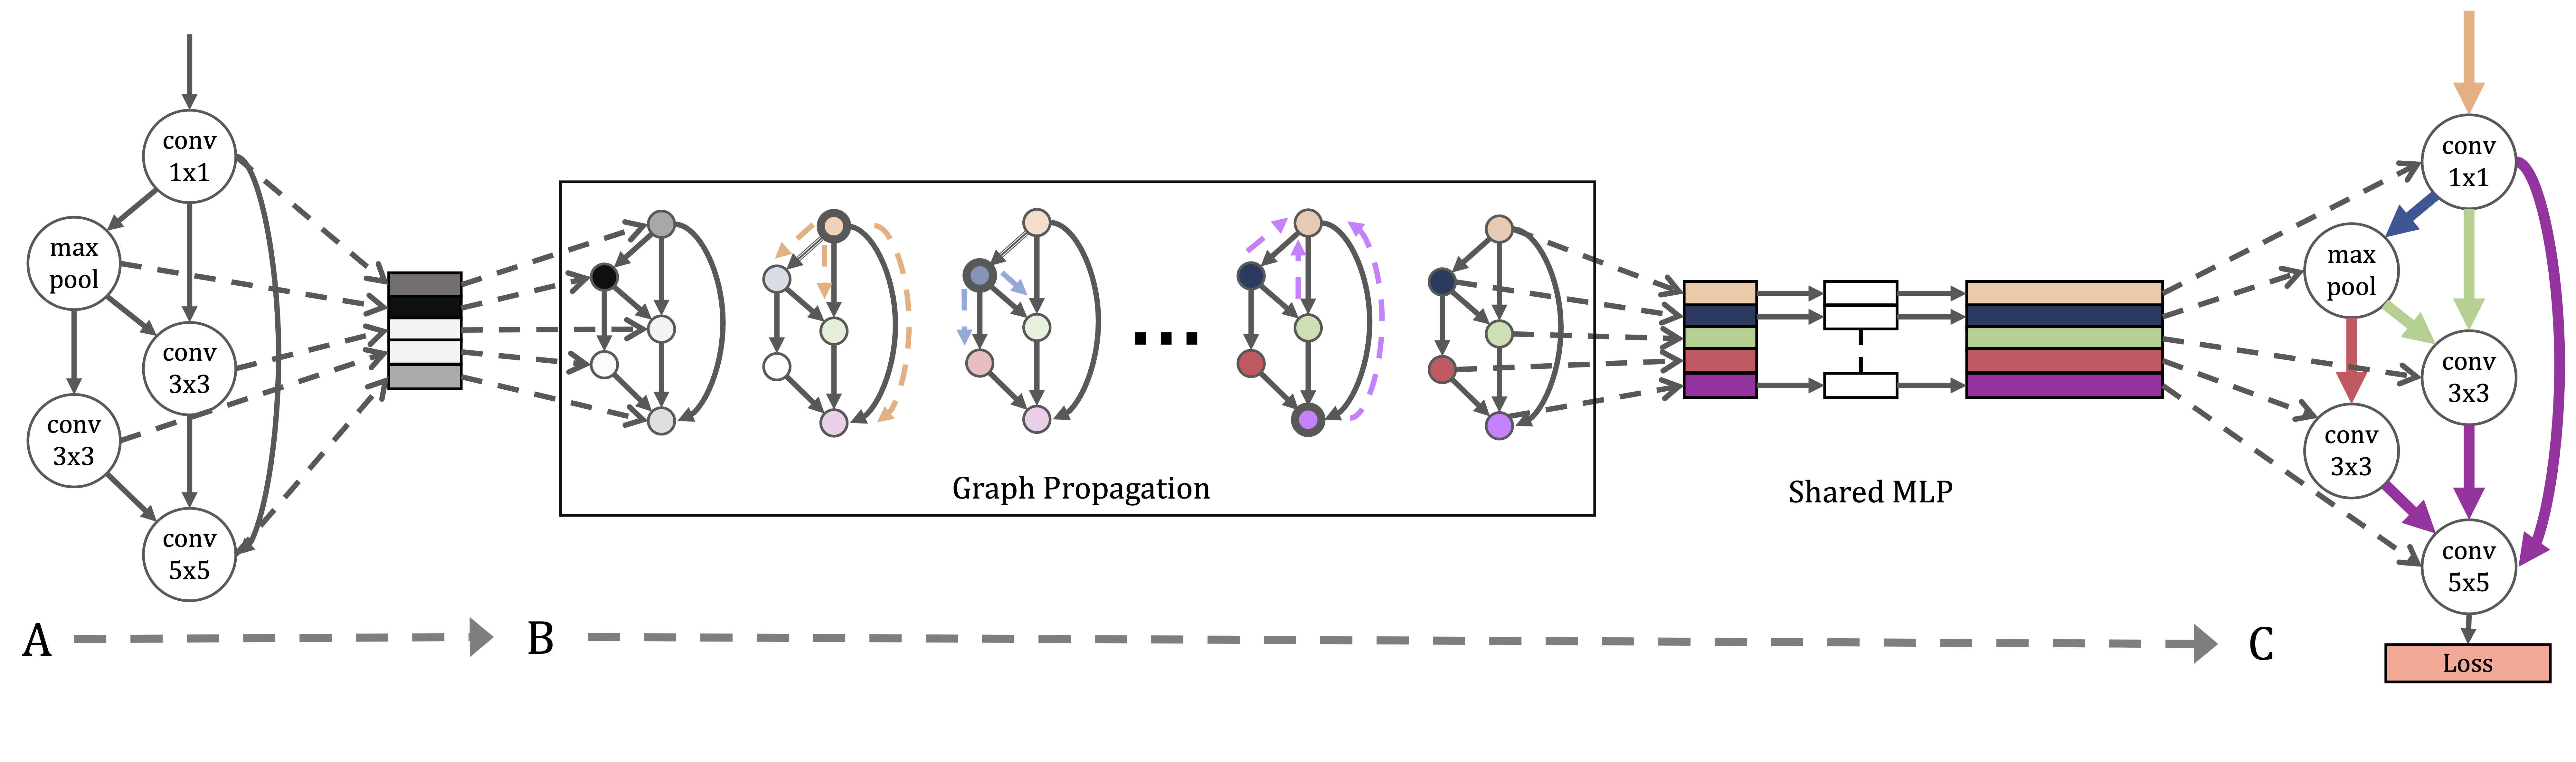
\includegraphics[width=6\linewidth]{figures/main3.png}
\else
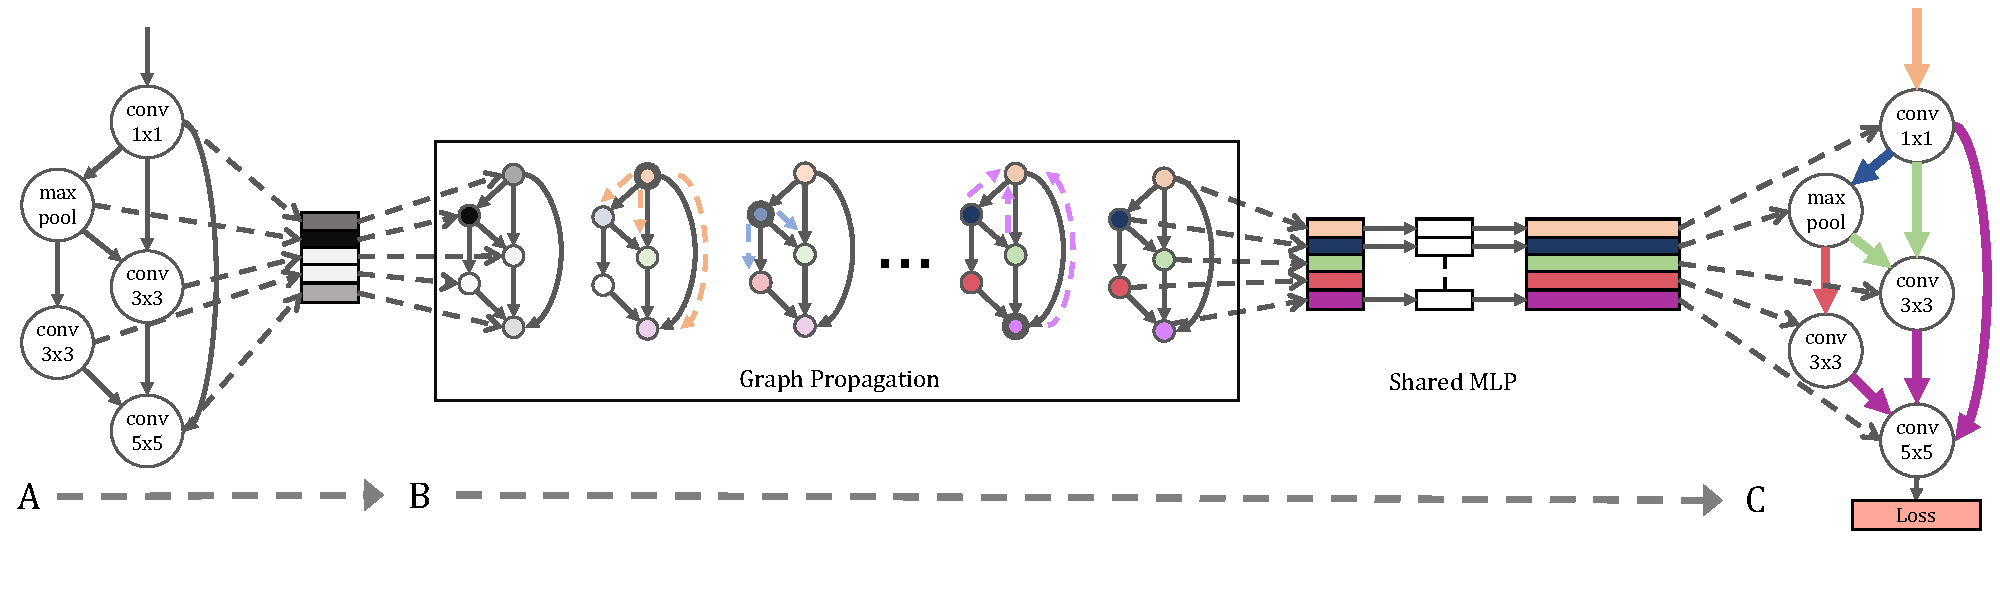
\includegraphics[width=\linewidth]{figures/main3.pdf}
\fi
\vspace{-1cm}
\caption{Our system diagram. \textbf{A}: A neural network architecture
is randomly sampled, forming a GHN. \textbf{B}: After graph propagation, each node in the GHN
generates its own weight parameters. \textbf{C}: The GHN is trained to minimize the training loss of
the sampled network with the generated weights. Random networks are ranked according to their
performance using GHN generated weights. }
\label{fig:main}
\vspace{-0.3cm}
\end{figure}

\subsection{Graphical Representation}
We represent a given architecture as a directed acyclic graph $\gA = (\gV, \gE)$, where each node $v
\in \gV$  has an associated computational operator $f_v$ parametrized by $w_v$, which produces an
output activation tensor $x_v$. Edges $e_{u \mapsto v} = (u, v) \in \gE$ represent the flow of
activation tensors from node $u$ to node $v$. $x_v$ is computed by applying its associated
computational operator on each of its inputs and taking summation as follows
\begin{equation}
\label{eq:compute_node}
x_v = \sum_{e_{u \mapsto v} \in \gE} f_v(x_u; w_v), \ \ \forall v \in \gV.
\end{equation}

\subsection{Graph Hypernetwork}
Our proposed Graph Hypernetwork is defined as a composition of a GNN and a hypernetwork. First,
given an input architecture, we used the graphical representation discussed above to form a graph
$\gA$. A parallel GNN $G_\gA$ is then constructed to be \textit{homomorphic} to $\gA$ with the exact
same topology. Node embeddings are initialized to one-hot vectors representing the node's
computational operator. After graph message-passing steps, a hypernet uses the node embeddings to
generate each node's associated parameters. Let $\vh_v^{(T)}$ be the embedding of node $v$ after $T$
steps of GNN propagation, and let $H \left(\cdot; \vvphi\right)$ be a hypernetwork parametrized by
$\vvphi$, the generated parameters $\tilde{\vw}_v$ are:
\begin{equation}
\tilde{\vw}_v = H \left(\vh_v^{(T)}; \vvphi\right).
\end{equation}
For simplicity, we implement $H$ with a multilayer perceptron (MLP). It is important to note that
$H$ is shared across all nodes, which can be viewed as an output prediction branch in each node of
the GNN. 
Thus the final set of generated weights of the entire architecture $\tilde{\vw}$ is found by applying $H$ on all the nodes and their respective embeddings which are computed by $G_\gA$:
\begin{align}
\tilde{\vw}=\left\{\tilde{\vw}_v | \ v \in \gV  \right\}
   &= \left\{H\left(\vh_v^{(T)}; \vvphi\right) \big| \ v \in \gV  \right\} \\
  &=  \left\{H\left(\vh; \vvphi\right) \big| \ \vh \in G_\gA^{(T)}\left(\left\{\vh_v^{(0)} \big| v \in \gV \right\}; \vphi\right)\right\} \\
  &= GHN\left(\gA; \vphi, \vvphi\right).
\end{align}

\subsection{Architectural Motifs and Stacked GNNs}
\label{section:graph_cells}

\iflatexml
\begin{figure}
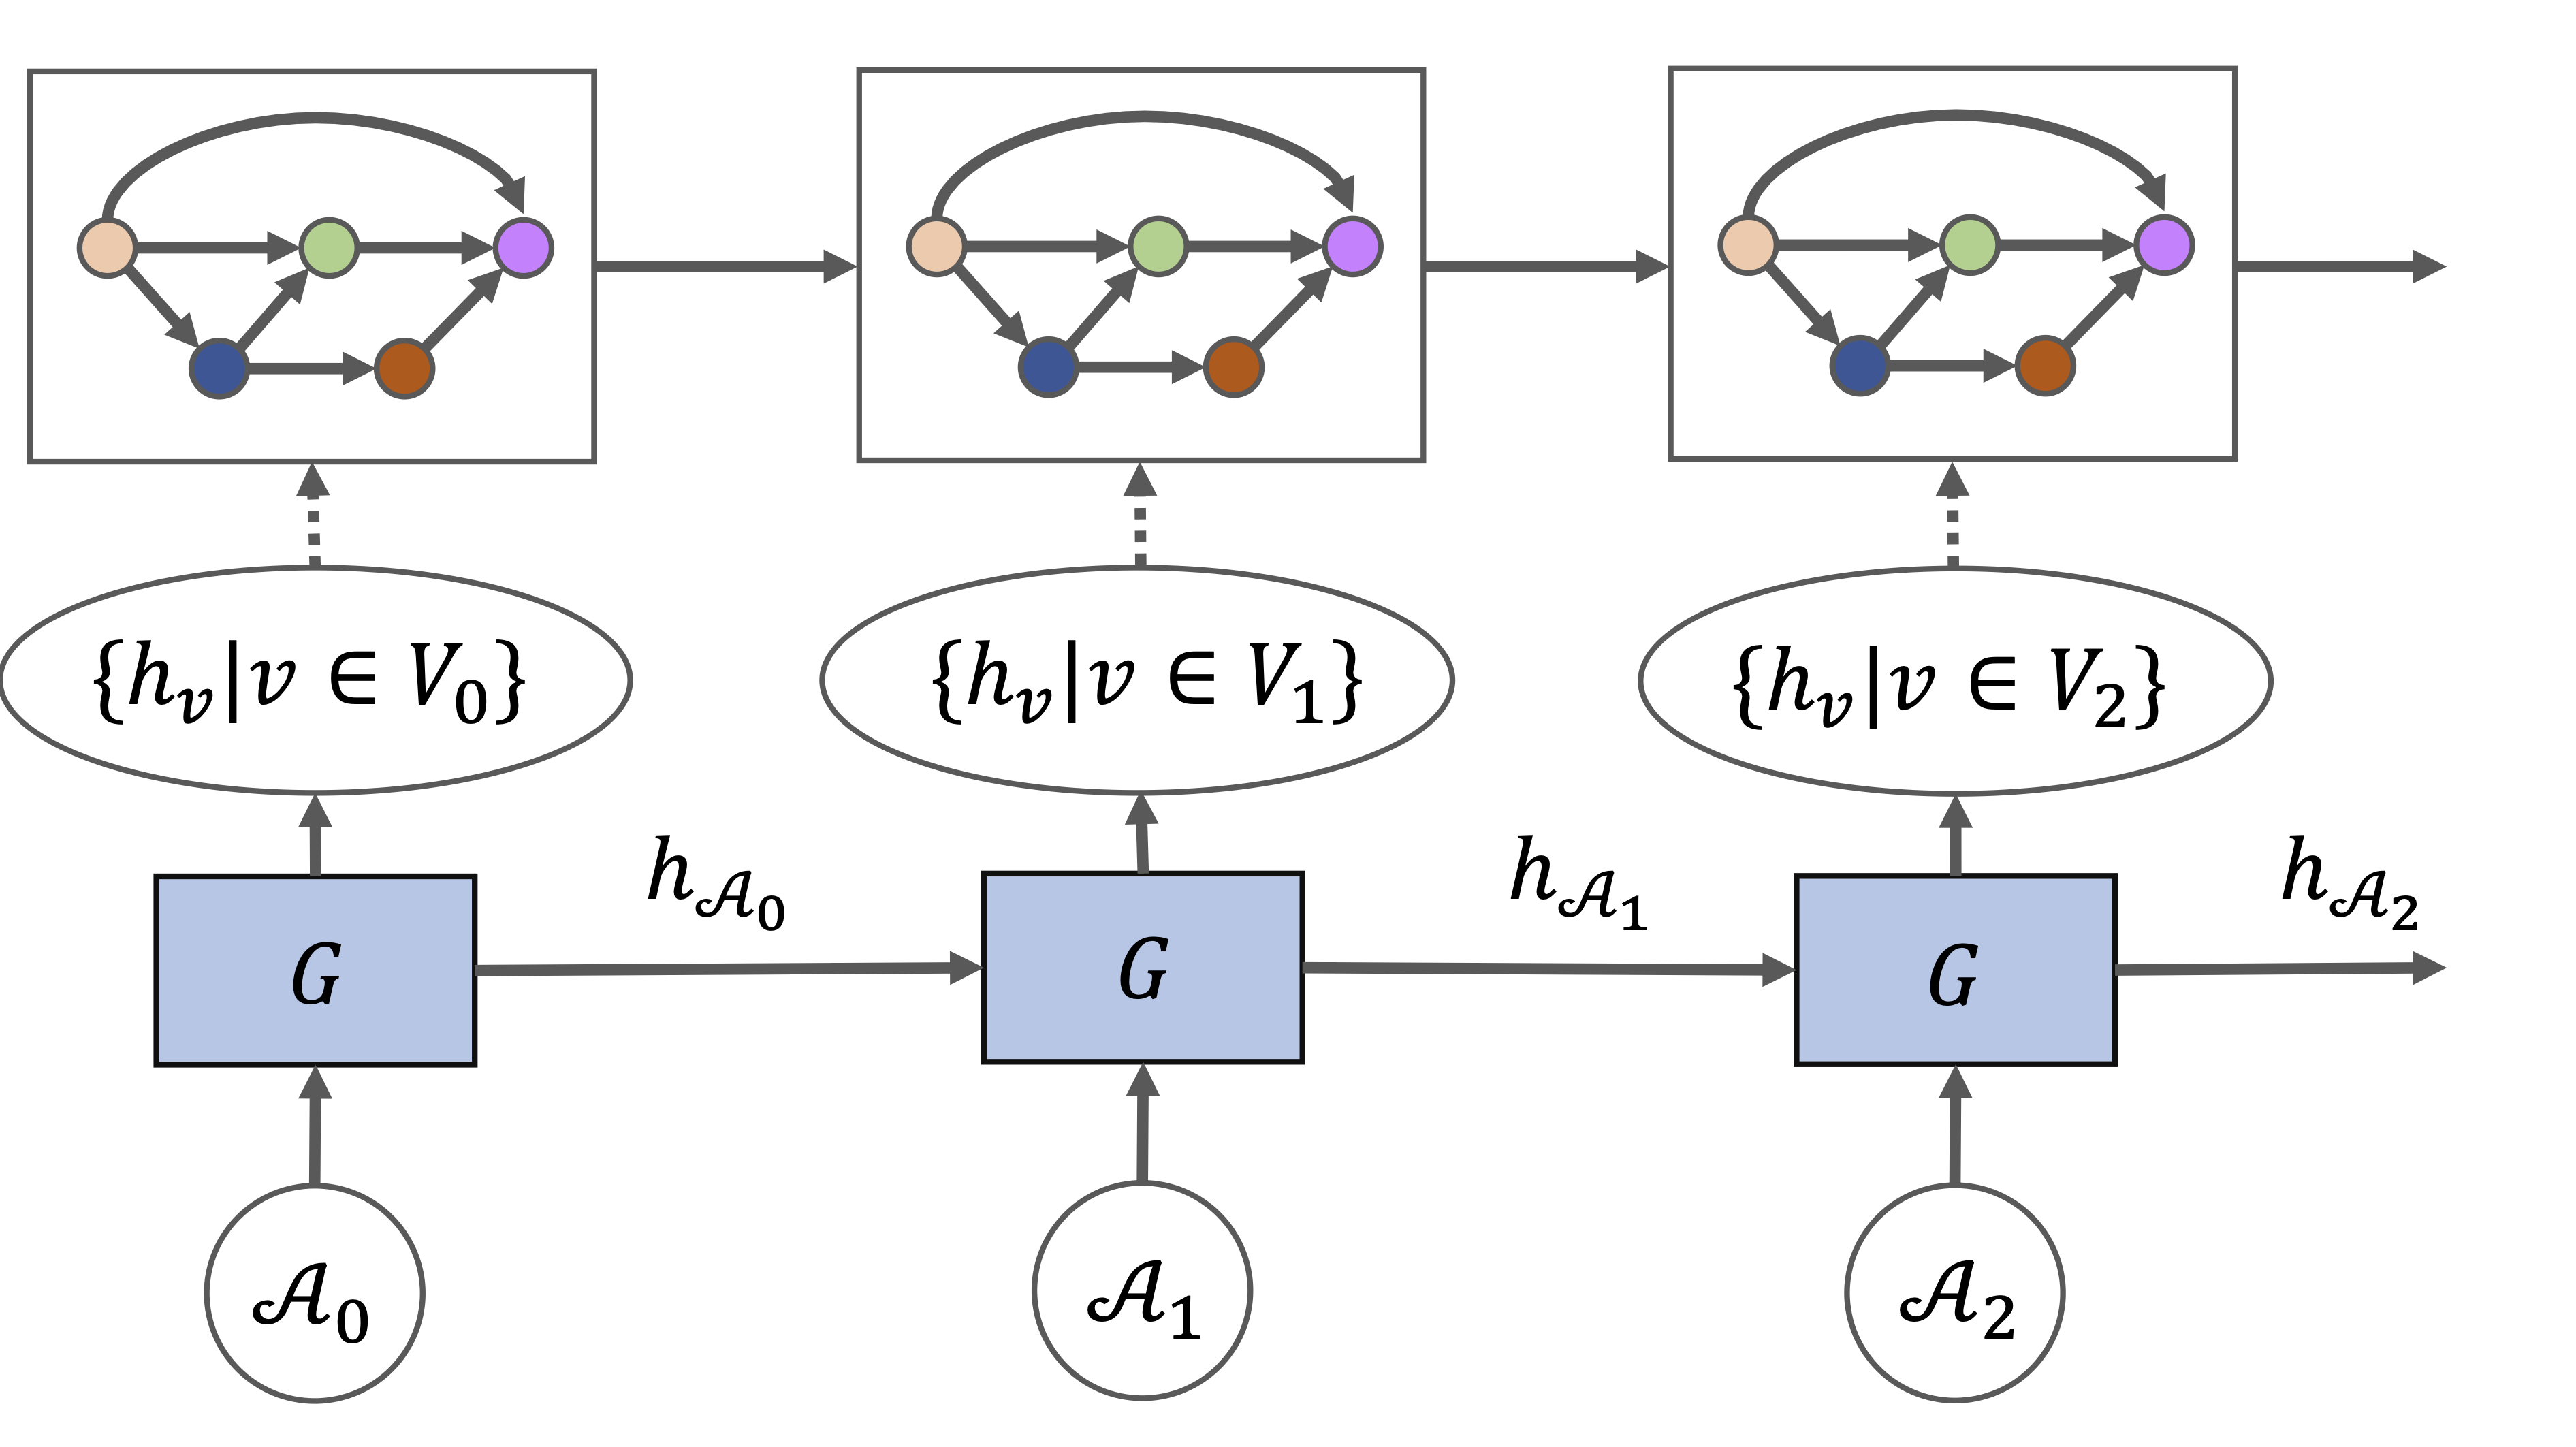
\includegraphics[width=4\linewidth]{figures/graph_cells.png}
\caption{Stacked GHN along the depth dimension.}
\label{fig:graph_cells}
\end{figure}
\else
\begin{wrapfigure}[]{r}{0.33\textwidth}
\vspace*{-0.5cm}
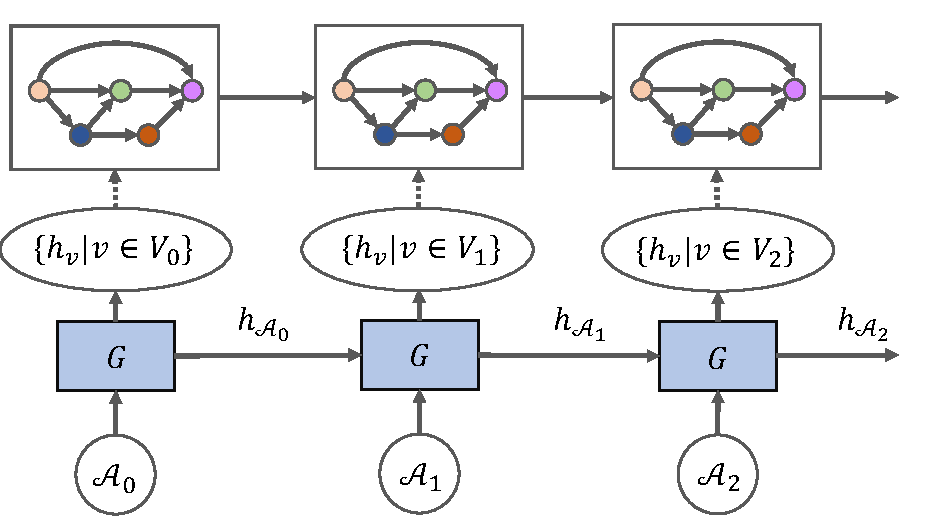
\includegraphics[width=\linewidth]{figures/graph_cells.pdf}
\caption{Stacked GHN along the depth dimension.}
\label{fig:graph_cells}
\end{wrapfigure}
\fi
The computation graph of some popular CNN architectures often spans over hundreds of nodes
\citep{he2016deep,huang2017densely}, which makes the search problem scale poorly. Repeated
architecture motifs are originally exploited in those architectures where the computation of each
computation block at different resolutions is the same, e.g. ResNet \citep{he2016resnet}. Recently,
the use of architectural motifs also became popular in the context of neural architecture search,
e.g. \citep{zoph2017learning, pham2018efficient}, where a small graph module with a fewer number of
computation nodes is searched, and the final architecture is formed by repeatedly stacking the same
module. \cite{zoph2017learning} showed that this leads to stronger performance due to a reduced
search space; the module can also be transferred to larger datasets by adopting a different
repeating pattern.

Our proposed method scales naturally with the design of repeated modules by stacking the same graph
hypernetwork along the depth dimension. Let $\gA$ be a graph composed of a chain of repeated modules
$\{\gA_i\}_{i=1}^N$. A graph level embedding $\vh_{\gA_i}$ is computed by taking an average over all
node embeddings after a full propagation of the current module, and passed onwards to the input node
of the next module as a message before graph propagation continues to the next module.
\begin{align}
\vh_{\gA_0} &= 0,\\
\vh_{\gA_i} &= \frac{1}{|\gV_i|}\sum_{v\in \gV_i} \left\{\vh_v^{(T)} | v \in \gV_i \right\} \label{eq:agg}\\
            &= \frac{1}{|\gV_i|}\sum G_{\gA_i}^{(T)}\left(\left\{\vh_v^{(0)} | v \in \gV_i \right\}, \vh_{\gA_{i-1}}; \vphi\right) \ \ \forall i > 0 \label{eq:next_cell}
\end{align}
Note that $G_{\gA_i}$ share parameters for all $\gA_i$.  Please see Figure~\ref{fig:graph_cells} for an overview.

\subsection{Forward-backward GNN message passing}
\label{sec:prop_scheme}
Standard GNNs employ the \textit{synchronous propagation scheme} \citep{li2015gated}, where the node
embeddings of all nodes are updated simultaneously at every step (see Equation~\ref{eq:gnn_prop}).
Recently, \cite{liao2018graph} found that such propagation scheme is inefficient in passing
long-range messages and suffers from the vanishing gradient problem as do regular RNNs. To mitigate
these shortcomings they proposed \textit{asynchronous propagation} using graph partitions. In our
application domain, deep neural architectures are chain-like graphs with a long diameter; This can
make synchronous message passing difficult. Inspired by the backpropagation algorithm, we propose
another variant of asynchronous propagation scheme, which we called \textit{forward-backward}
propagation, that directly mimics the order of node execution in a backpropagation algorithm.
Specifically, let $s$ be a topological sort of the nodes in the computation graph in a forward pass,
\begin{equation}
\label{eq:gnn_prop2}
\vh_v^{(t+1)} = 
\begin{cases}
U \left(\vh_v^{(t)}, \vm_v^{(t)} \right) \ \ & \text{if } s(t) = v \text{ and } 1 \le t \le |\gV|\\
  \ \ & \text{or if } s(2|\gV| - t) = v \text{ and } |\gV| + 1 \le t < 2|\gV|,\\
\vh_v^{(t)} \ \ & \text{otherwise}.
\end{cases}
\end{equation}
The total number of propagation steps $T$ for a full forward-backward pass will then become $2|\gV|-1$. Under the synchronous scheme,  propagating information across a graph with diameter $|\gV|$ would require $O(|\gV|^2)$ messages. This is reduced to $O(|\gV|)$ under the forward-backward scheme.

\subsection{Learning}
Learning a graph hypernetwork is straightforward since $\tilde{\vw}$ are directly generated by a
differentiable network. We compute gradients of the graph hypernetwork parameters $\vphi, \vvphi$
using the chain rule:
\begin{equation}
\nabla_{\vphi, \vvphi}{\gL_{train}(\tilde{\vw})} = \nabla_{\tilde{\vw}}{
\gL_{train}(\tilde{\vw})} \cdot \nabla_{\vphi, \vvphi}{\tilde{\vw}}
\end{equation}
The first term is the gradients of standard network parameters, the second term is decomposed as\begin{align}
 \nabla_\vphi{\tilde{\vw}} &= \left\{ \nabla_\vh H( \vh; \vvphi) \cdot \nabla_\vphi \vh \ \big| \ \vh \in G^{(T)} \left( \{\vh_v^{(0)}\}, \gA, \vphi \right) \right\}, \label{eq:gnn_grad}  \\ 
 \nabla_\vvphi{\tilde{\vw}} &= \left\{ \nabla_\vvphi H( \vh_v^{(T)}; \vvphi) \ \big| \ v \in \gV \right\} \label{eq:hypernet_grad}
\end{align}
where (Eq. \ref{eq:gnn_grad}) is the contribution from GNN module $G$ and (Eq.
\ref{eq:hypernet_grad}) is the contribution from the hypernet module $H$. Both $G$ and $H$ are
jointly learned throughout training.
% !TEX root = ../main.tex

\section{Experiments}

To test the effectiveness of our reweighting algorithm, we designed both class imbalance and noisy
label settings, and a combination of both, on standard MNIST and CIFAR benchmarks for image
classification using deep CNNs.
\footnote{Code released at: \url{https://github.com/uber-research/learning-to-reweight-examples}}
% !TEX root = ../main.tex

\subsection{MNIST data imbalance experiments} 

We use the standard MNIST handwritten digit classification dataset and subsample the dataset to
generate a class imbalance binary classification  task. We select a total of 5,000 images of size
28$\times$28 on class 4 and 9, where 9 dominates the training data distribution. We train a standard
LeNet on this task and we compare our method with a suite of commonly used tricks for class
imbalance: 1) \textsc{Proportion} weights each example by the inverse frequency 2) \textsc{Resample}
samples a class-balanced mini-batch for each iteration 3) \textsc{Hard Mining} selects the highest
loss examples from the majority class and 4) \textsc{Random} is a random example weight baseline
that assigns weights based on a rectified Gaussian distribution:
\begin{equation}
w_i^{\text{rnd}} = \frac{\max(z_i, 0)}{\sum_i \max(z_i, 0)},
\label{eq:randomwts}
\end{equation}
where $z_i \sim \mathcal{N}(0, 1)$.
To make sure that our method does
not have the privilege of training on more data, we split the balanced validation set of 10 images
directly from the training set. The network is trained with SGD with a learning rate of 1e-3 and
mini-batch size of 100 for a total of 8,000 steps.

Figure~\ref{fig:mnist_imba} plots the test error rate across various imbalance ratios averaged from
10 runs with random splits. Note that our method significantly outperforms all the baselines. With
class imbalance ratio of 200:1, our method only reports a small increase of error rate around 2\%,
whereas other methods suffer terribly under this setting. Compared with resampling and hard negative
mining baselines, our approach does not throw away samples based on its class or training loss - as
long as a sample is helpful towards the validation loss, it will be included as a part of the
training loss.

% !TEX root = ../main.tex

\begin{figure}
\centering
\iflatexml
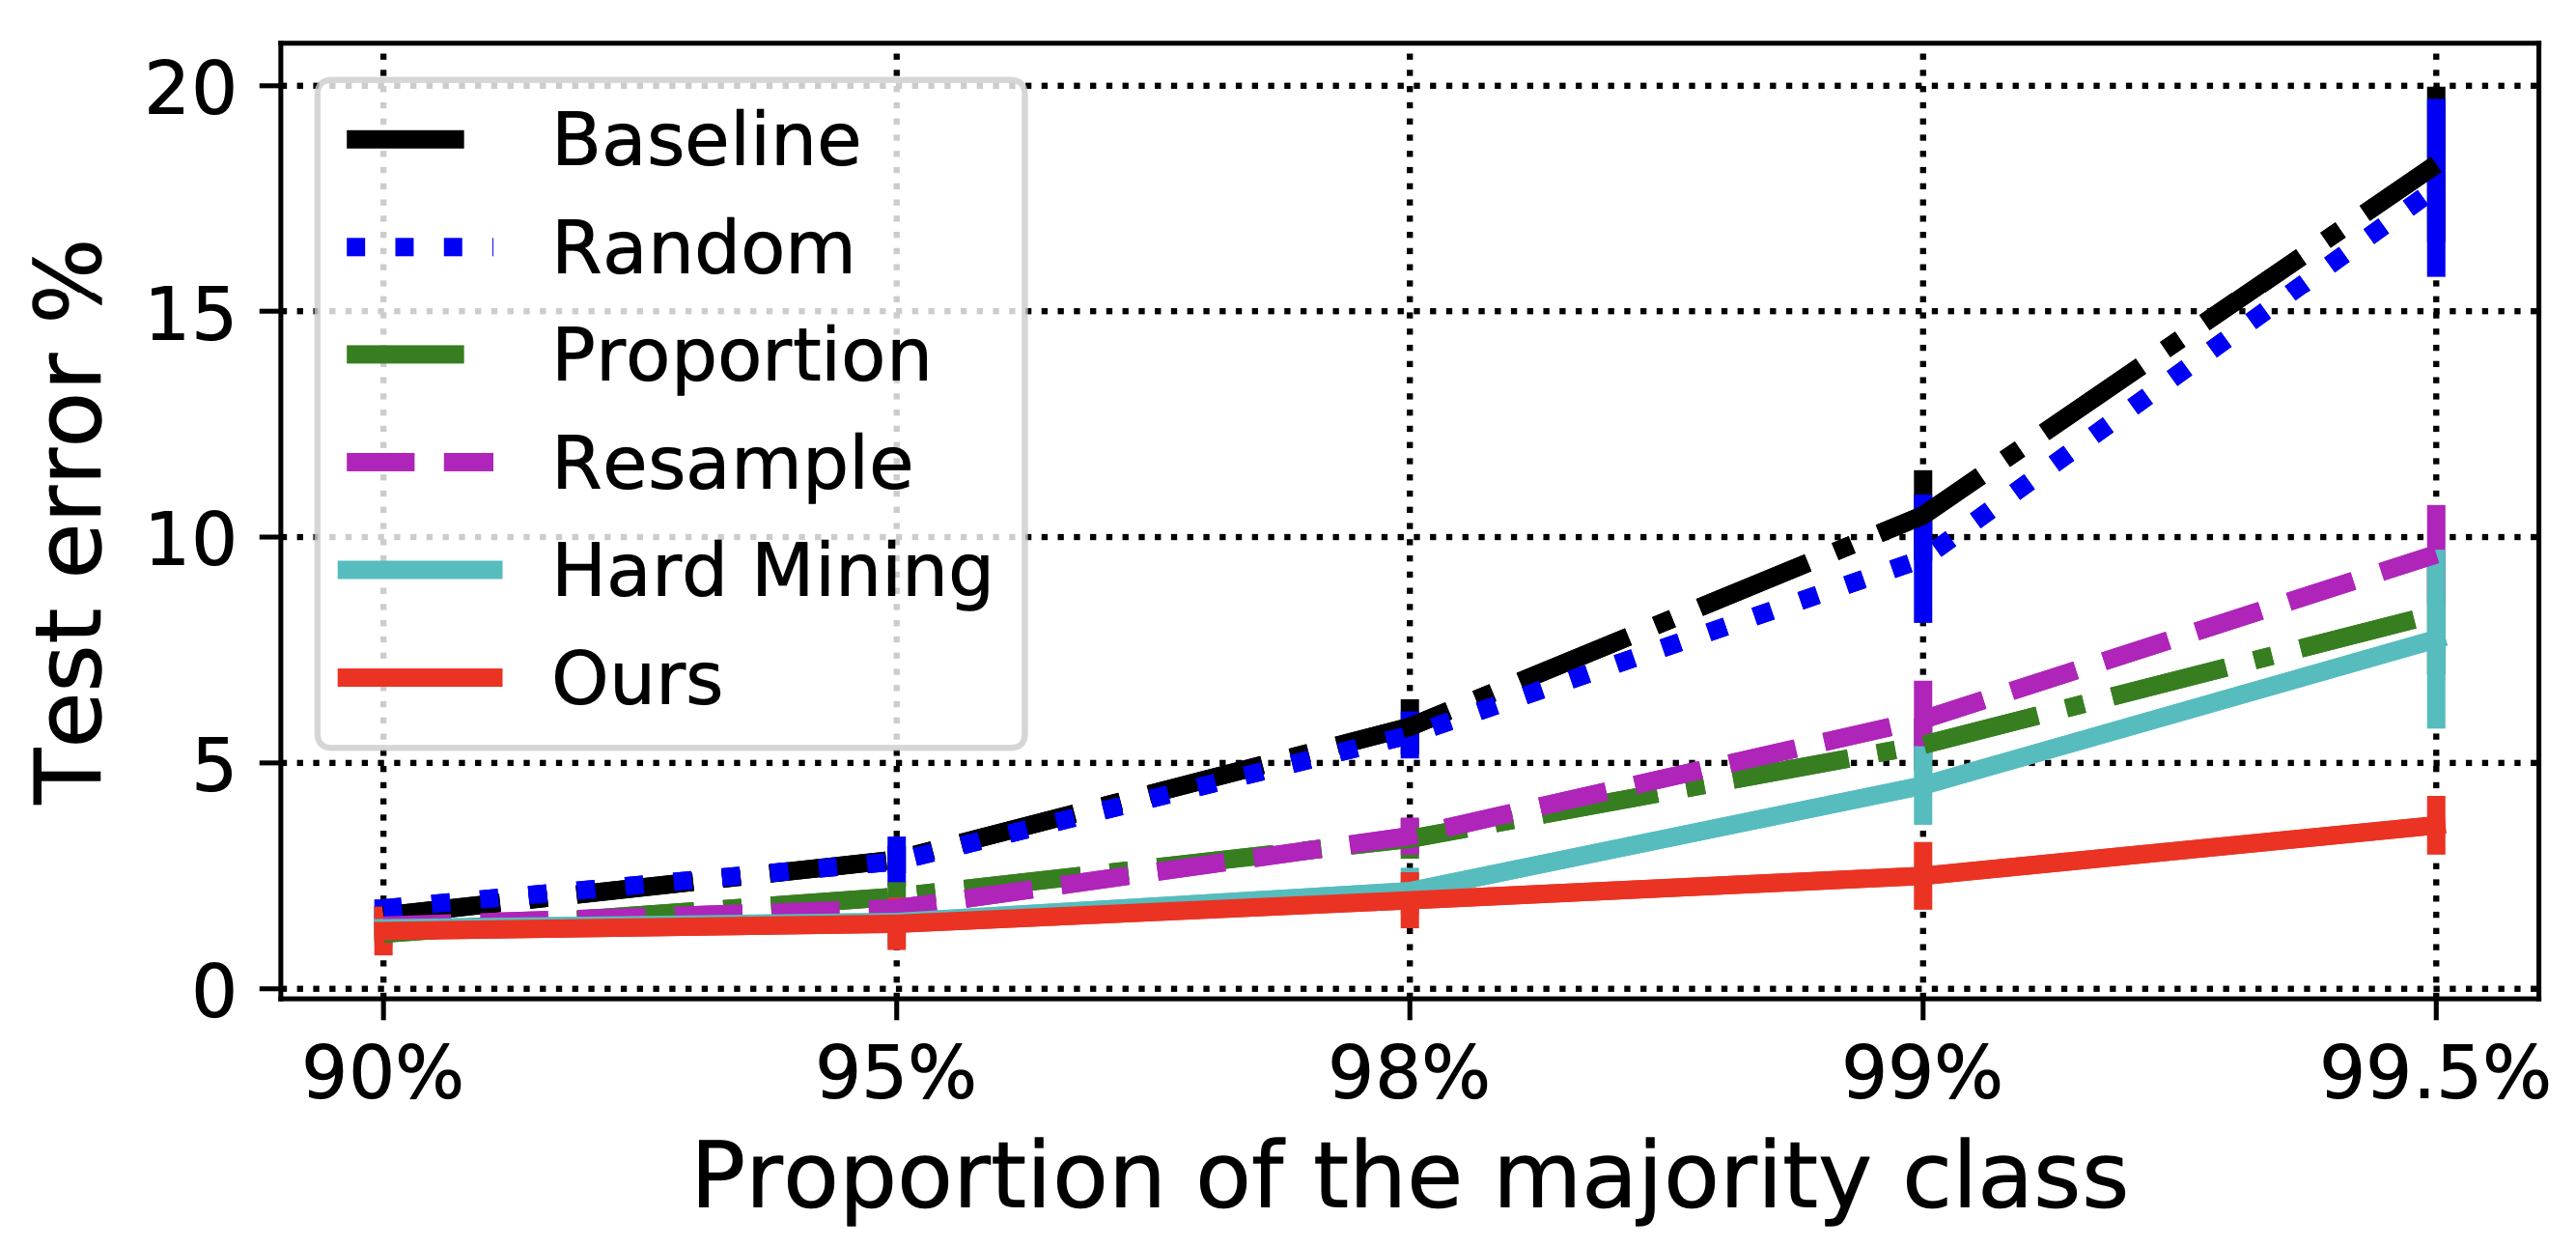
\includegraphics[width=6\columnwidth]{figures/mnist-imbalance.png}
\else
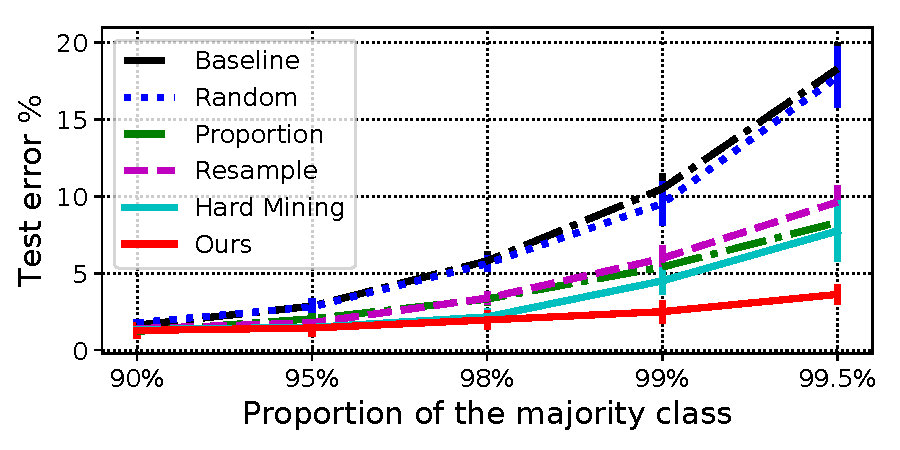
\includegraphics[width=0.9\columnwidth]{figures/mnist-imbalance.pdf}
\fi
\vspace{-0.1in}
\caption{MNIST 4-9 binary classification error using a LeNet on imbalanced classes. Our method uses a small balanced validation split of 10 examples.}
\label{fig:mnist_imba}
\end{figure}


% !TEX root = ../main.tex
\subsection{CIFAR noisy label experiments}

Reweighting algorithm can also be useful on datasets where the labels are noisy. We study two
settings of label noise here: 
\begin{itemize}
    \vspace{-0.1in}

    \item \textsc{UniformFlip}: All label classes can uniformly flip to any other label classes,
which is the most studied in the literature.

    \vspace{-0.1in}

    \item \textsc{BackgroundFlip}: All label classes can flip to a single background class. This
noise setting is very realistic. For instance, human annotators may not have recognized all the
positive instances, while the rest remain in the background class. This is also a combination of
label imbalance and label noise since the background class usually dominates the label distribution.

\end{itemize}
We compare our method with prior work on the noisy label problem.
\vspace{-0.1in}
\begin{itemize}
\item \textsc{Reed}, proposed by \citet{reed14noisy}, is a bootstrapping technique where the
training target is a convex combination of the model prediction and the label.

\item \textsc{S-Model}, proposed by \citet{goldberger17noise}, adds a fully connected softmax layer
after the regular classification output layer to model the noise transition matrix.

\item \textsc{MentorNet}, proposed by \citet{jiang17mentornet}, is an RNN-based meta-learning model
that takes in a sequence of loss values and outputs the example weights. We compare numbers reported
in their paper with a base model that achieves similar test accuracy under 0\% noise.
\end{itemize}
In addition, we propose two simple baselines: 
1) \textsc{Random}, which assigns weights according to a rectified Gaussian (see
   Eq.~\ref{eq:randomwts});
2) \textsc{Weighted}, designed for \textsc{BackgroundFlip}, where the model
knows the oracle noise ratio for each class and reweights the training loss proportional to the
percentage of clean images of that label class.
\vspace{-0.05in}
\paragraph{Clean validation set} For \textsc{UniformFlip}, we use 1,000 clean images in the
validation set; for \textsc{BackgroundFlip}, we use 10 clean images per label class. Since our
method uses information from the clean validation, for a fair comparison, we conduct an additional
finetuning on the clean data based on the pre-trained baselines. We also study the effect on the
size of the clean validation set in an ablation study.
\vspace{-0.05in}
\paragraph{Hyper-validation set} For monitoring training progress and tuning baseline
hyperparameters, we split out another 5,000 hyper-validation set from the 50,000 training images. We
also corrupt the hyper-validation set with the same noise type.
% !TEX root = ../main.tex

\begin{table}[t]
\begin{center}
\caption{CIFAR \textsc{UniformFlip} under 40\% noise ratio using a WideResNet-28-10 model. Test
accuracy shown in percentage. Top rows use only noisy data, and bottom uses additional 1000 clean
images. ``FT'' denotes fine-tuning on clean data.}
\label{tab:uniformflip}
\vskip 0.1in
\begin{small}
\begin{sc}
\begin{tabular}{ccc}
\toprule
Model              &  CIFAR-10                    & CIFAR-100                     \\
\midrule
Baseline           & 67.97 $\pm$ 0.62             & 50.66 $\pm$ 0.24              \\
Reed-Hard          & 69.66 $\pm$ 1.21             & 51.34 $\pm$  0.17             \\
S-Model            & 70.64 $\pm$ 3.09             & 49.10 $\pm$ 0.58              \\
MentorNet          & 76.6                         & 56.9                          \\
Random             & 86.06 $\pm$ 0.32.            & 58.01 $\pm$ 0.37              \\
\midrule
\multicolumn{3}{c}{Using 1,000 clean images} \\
\midrule
Clean Only         & 46.64 $\pm$ 3.90             & 9.94 $\pm$ 0.82               \\
Baseline +FT       & 78.66 $\pm$ 0.44             & 54.52 $\pm$ 0.40              \\
MentorNet +FT      & 78                           & 59                            \\
Random +FT         & 86.55 $\pm$ 0.24             & 58.54 $\pm$ 0.52              \\
Ours               & \textbf{86.92 $\pm$ 0.19}    & \textbf{61.34 $\pm$ 2.06}     \\
\bottomrule
\end{tabular}
\end{sc}
\end{small}
\end{center}
\vskip -0.1in
\end{table}
% !TEX root = ../main.tex

\begin{table}[t]
\begin{center}

\caption{CIFAR \textsc{BackgroundFlip} under 40\% noise ratio using a ResNet-32 model. Test accuracy
shown in percentage. Top rows use only noisy data, and bottom rows use additional 10 clean images
per class. ``+ES'' denotes early stopping; ``FT'' denotes fine-tuning.}

\label{tab:backgroundflip}

\resizebox{\columnwidth}{!}{
\begin{small}
\begin{sc}
\begin{tabular}{ccc}
\toprule
Model                             & CIFAR-10                    & CIFAR-100                     \\
\midrule
Baseline                          & 59.54 $\pm$ 2.16            & 37.82 $\pm$ 0.69              \\
Baseline +ES                      & 64.96 $\pm$ 1.19            & 39.08 $\pm$ 0.65              \\
Random                            & 69.51 $\pm$ 1.36            & 36.56 $\pm$ 0.44              \\
Weighted                          & 79.17 $\pm$ 1.36            & 36.56 $\pm$ 0.44              \\
Reed Soft +ES                     & 63.47 $\pm$ 1.05            & 38.44 $\pm$ 0.90              \\
Reed Hard +ES                     & 65.22 $\pm$ 1.06            & 39.03 $\pm$ 0.55              \\
S-Model                           & 58.60 $\pm$ 2.33            & 37.02 $\pm$ 0.34              \\
S-Model +Conf                     & 68.93 $\pm$ 1.09            & 46.72 $\pm$ 1.87              \\
S-Model +Conf +ES                 & 79.24 $\pm$ 0.56            & 54.50 $\pm$ 2.51              \\
\midrule
\multicolumn{3}{c}{Using 10 clean images per class} \\
\midrule
Clean Only                        & 15.90 $\pm$ 3.32            & 8.06  $\pm$ 0.76              \\
Baseline +FT                      & 82.82 $\pm$ 0.93            & 54.23 $\pm$ 1.75              \\
Baseline +ES +FT                  & 85.19 $\pm$ 0.46            & 55.22 $\pm$ 1.40              \\
Weighted +FT                      & 85.98 $\pm$ 0.47            & 53.99 $\pm$ 1.62              \\
S-Model +Conf +FT                 & 81.90 $\pm$ 0.85            & 53.11 $\pm$ 1.33              \\
S-Model +Conf +ES +FT             & 85.86 $\pm$ 0.63            & 55.75 $\pm$ 1.26              \\
Ours                              & \textbf{86.73 $\pm$ 0.48}   & \textbf{59.30 $\pm$ 0.60}     \\
\bottomrule
\end{tabular}
\end{sc}
\end{small}
}
\end{center}
\vskip -0.1in
\end{table}
\vspace{-0.05in}
\paragraph{Experimental details} For \textsc{Reed} model, we use the best $\beta$ reported in
\citet{reed14noisy} ($\beta=0.8$ for hard bootstrapping and $\beta=0.95$ for soft bootstrapping).
For the \textsc{S-Model}, we explore two versions to initialize the transition weights: 1) a
smoothed identity matrix; 2) in background flip experiments we consider initializing the transition
matrix with the confusion matrix of a pre-trained baseline model (\textsc{S-Model +Conf}). We find
baselines can easily overfit the training noise, and therefore we also study early stopped versions
of the baselines to provide a stronger comparison. In contrast, we find early stopping not necessary
for our method.

To make our results comparable with the ones reported in \textsc{MentorNet} and to save computation
time, we exchange their Wide ResNet-101-10 with a Wide ResNet-28-10 (WRN-28-10) \cite{wrn} with
dropout 0.3 as our base model in the \textsc{UniformFlip} experiments. We find that test accuracy
differences between the two base models are within 0.5\% on CIFAR datasets under 0\% noise. In the
\textsc{BackgroundFlip} experiments, we use a ResNet-32 \cite{resnet} as our base model.

We train the models with SGD with momentum, at an initial learning rate 0.1 and a momentum 0.9 with
mini-batch size 100. For ResNet-32 models, the learning rate decays $\times 0.1$ at 40K and 60K
steps, for a total of 80K steps. For WRN and early stopped versions of ResNet-32 models, the
learning rate decays at 40K and 50K steps, for a total of 60K steps. Under regular 0\% noise
settings, our base ResNet-32 gets 92.5\% and 68.1\% classification accuracy on CIFAR-10 and 100, and
the WRN-28-10 gets 95.5\% and 78.2\%. For the finetuning stage, we run extra 5K steps of training on
the limited clean data.

We report the average test accuracy for 5 different random splits of clean and noisy labels, with
95\% confidence interval in Table~\ref{tab:uniformflip} and \ref{tab:backgroundflip}. The background
classes for the 5 trials are [0, 1, 3, 5, 7] (CIFAR-10) and [7, 12, 41, 62, 85] (CIFAR-100).

% !TEX root = ../main.tex
\begin{figure}[t]
\centering
\iflatexml
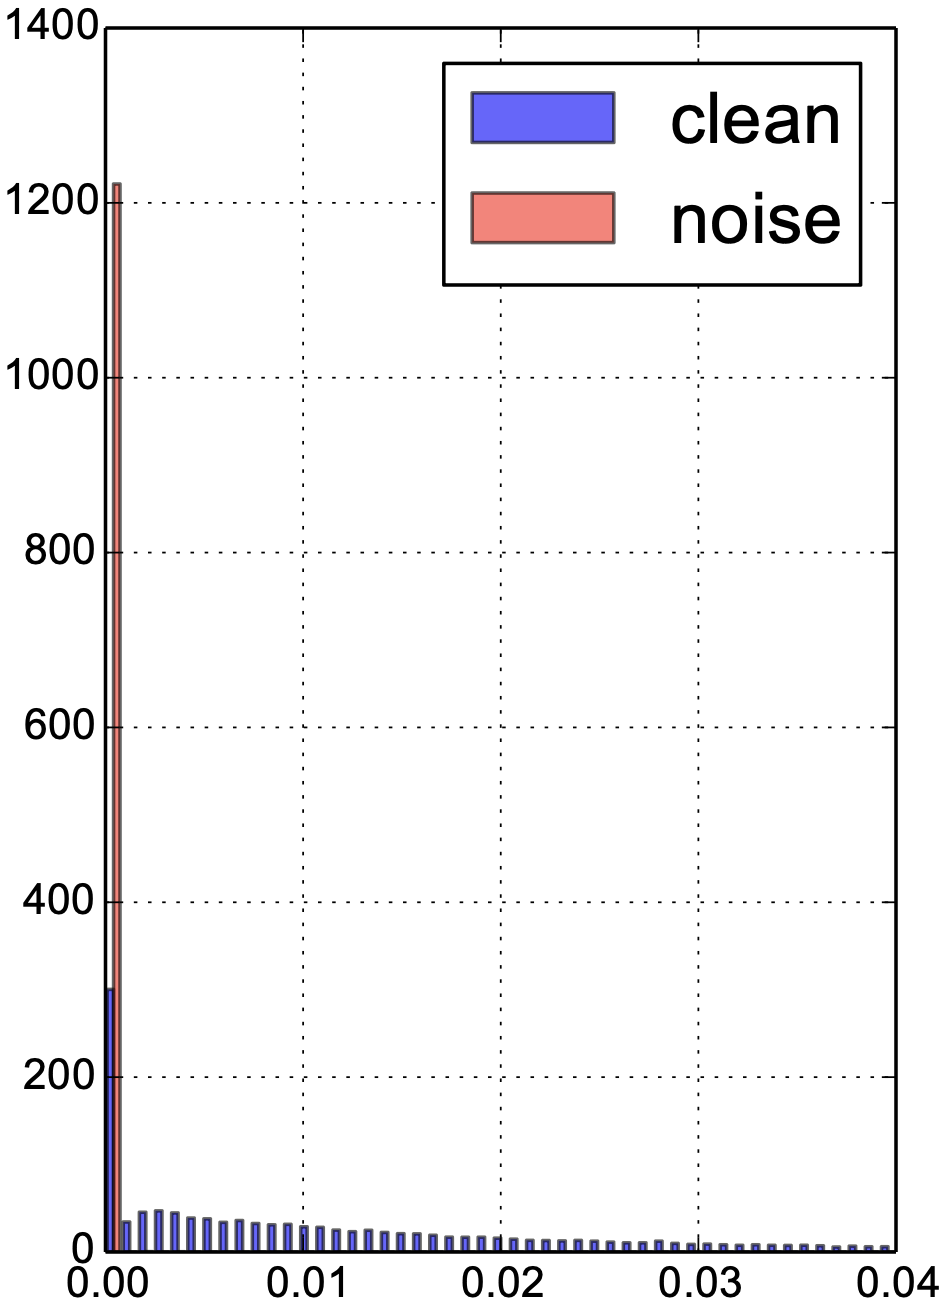
\includegraphics[width=3\columnwidth]{figures/uncondition.png}
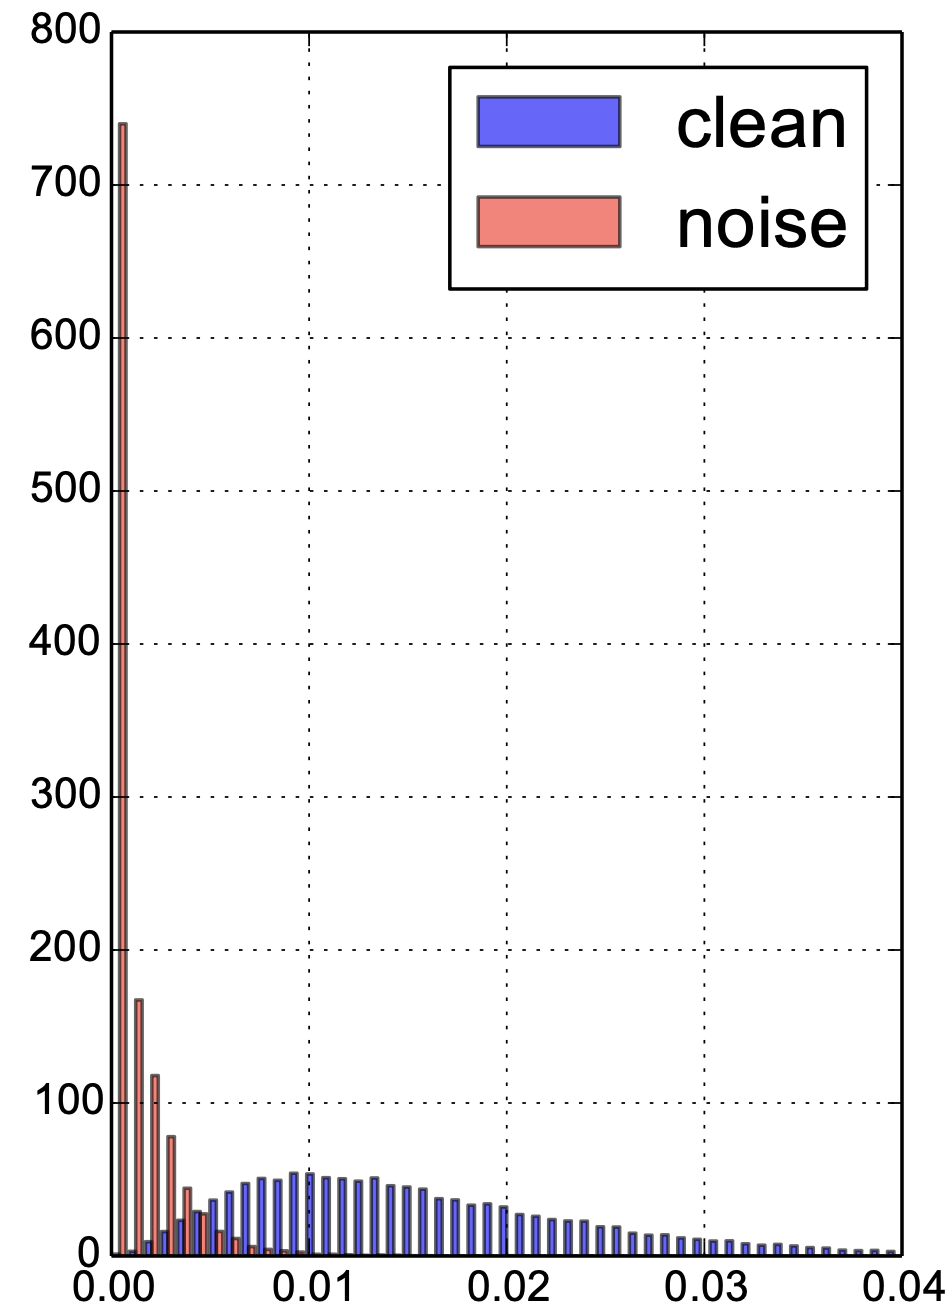
\includegraphics[width=3\columnwidth]{figures/condition.png}
\else
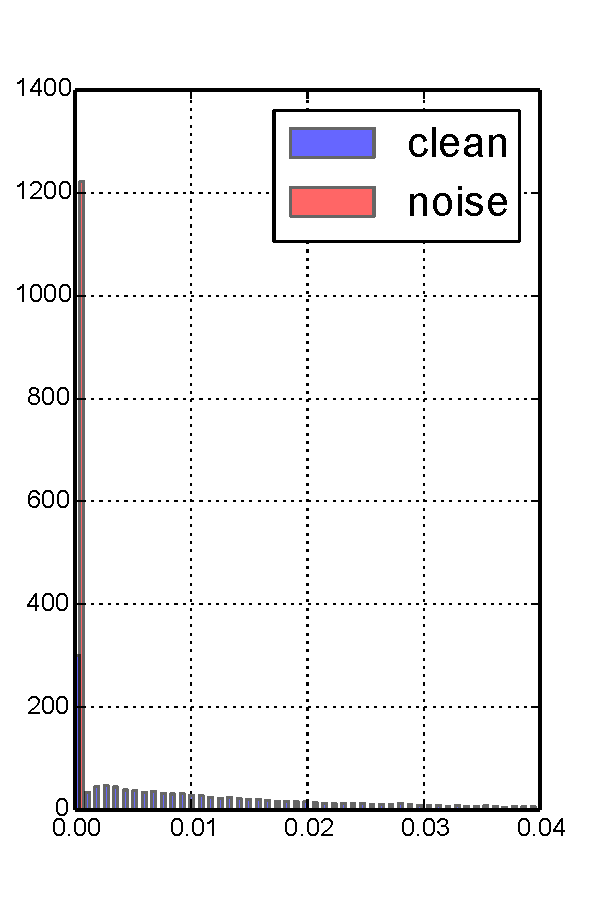
\includegraphics[width=0.45\columnwidth,trim={0cm 0 0cm 0},clip]{figures/uncondition.pdf}
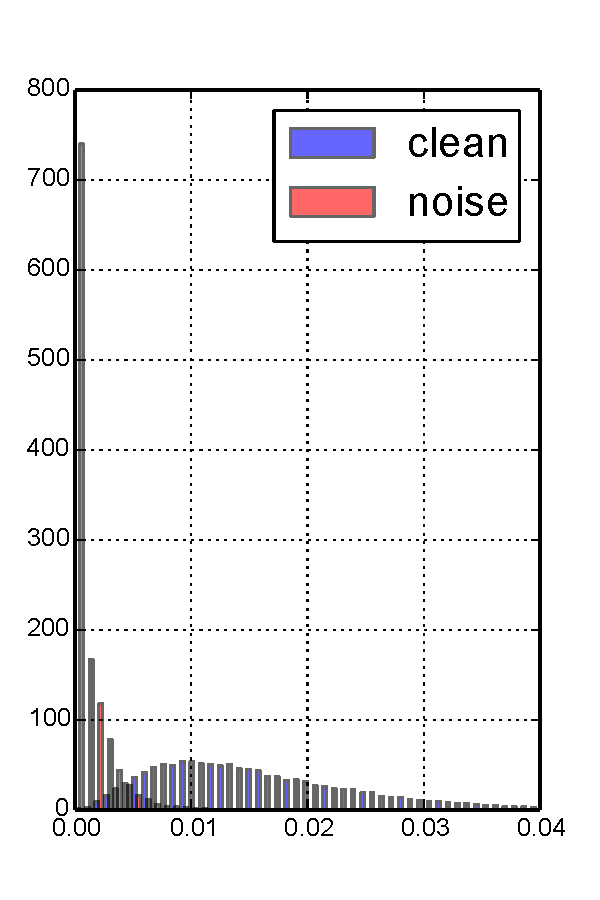
\includegraphics[width=0.45\columnwidth,trim={0cm 0 0cm 0},clip]{figures/condition.pdf}
\fi
\vspace{-0.1in}
\caption{Example weights distribution on \textsc{BackgroundFlip}. Left: a hyper-validation batch,
with randomly flipped background noises. Right: a hyper-validation batch containing only on a single
label class, with flipped background noises, averaged across all non-background classes.}
\label{fig:dist}
\end{figure}

% !TEX root = ../main.tex

\begin{figure}[t]
\centering
\iflatexml
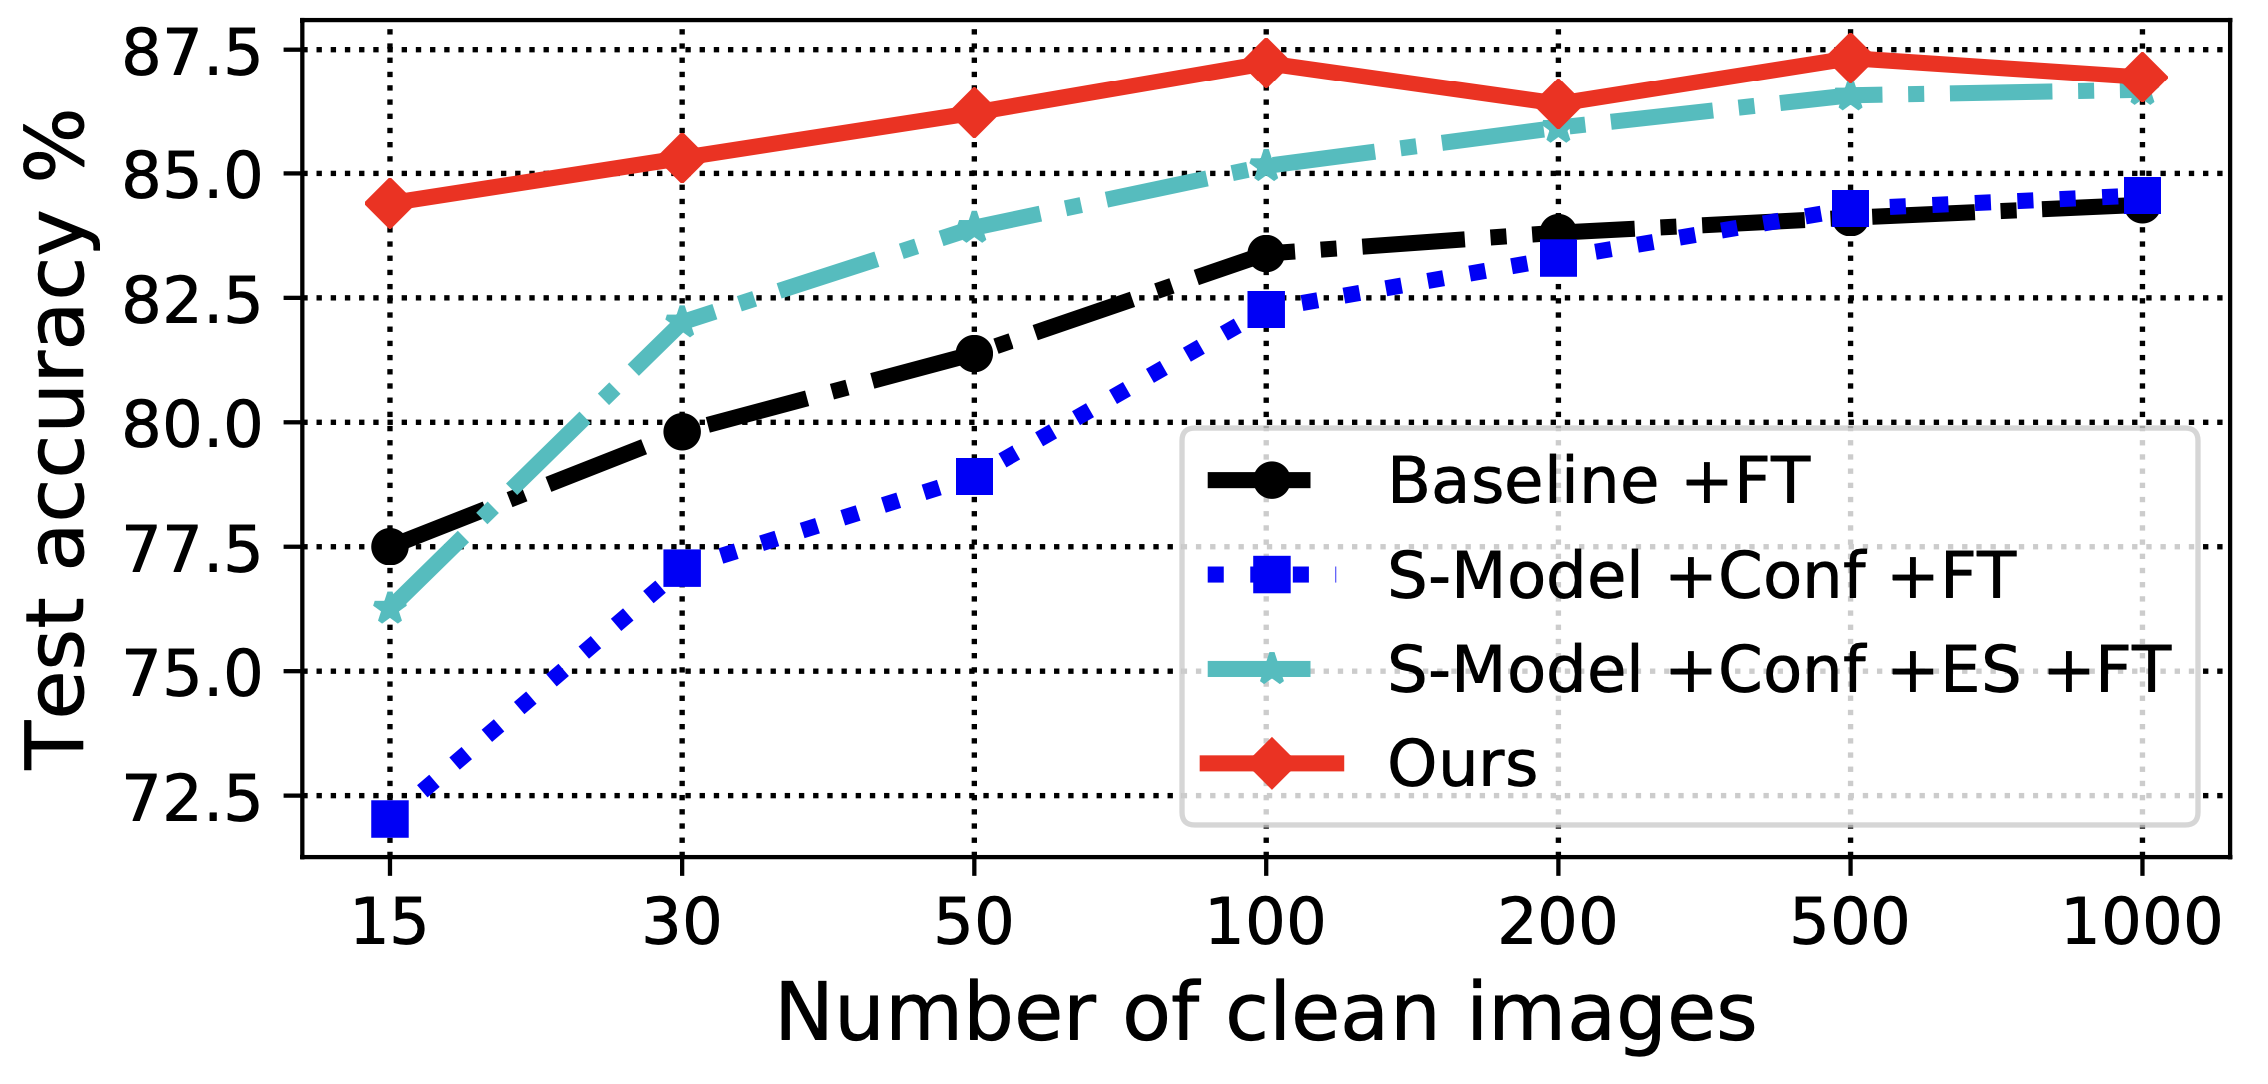
\includegraphics[width=6\columnwidth]{figures/cifar-imbalance-ft.png}
\else
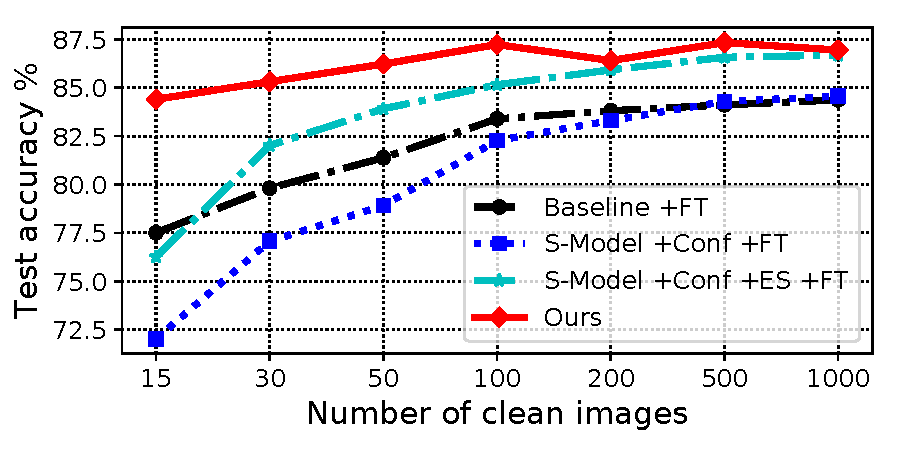
\includegraphics[width=0.9\columnwidth]{figures/cifar-imbalance-ft.pdf}
\fi
\vspace{-0.1in}
\caption{Effect of the number of clean imaged used, on CIFAR-10 with 40\% of data flipped to label 3. ``ES'' denotes early stopping.}
\label{fig:ft}
\end{figure}

% !TEX root = ../main.tex

\begin{figure}[t]
\centering
\iflatexml
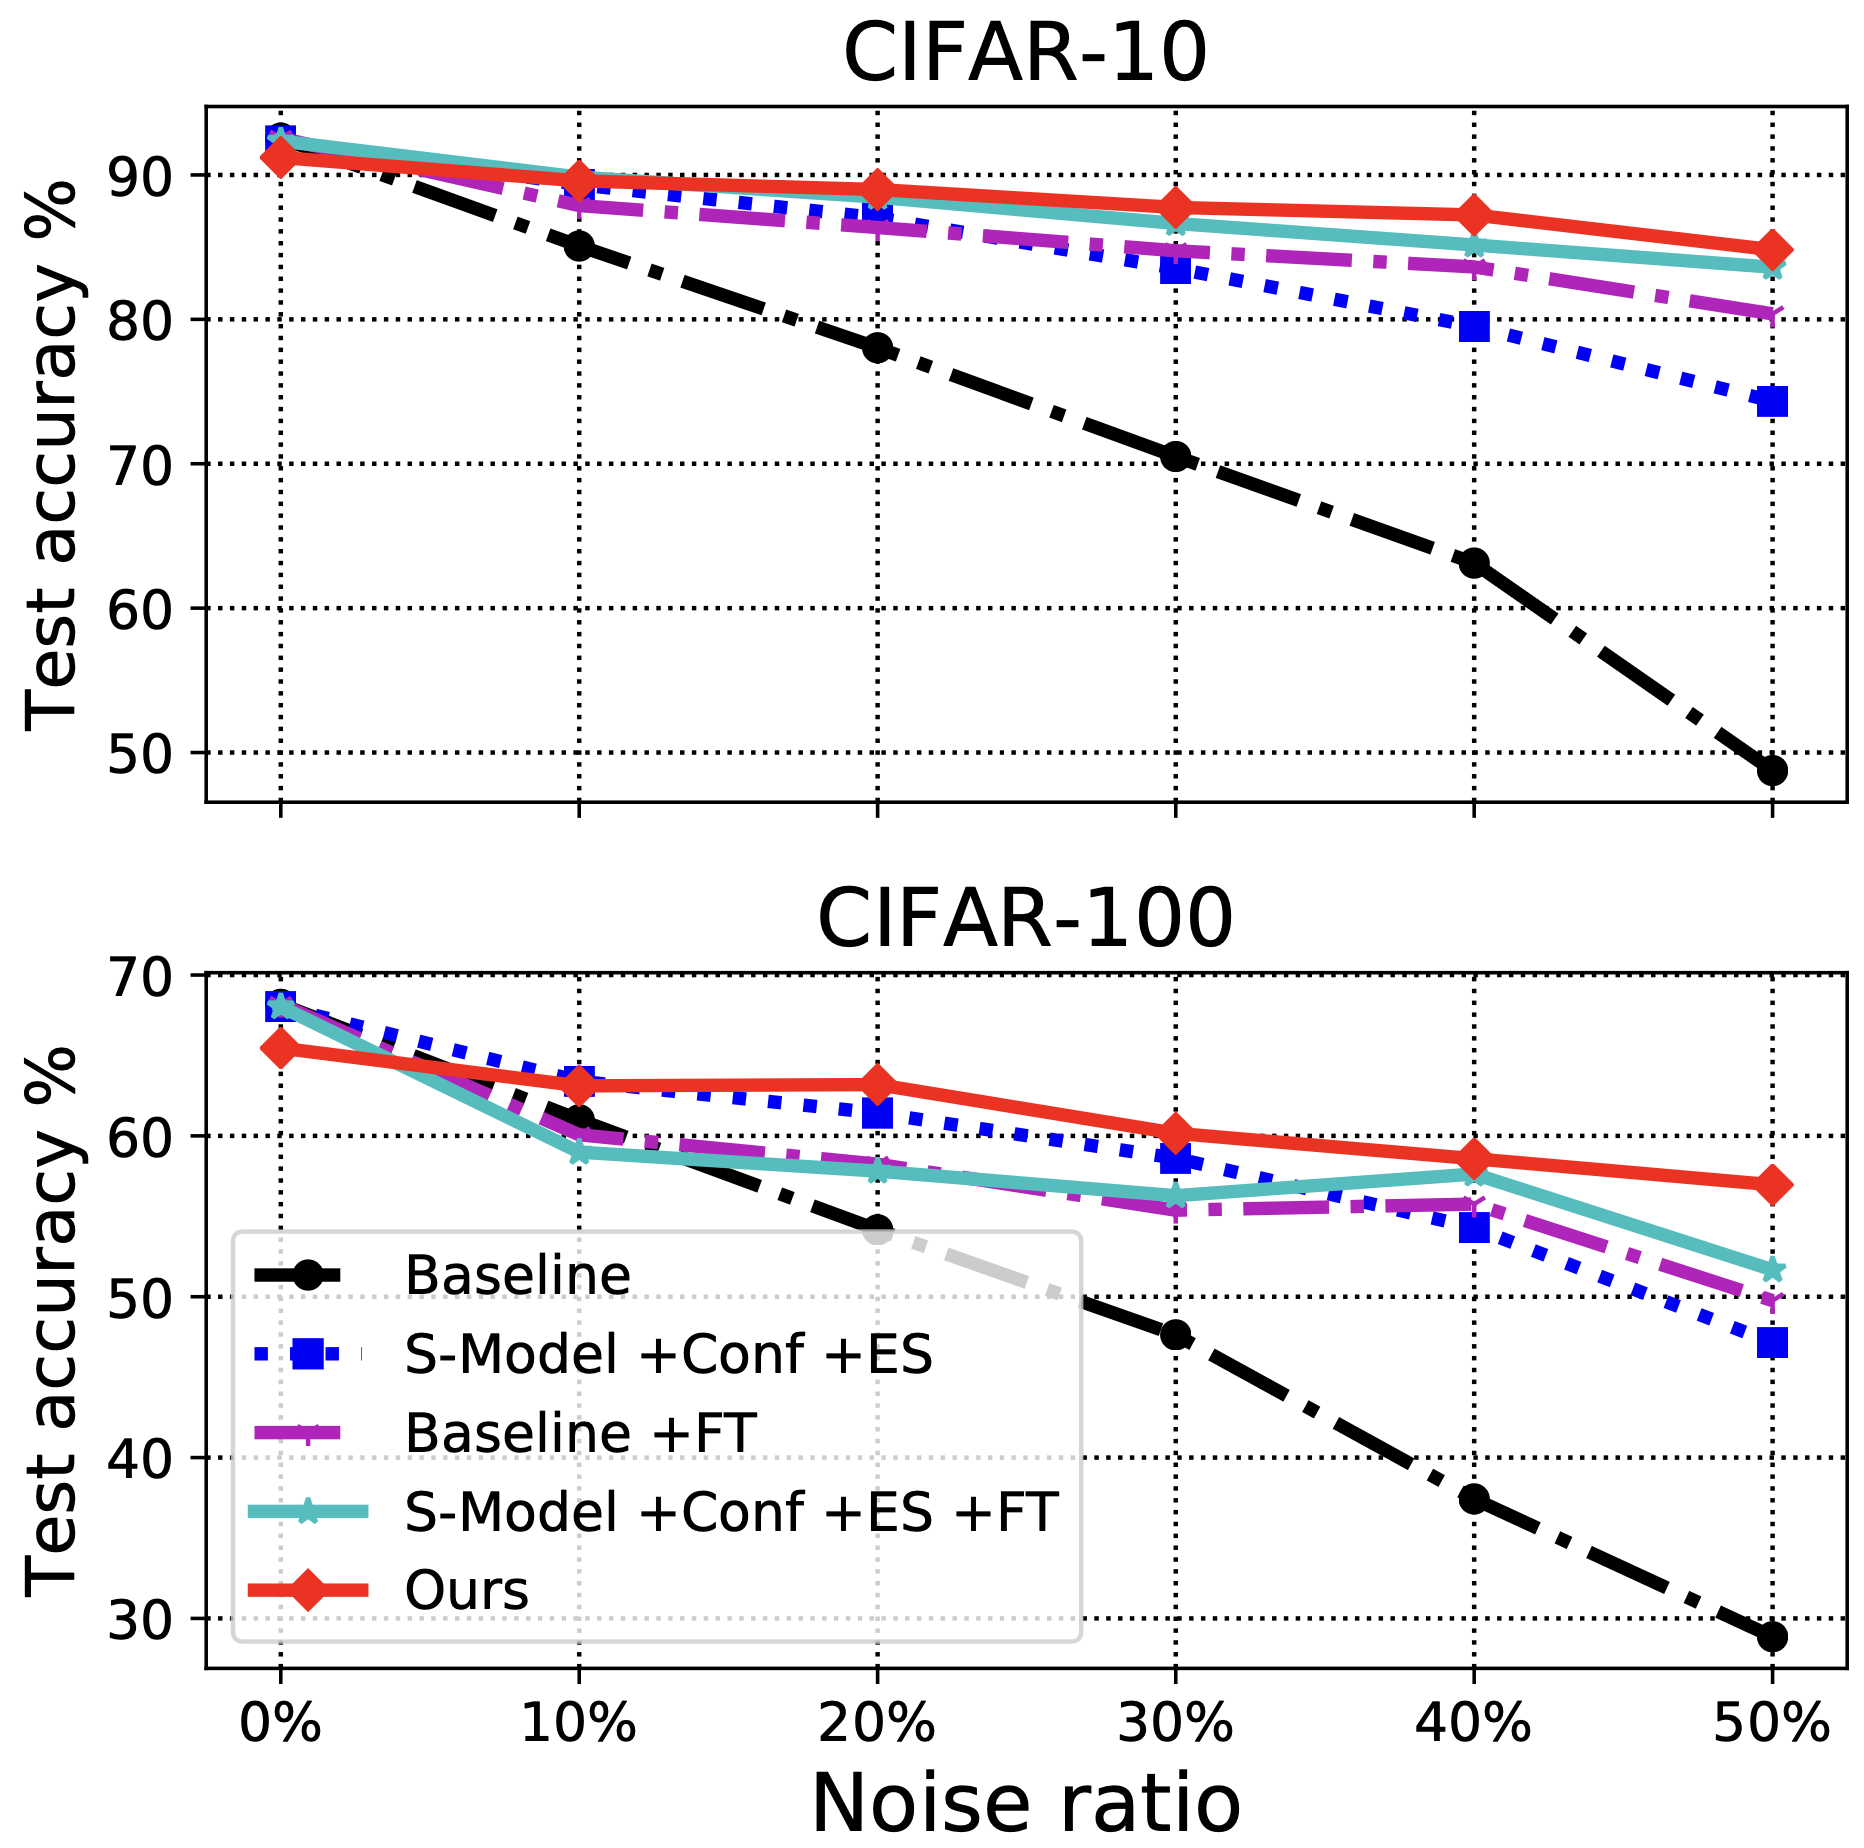
\includegraphics[width=6\columnwidth]{figures/cifar-noisy-imbalance-level.png}
\else
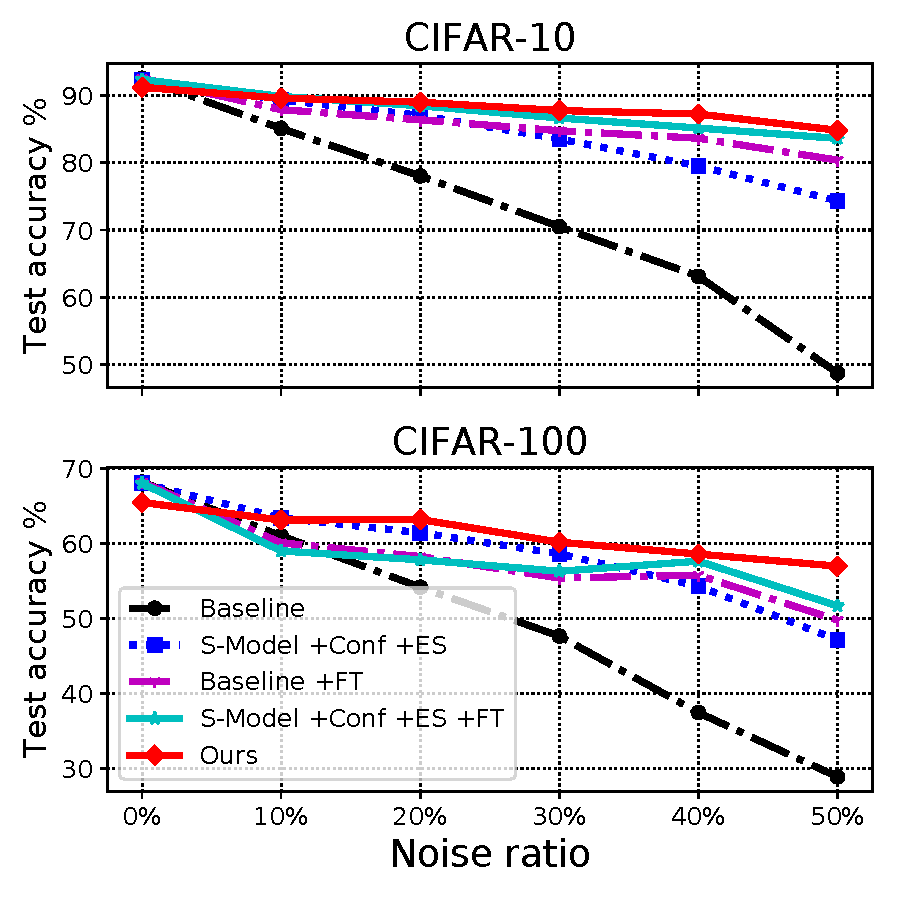
\includegraphics[width=0.9\columnwidth]{figures/cifar-noisy-imbalance-level.pdf}
\fi
\vspace{-0.1in}

\caption{Model test accuracy on imbalanced noisy CIFAR experiments across various noise levels using
a base ResNet-32 model. ``ES'' denotes early stopping, and ``FT'' denotes finetuning.}
\label{fig:level}

\end{figure}

% !TEX root = ../main.tex
\begin{figure}[h!]
\centering
\vspace{-0.1in}
\iflatexml
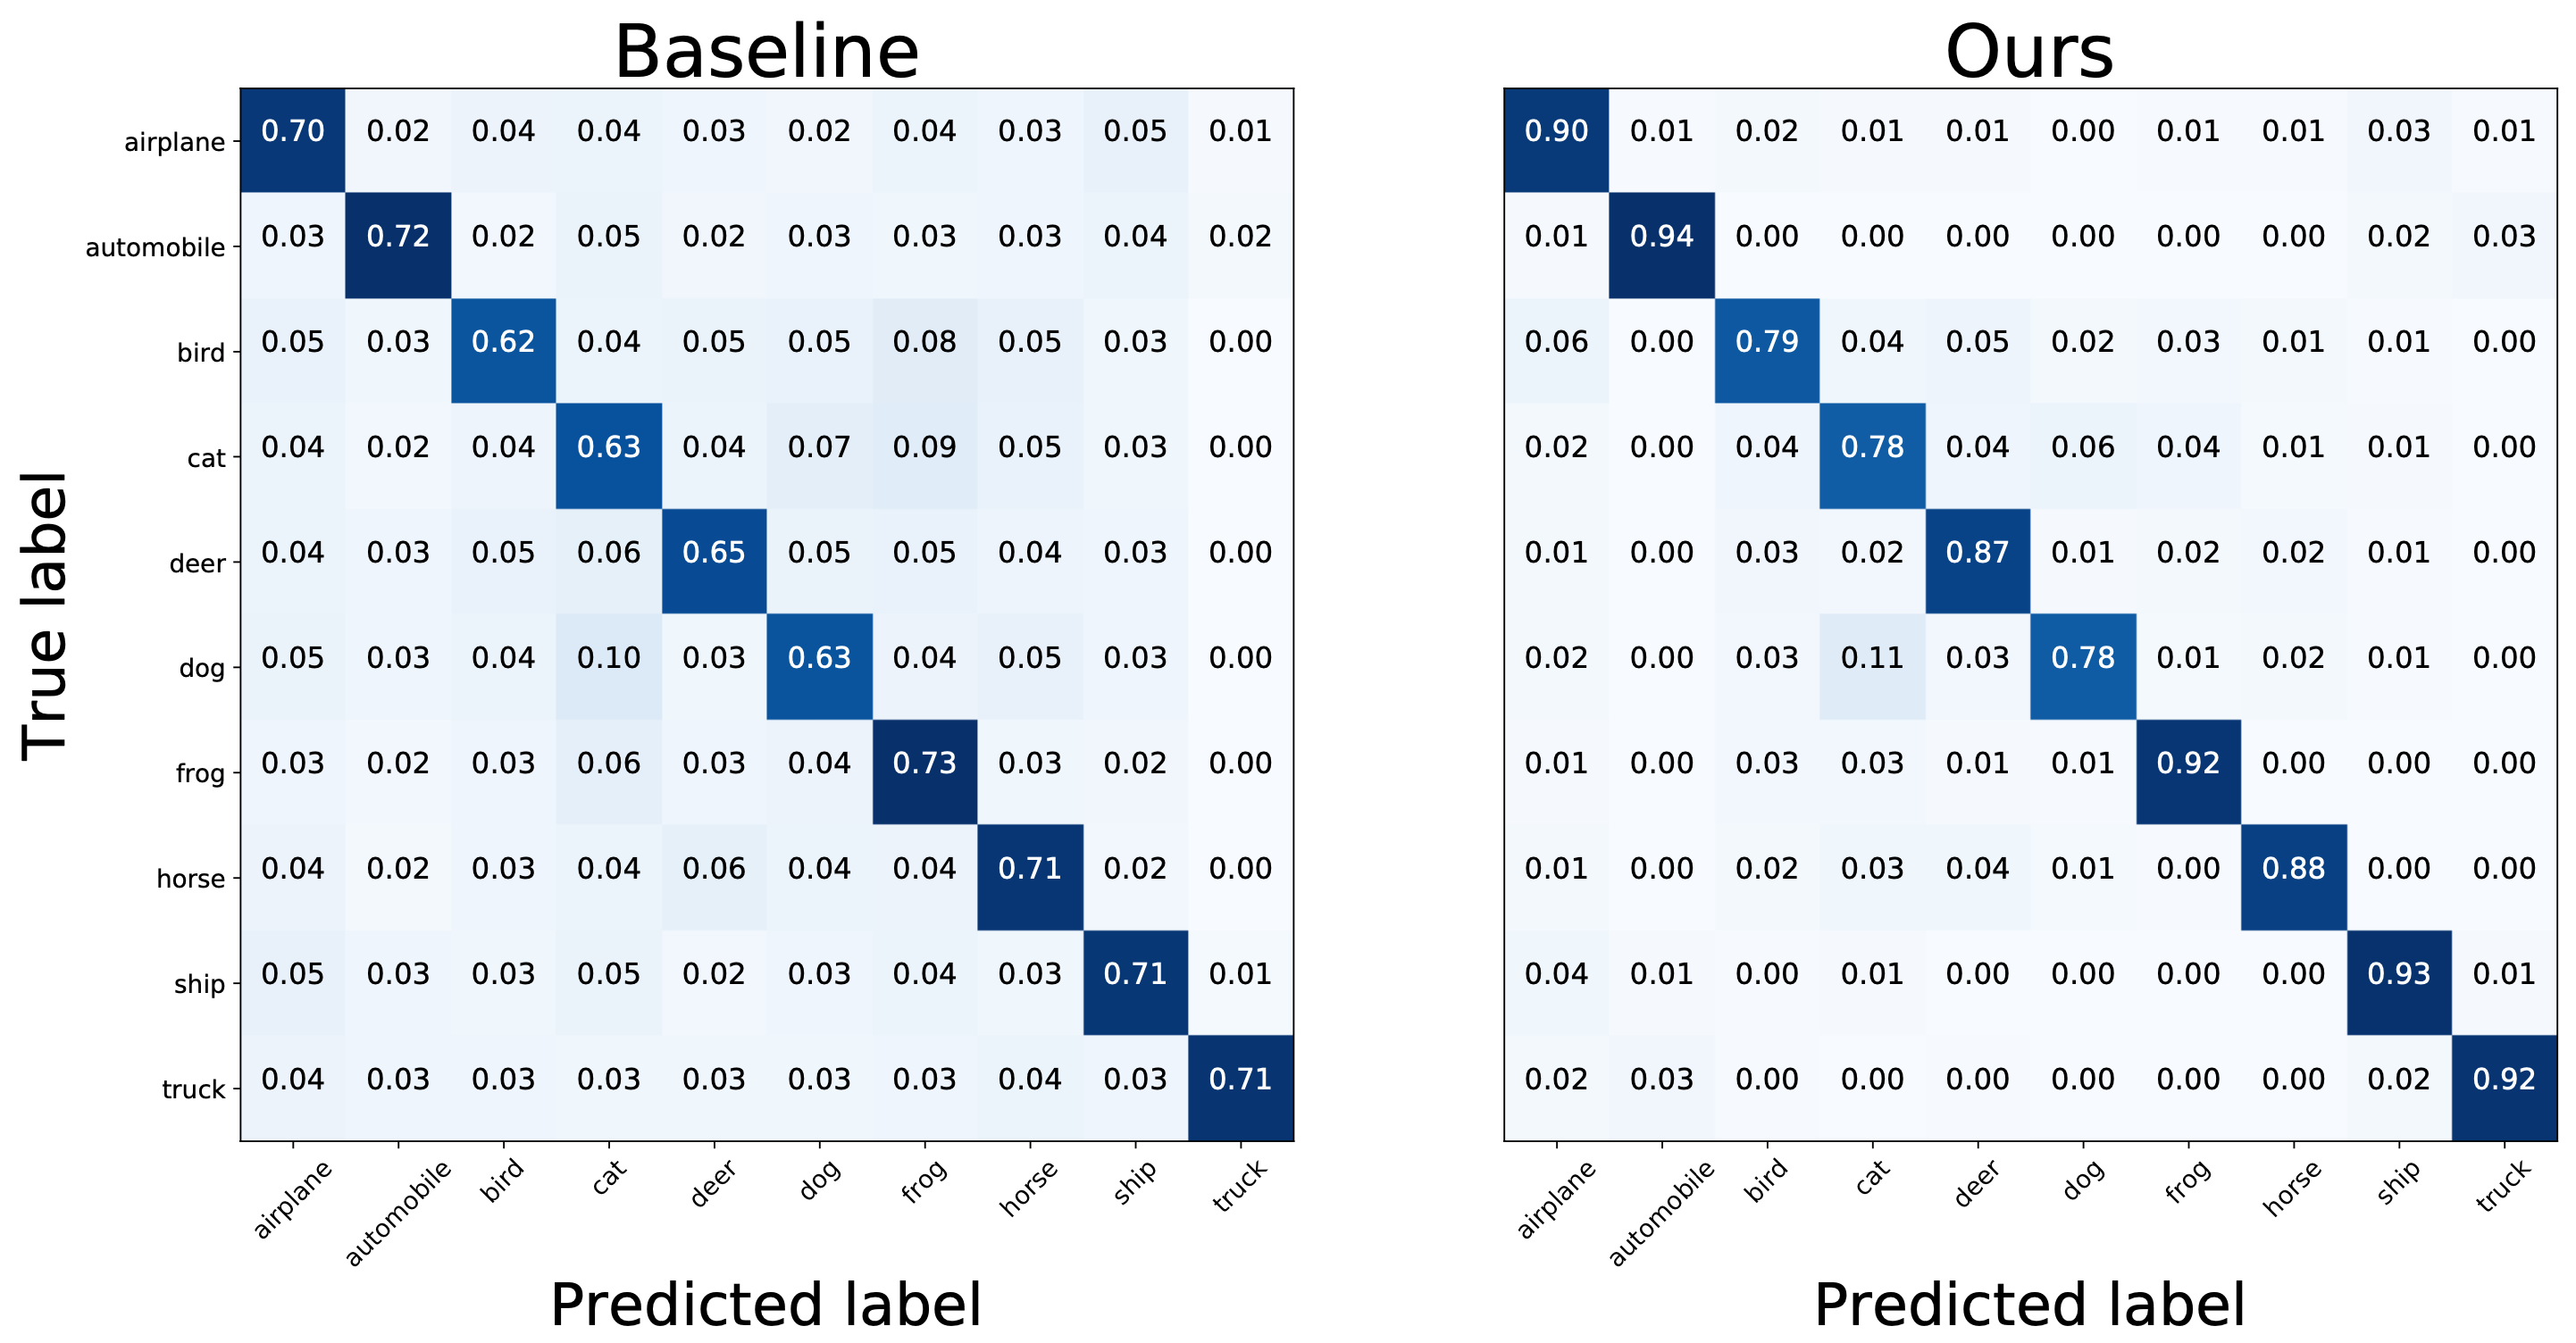
\includegraphics[width=3\columnwidth]{figures/cifar-noise-cm.png}
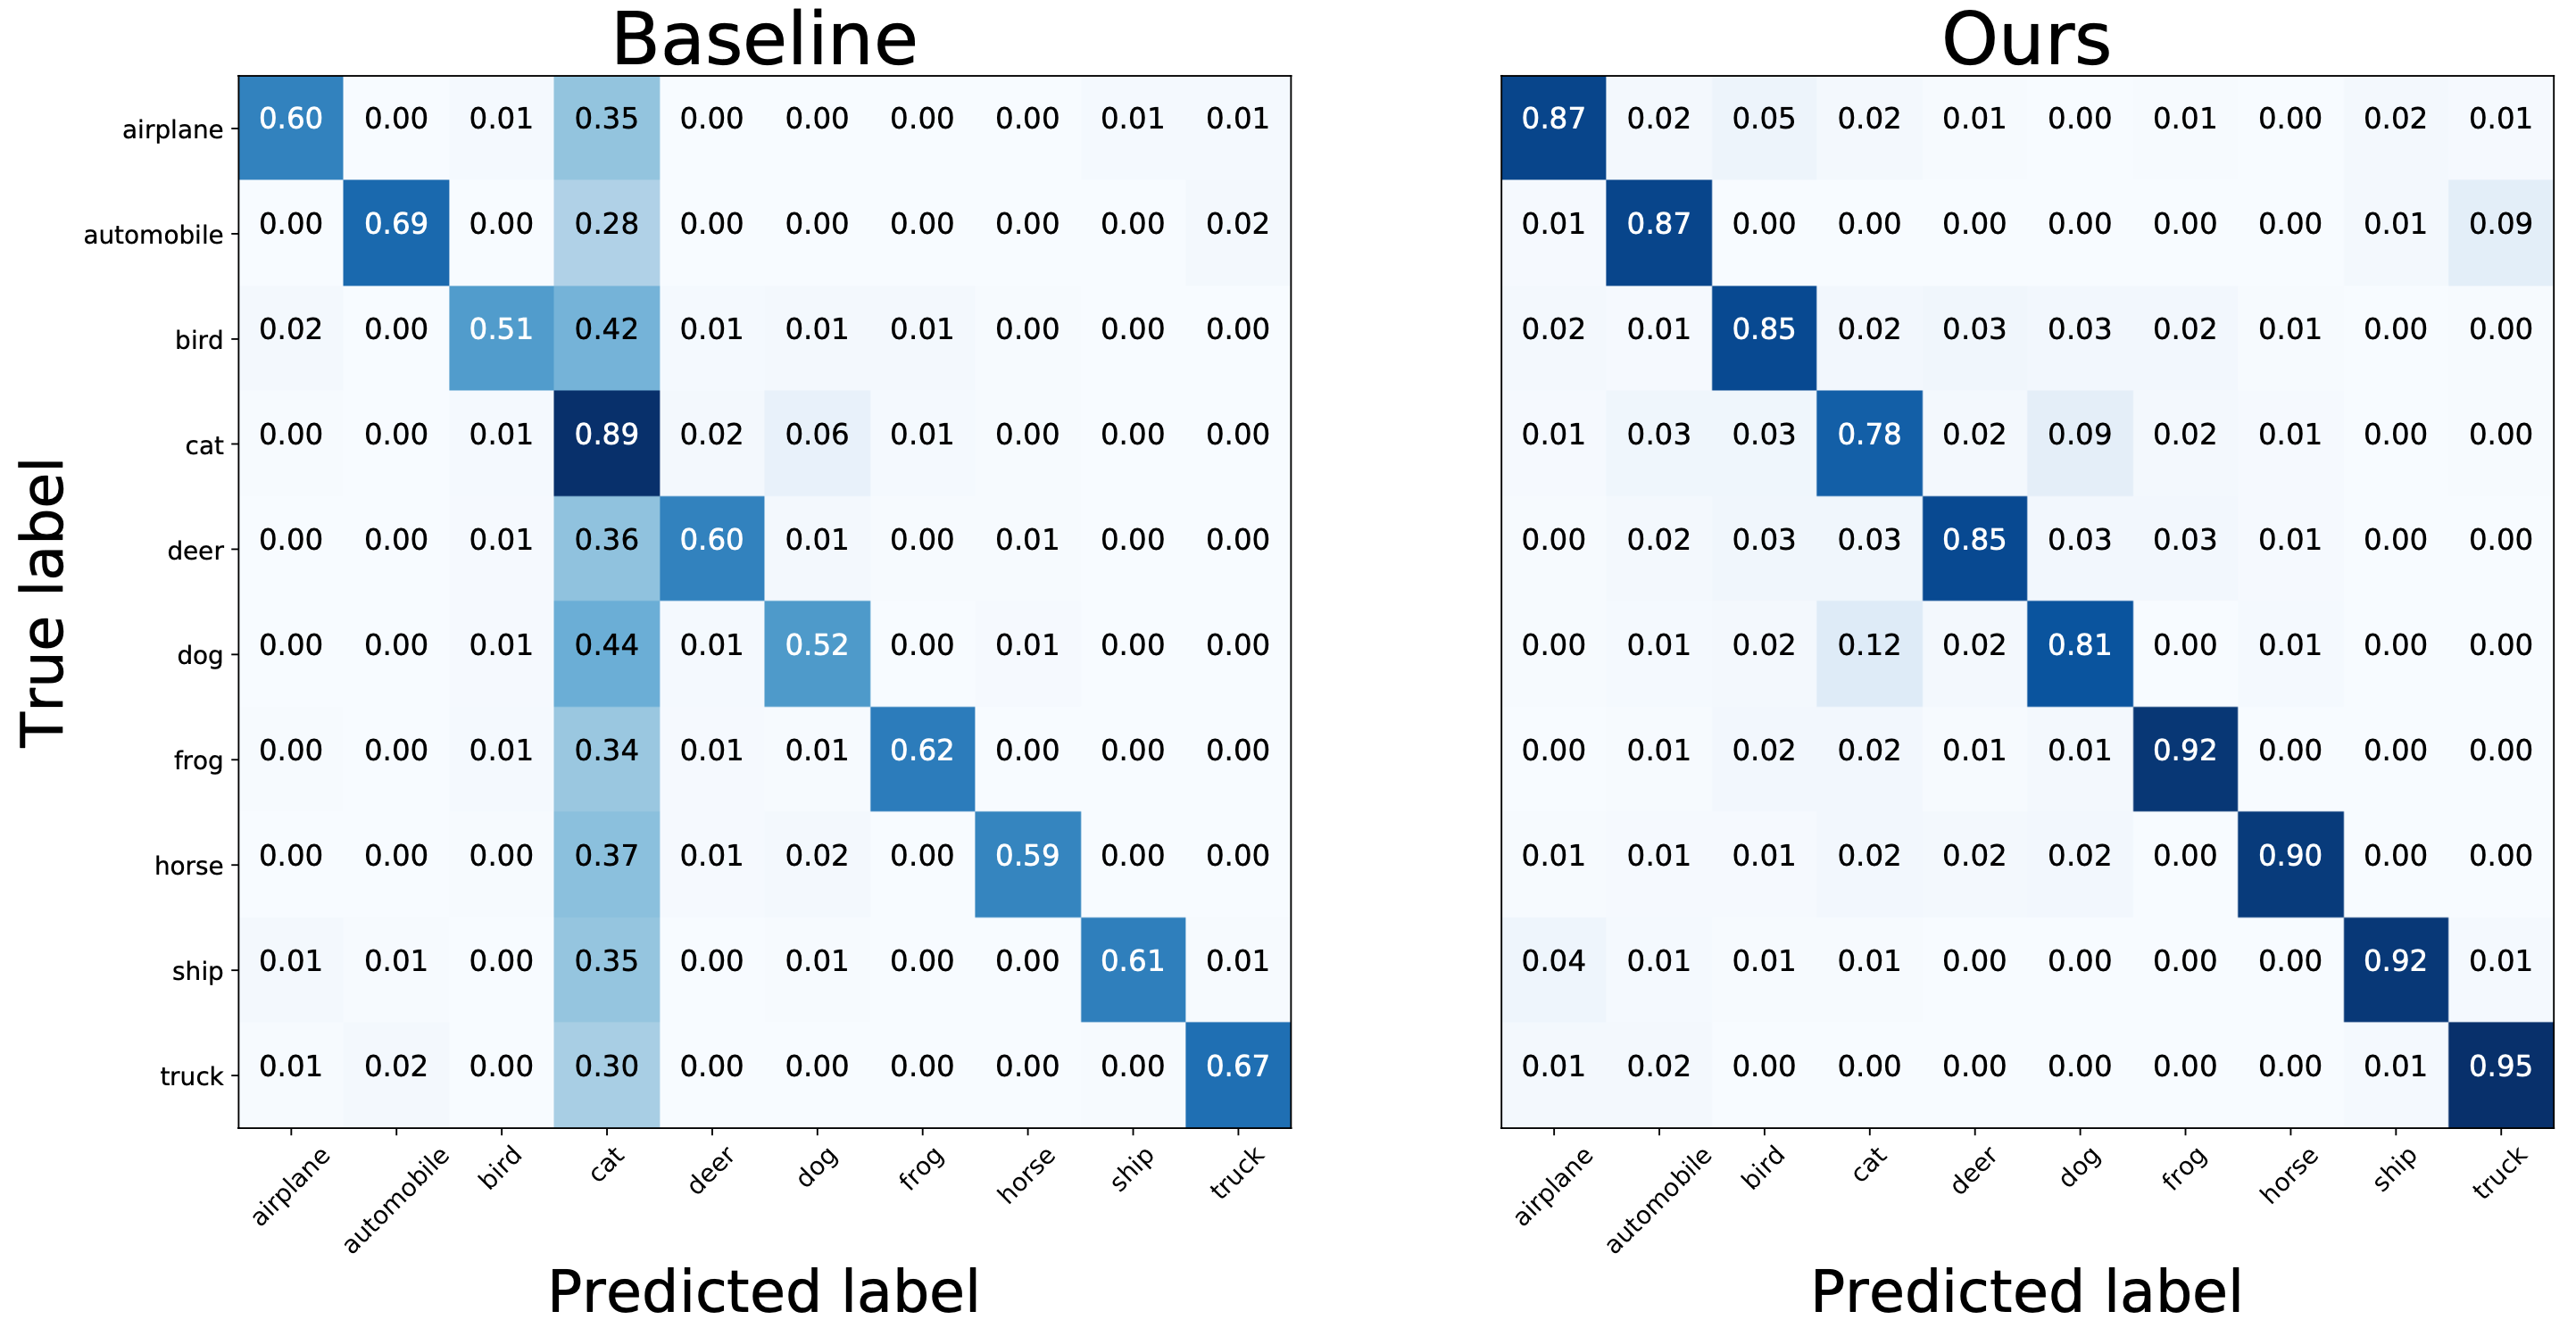
\includegraphics[width=3\columnwidth]{figures/cifar-imbalance-cm.png}
\else
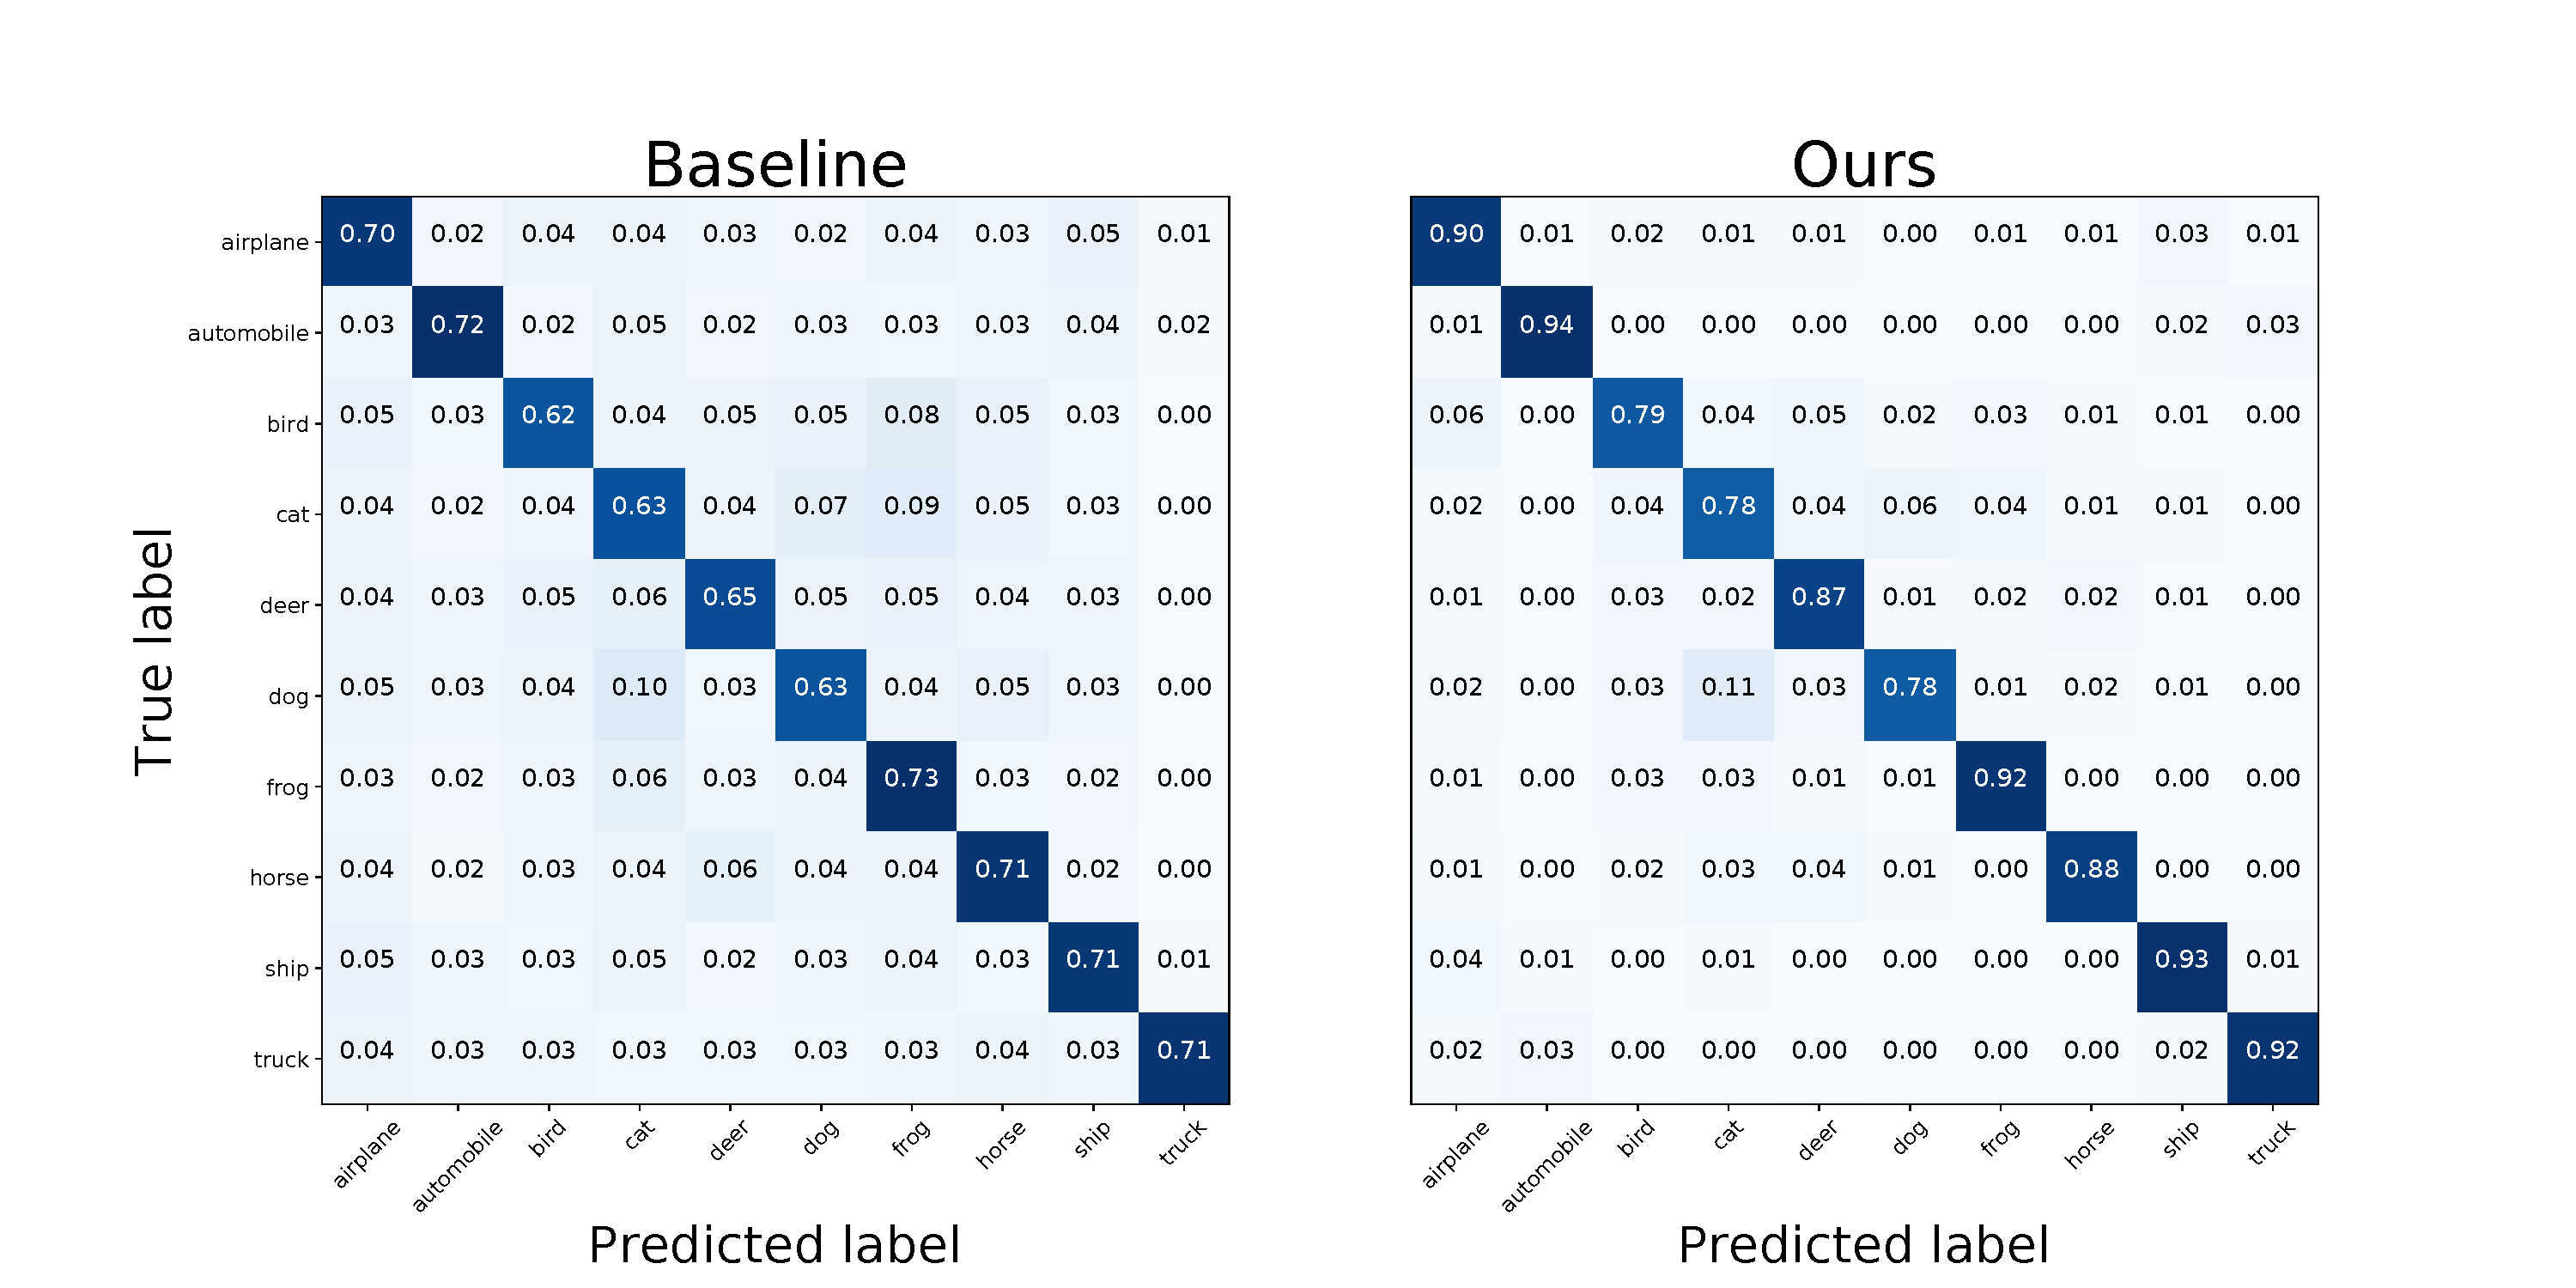
\includegraphics[width=\columnwidth,trim={2.5cm 0 4cm 0},clip]{figures/cifar-noise-cm.pdf}
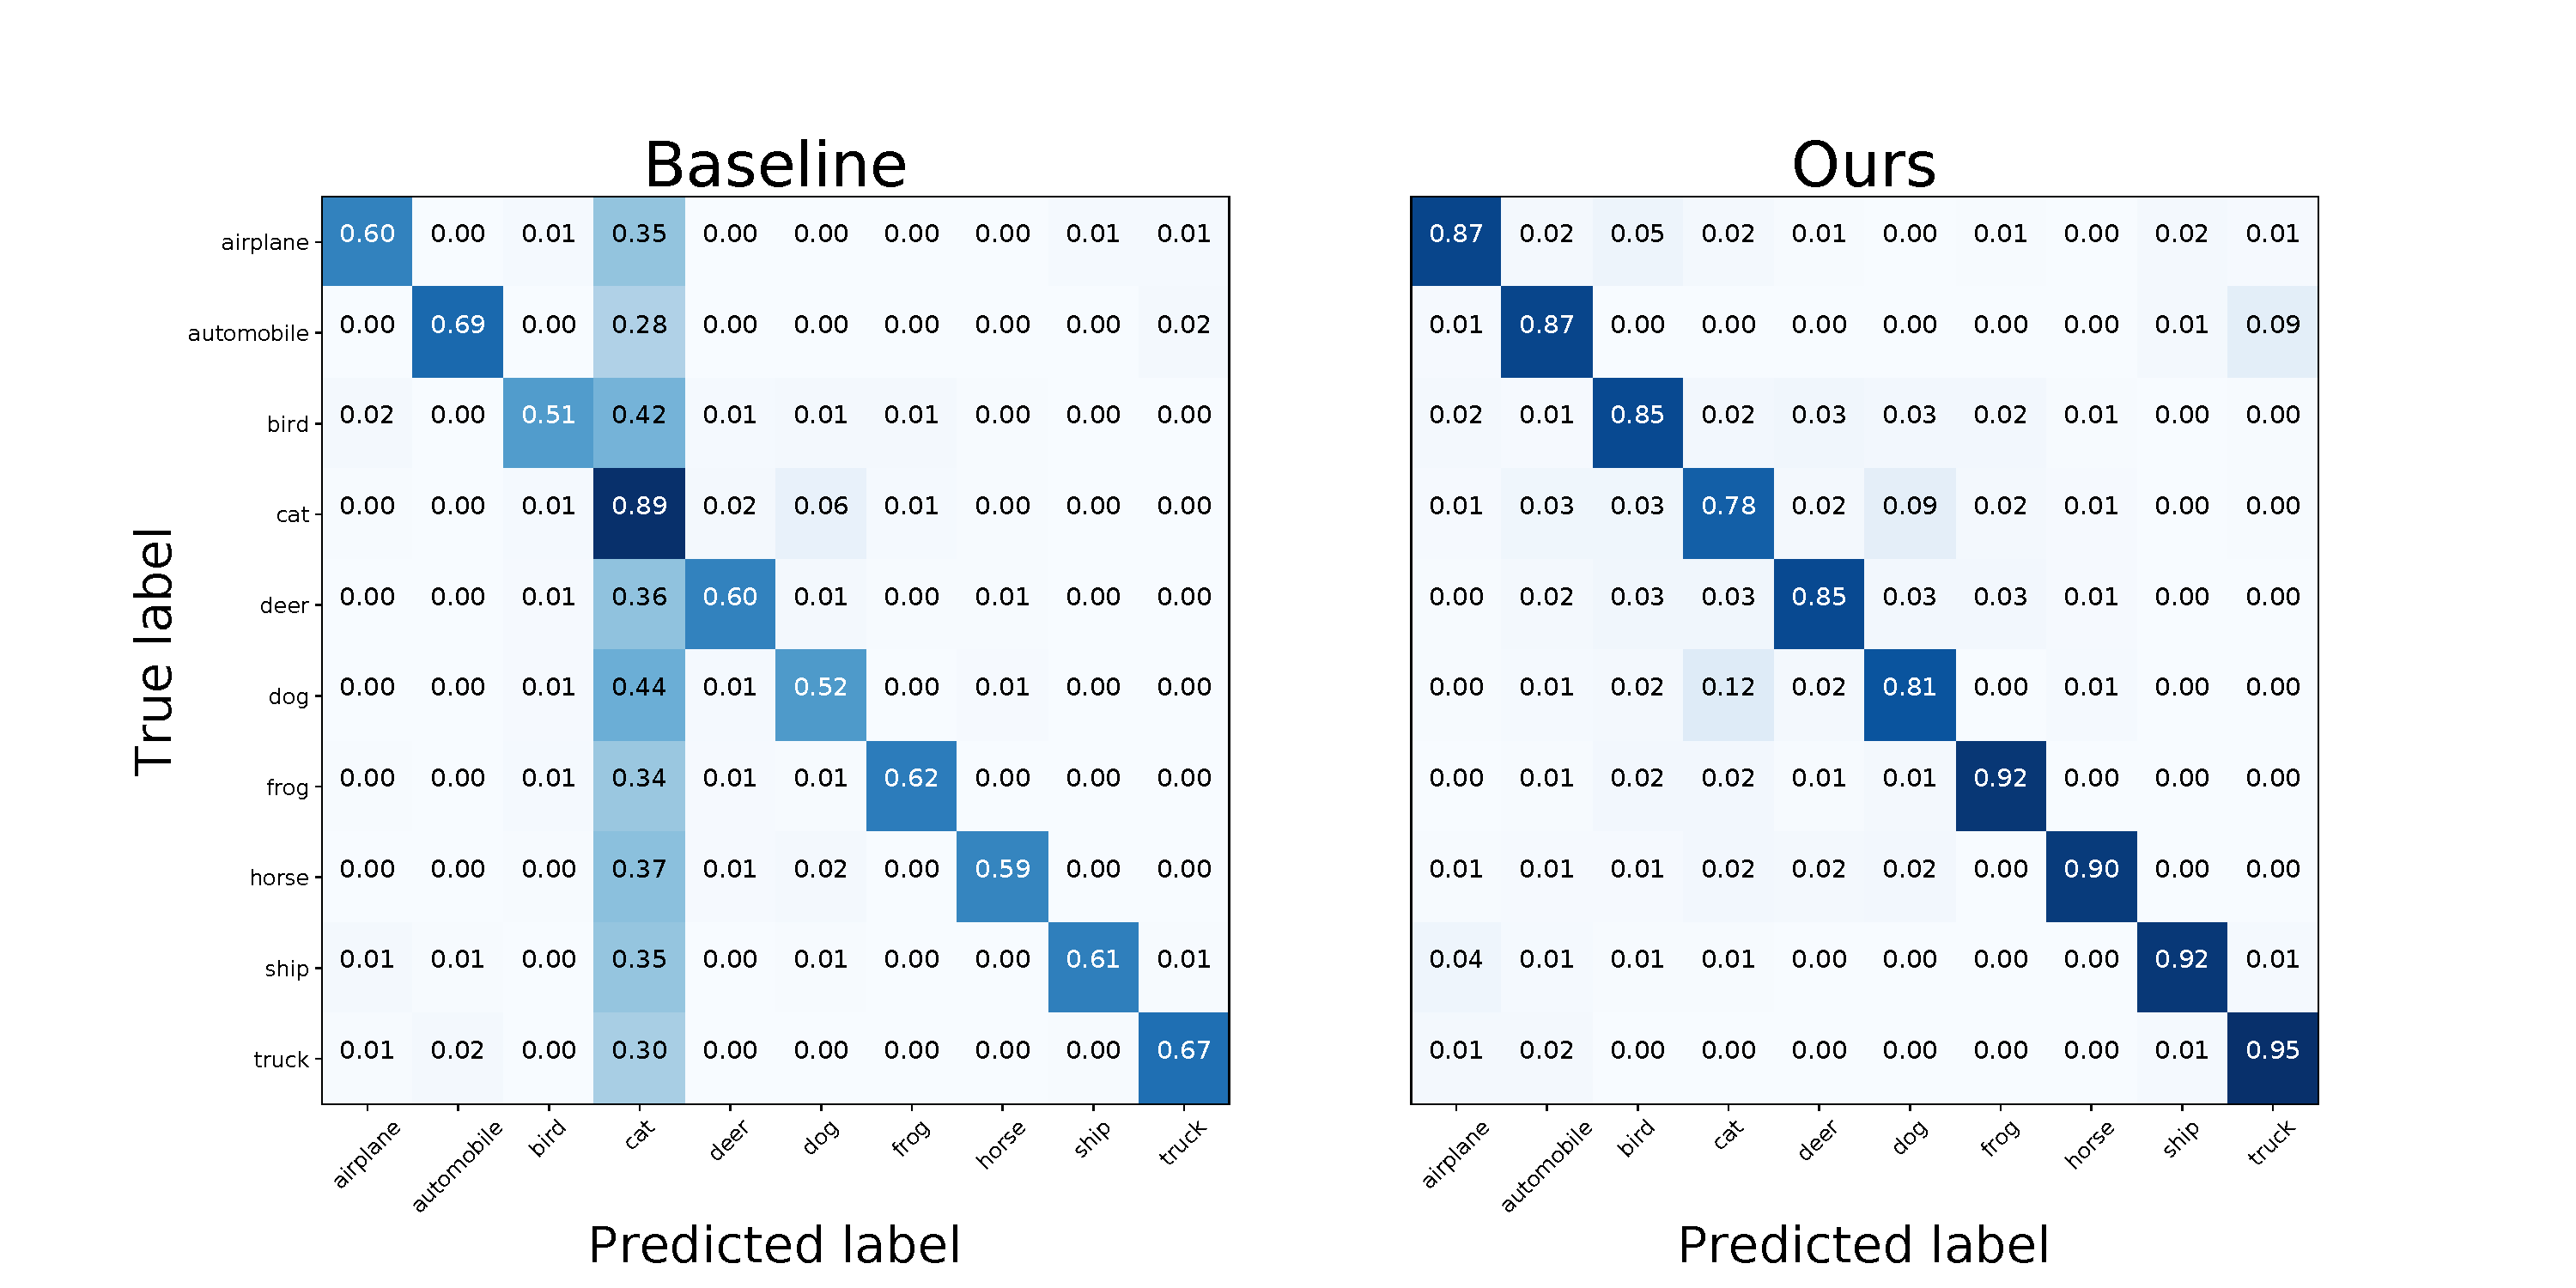
\includegraphics[width=\columnwidth,trim={2.5cm 0 4cm 0},clip]{figures/cifar-imbalance-cm.pdf}
\fi
\vspace{-0.2in}
\iflatexml
\caption{Confusion matrices on CIFAR-10 \textsc{UniformFlip} (left) and \textsc{BackgroundFlip} (right)}
\else
\caption{Confusion matrices on CIFAR-10 \textsc{UniformFlip} (top) and \textsc{BackgroundFlip} (bottom)}
\fi
\label{fig:confusion}
\vspace{-0.1in}
\end{figure}

% !TEX root = ../main.tex
\begin{figure}[h]
\centering
\iflatexml
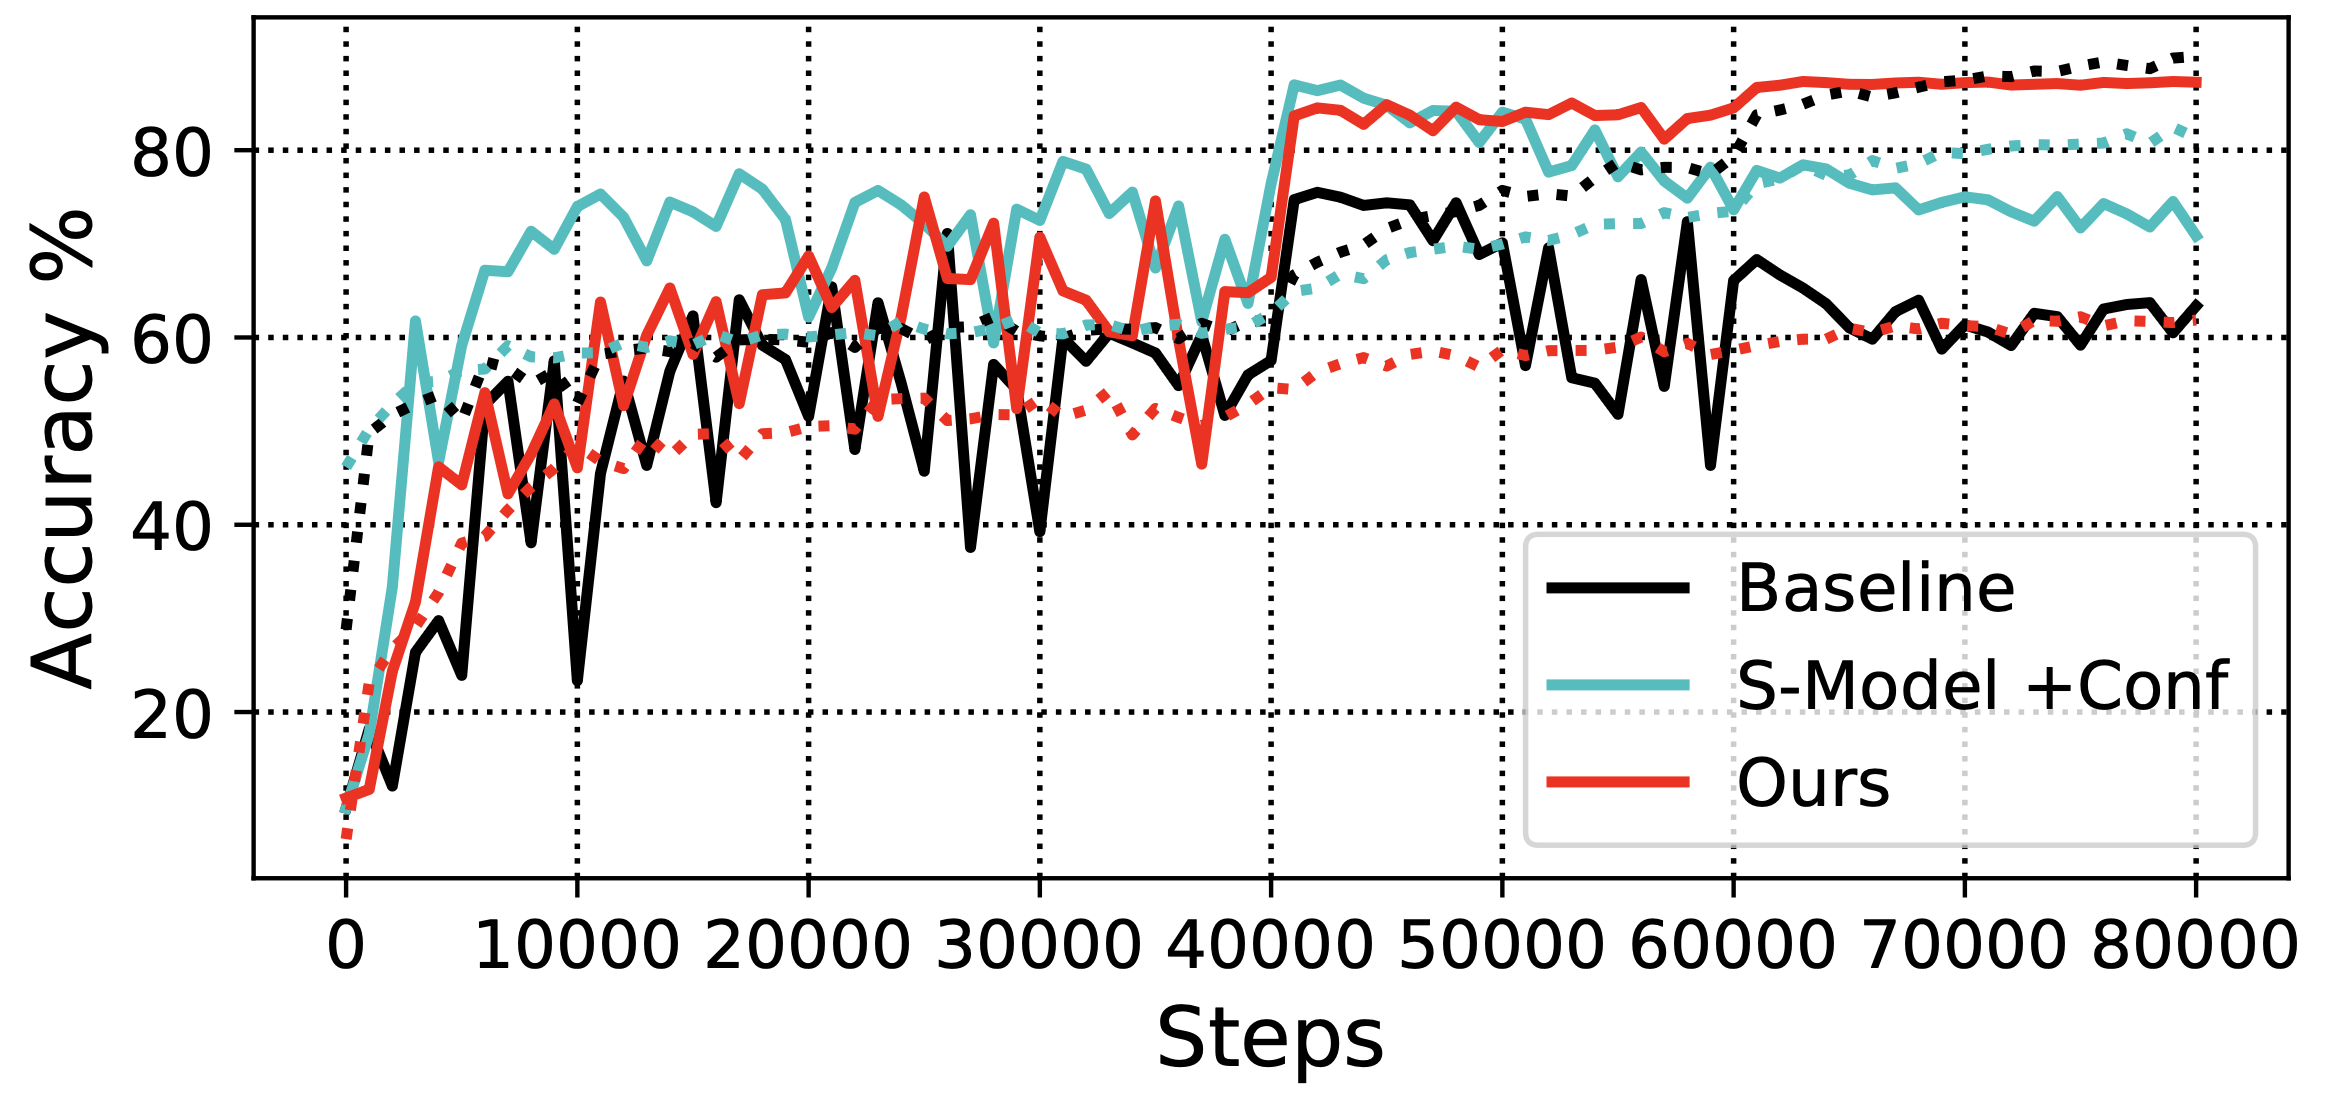
\includegraphics[width=6\columnwidth]{figures/cifar-10-curve.png}
\else
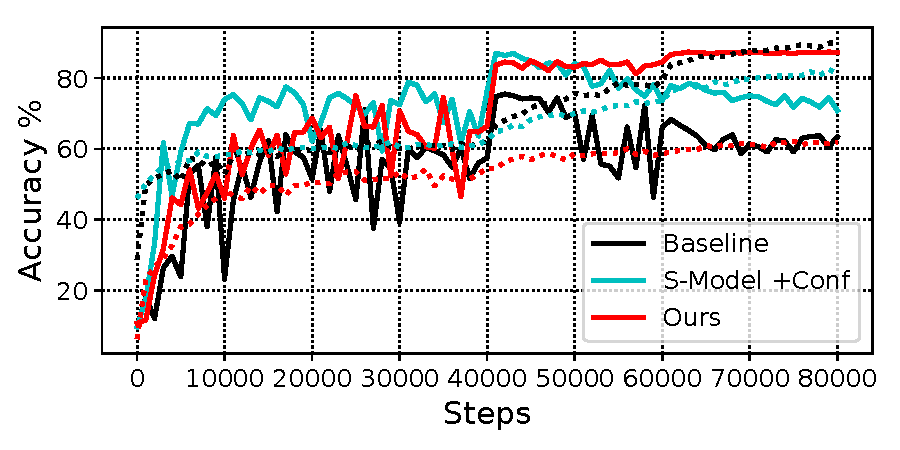
\includegraphics[width=0.9\columnwidth]{figures/cifar-10-curve.pdf}
\fi
\vspace{-0.1in}
\caption{Training curve of a ResNet-32 on CIFAR-10 \textsc{BackgroundFlip} under 40\% noise ratio.
Solid lines denote validation accuracy and dotted lines denote training. Our method is less prone to
label noise overfitting.}
\label{fig:curve}
\vspace{-0.15in}
\end{figure}


\subsection{Results and Discussion}

The first result that draws our attention is that ``Random'' performs surprisingly well on the
\textsc{UniformFlip} benchmark, outperforming all historical methods that we compared. Given that
its performance is comparable with Baseline on \textsc{BackgroundFlip} and MNIST class imbalance, we
hypothesize that random example weights act as a strong regularizer and under which the learning
objective on \textsc{UniformFlip} is still consistent.

Regardless of the strong baseline, our method ranks the top on both \textsc{UniformFlip} and
\textsc{BackgroundFlip}, showing our method is less affected by the changes in the noise type. On
CIFAR-100, our method wins more than 3\% compared to the state-of-the-art method.
\vspace{-0.05in}
\paragraph{Understanding the reweighting mechanism}
It is beneficial to understand how our reweighting algorithm contributes to learning more robust
models during training. First, we use a pre-trained model (trained at half of the total iterations
without learning rate decay) and measure the example weight distribution of a randomly sampled batch
of validation images, which the model has never seen. As shown in the left figure of Figure
\ref{fig:dist}, our model correctly pushes most noisy images to zero weights. Secondly,  we
conditioned the input mini-batch to be a single non-background class and randomly flip 40\% of the
images to the background, and we would like to see how well our model can distinguish clean and
noisy images. As shown in Figure \ref{fig:dist} right, the model is able to reliably detect images
that are flipped to the background class.
\vspace{-0.05in}
\paragraph{Robustness to overfitting noise} Throughout experimentation, we find baseline
models can easily overfit to the noise in the training set. For example, shown in
Table~\ref{tab:backgroundflip}, applying early stopping (``ES'') helps the classification
performance of ``S-Model'' by over 10\% on CIFAR-10. Figure~\ref{fig:confusion} compares the final
confusion matrices of the baseline and the proposed algorithm, where a large proportion of noise
transition probability is cleared in the final prediction. Figure~\ref{fig:curve} shows training
curves on the \textsc{BackgroundFlip} experiments. After the first learning rate decay, both
``Baseline'' and ``S-Model'' quickly degrade their validation performance due to overfitting, while
our model remains the same validation accuracy until termination. Note that here ``S-Model'' knows
the oracle noise ratio in each class, and this information is not available in our method.
\vspace{-0.05in}
\paragraph{Impact of the noise level} We would like to investigate how strongly our method can
perform on a variety of noise levels. Shown in Figure~\ref{fig:level}, our method only drops 6\%
accuracy when the noise ratio increased from 0\% to 50\%; whereas the baseline has dropped more than
40\%. At 0\% noise, our method only slightly underperforms baseline. This is reasonable since we are
optimizing on the validation set, which is strictly a subset of the full training set, and therefore
suffers from its own subsample bias.
\vspace{-0.05in}
\paragraph{Size of the clean validation set} When the size of the clean validation set grows larger,
fine-tuning on the validation set will be a reasonble approach. Here, we make an attempt to explore
the tradeoff and understand when fine-tuning becomes beneficial. Figure~\ref{fig:ft} plots the
classification performance when we varied the size of the clean validation on
\textsc{BackgroundFlip}. Surprisingly, using 15 validation images for all classes only results in a
2\% drop in performance, and the overall classification performance does not grow after having more
than 100 validation images. In comparison, we observe a significant drop in performance when only
fine-tuning on these 15 validation images for the baselines, and the performance catches up around
using 1,000 validation images (100 per class). This phenomenon suggests that in our method the clean
validation acts more like a regularizer rather than a data source for parameter fine-tuning, and
potentially our method can be complementary with fine-tuning based method when the size of the clean
set grows larger.

% !TEX root = ../main.tex
\vspace{-0.1in}
\section{Conclusion}
In this work, we propose an end-to-end learned, sparse visual attention
mechanism for self-driving, where the sparse attention mask gates the feature backbone
computation. As opposed to existing methods that focus on using attention for perception only,
our attention masks are directly optimized for motion planning, which enables our network to output
better planned trajectories while achieving more efficiency with higher sparsity. In future work,
the attention module can be extended to have recurrent feedbacks from the output layers
to better leverage temporal information.


\let\oldbibliography\thebibliography
\renewcommand{\thebibliography}[1]{\oldbibliography{#1}
\setlength{\itemsep}{7pt}} %Reducing spacing in the bibliography.

% \newpage
\bibliography{our_ref}
\bibliographystyle{icml2018}
% \bibliographystyle{iclr2023_conference}

\if\arxiv1
\newpage
% !TEX root = ../main.tex
\section{Dataset Details}
\label{app:data}

\subsection{Benchmark comparison}
We include Table~\ref{tab:benchmark} to compare existing continual and few-shot learning paradigms.

\subsection{\ourchar{} \& \ourimg{} Sampler Details}
For the \ourchar{} and the \ourimg{} experiments, we use sequences with maximum 150 images, from 5 environments. For
individual environment, we use a Chinese restaurant process to sample the class distribution. In
particular, the probability of sampling a new class is:
\begin{align}
p_\text{new} = \frac{k \alpha + \theta}{m + \theta},
\end{align}
where $k$ is the number of classes that we have already sampled in the environment, and $m$ is the
total number of instances we have in the environment. $\alpha$ is set to 0.2 and $\theta$ is set to
1.0 in all experiments.

The environment switching is implemented by a Markov switching process. At each step in the
sequence there is a constant probability $p_\text{switch}$ that switches to another environment. For
all experiments, we set $p_\text{switch}$ to 0.2. We truncate the maximum number of appearances
per class to 6. If the maximum appearance is reached, we will sample another class.

\subsection{Metrics}
\label{sec:metrics}
\paragraph{Average precision:} We chose to use AP (average precision or area under the precision-recall curve) as a way of integrating two aspects of performance:

\begin{enumerate}
    \item the binary accuracy of whether an instance belongs to a known or unknown class (KU-Assign for short), and
    \item the accuracy of assigning an instance the correct class label given it is from a known class (Class-Assign for short).
\end{enumerate}
The procedure to calculate AP is as follows. We first sort all the {KU-Assign, Class-Assign} predictions across all sequences in descending order based on KU-Assign probability, where the high ranked predictions should be known (not novel) classes. For the N top ranked instances in the sorted list, we compute:
\begin{enumerate}
    \item precision@N = correct(Class-Assign)@N / N
    \item recall@N = correct(Class-Assign)@N / K,
\end{enumerate}
where K is the true number of known instances and correct(Class-Assign)@N is the count of the number of correct class assignments among the top N. (The class assignment for an unknown instance is always incorrect.) To obtain the AP, we compute the integral of the function (y=precision@N, x=recall@N) across all N’s.

\paragraph{N-shot accuracy:} We define N-shot accuracy as the number of times an instance that has been seen N times thus far in the sequence is classified correctly. We compute the mean and standard error of this over all sequences.

\subsection{Additional \ourroom{} Statistics} 
Statistics of the \ourroom{} are included in Table~\ref{tab:dataset_stats}, in comparison to other
few-shot and continual learning datasets. Note that since \ourroom{} is collected from a simulated
environment, with 90 indoor worlds consisting of 1.2K panorama images and 1.22M video frames. The
dataset contains about 6.9K random walk sequences with a maximum of 200 frames per sequence. For
training we randomly crop 100 frames to form a training sequence. There are 7.0K unique instance
classes.

Plots of additional statistics of \ourroom{} are shown in Figure~\ref{fig:additionalstats}. In
addition to the ones shown in the main paper, instances and viewpoints also follow long tail
distributions. The number of objects in each frame follows an exponential distribution.

% !TEX root = ../main.tex
\begin{table}[t]
\iflatexml
    \begin{tabular}{ccccccc}
    \toprule
                                  & {\bf Images} & {\bf Sequences} & {\bf Classes} & {\bf Content}                  \\
    \midrule                                                                     
    Permuted MNIST~\citep{mnist}   & 60K          & -           & -          & Hand written digits          \\
    Omniglot~\citep{omniglot}      & 32.4K        & -           & 1.6K       & Hand written characters      \\
    CIFAR-100~\citep{cifar}        & 50K          & -           & 100        & Common objects               \\
    mini-ImageNet~\citep{matchingnet}& 50K        & -           & 100        & Common objects               \\
    tiered-ImageNet~\citep{fewshotssl}& 779K      & -           & 608        & Common objects               \\
    OpenLORIS  \citep{openloris}   & 98K          & -           & 69         & Small table-top obj.         \\
    CORe50  \citep{core50}         & 164.8K       & 11          & 50         & Hand-held obj.               \\
    \midrule                                                                                                          
    \ourroom{} (Ours)            & 1.22M         & 6.9K        & 7.0K       & General indoor instances     \\
    \bottomrule
    \end{tabular}
    \caption{\small Continual \& few-shot learning datasets}
    \label{tab:dataset_stats}
\else
    \vspace{-0.5in}
    \begin{center}
    \begin{small}
    \caption{\small Continual \& few-shot learning datasets}
    \label{tab:dataset_stats}
    \begin{tabular}{ccccccc}
    \toprule
                                  & {\bf Images} & {\bf Sequences} & {\bf Classes} & {\bf Content}                  \\
    \midrule                                                                     
    Permuted MNIST~\citep{mnist}   & 60K          & -           & -          & Hand written digits          \\
    Omniglot~\citep{omniglot}      & 32.4K        & -           & 1.6K       & Hand written characters      \\
    CIFAR-100~\citep{cifar}        & 50K          & -           & 100        & Common objects               \\
    mini-ImageNet~\citep{matchingnet}& 50K        & -           & 100        & Common objects               \\
    tiered-ImageNet~\citep{fewshotssl}& 779K      & -           & 608        & Common objects               \\
    OpenLORIS  \citep{openloris}   & 98K          & -           & 69         & Small table-top obj.         \\
    CORe50  \citep{core50}         & 164.8K       & 11          & 50         & Hand-held obj.               \\
    \midrule                                                                                                          
    \ourroom{} (Ours)            & 1.22M         & 6.9K        & 7.0K       & General indoor instances     \\
    \bottomrule
    \end{tabular}
    \vspace{-0.2in}
    \end{small}
    \end{center}
\fi
\end{table}


\subsection{\ourroom{} Simulator Details}
We generate our episodes with a two-stage process using two simulators -- HabitatSim~\citep{habitat}
and MatterSim~\citep{mattersim} -- because HabitatSim is based on 3D meshes and using HabitatSim
alone will result in poor image quality due to incorrect mesh reconstruction. Therefore we
sacrificed the continuous movement of agents within HabitatSim and base our environment navigation
on the discrete viewpoints in MatterSim, which is based on real panoramic images. The horizontal
field of view is set to 90 degrees for HabitatSim and 100 degrees for MatterSim, and we simulate
with\ 800$\times$600 resolution.

The first stage of generation involves randomly picking a sequence of viewpoints on the connectivity
graph within MatterSim. For each viewpoint, the agent scans the environment along the yaw and pitch
axes for a random period of time until a navigable viewpoint is within view. The time spent in a
single viewpoint follows a Gaussian distribution with mean 5.0 and standard deviation 1.0. At the
start of each new viewpoint, the agent randomly picks a direction to rotate and takes 12.5 degree
steps along the yaw axis, and with 95\% probability, a 5 degree rotation along the pitch axis is
applied in a randomly chosen direction. When a navigable viewpoint is detected, the agent will
navigate to the new viewpoint and reset the direction of scan. When multiple navigable viewpoints
are present, the agent uniformly samples one.

In the second stage, an agent in HabitatSim retraces the viewpoint path and movements of the first
stage generated by MatterSim, collecting mesh-rendered RGB and instance segmentation sensor data.
The MatterSim RGB and HabitatSim RGB images are then aligned via FLANN-based feature matching
~\citep{muja2009flann}, resulting in an alignment matrix that is used to place the MatterSim RGB and
HabitatSim instance segmentation maps into alignment. The sequence of these MatterSim RGB and
HabitatSim instance segmentation maps constitute an episode.

We keep objects of the following categories: \texttt{picture, chair, lighting, cushion, table,
plant, chest of drawers, towel, sofa, bed, appliances, stool, tv monitor, clothes, toilet,
fireplace, furniture, bathtub, gym equipment, blinds, board panel}. We initially generate 600 frames
per sequence and remove all the frames with no object. Then we store every 200 image frames into a
separate file.

During training and evaluation, each video sequence is loaded, and for each image we go through each
object present in the image. We create the attention map using the segmentation groundtruth of the
selected object. The attention map and the image together form a \textit{frame} in our model input.
For training, we randomly crop 100 frames from the sequence, and for evaluation we use the first 100
frames for deterministic results.

Please visit our released code repository to download the \ourroom{} dataset.

% !TEX root = ../main.tex
\begin{table*}[t]
\iflatexml
    \begin{tabular}{ccccccc}
    \toprule
    \mr{2}{\tb{Tasks}}                     & \tb{Few}  & \tb{Semi-sup. } & \mr{2}{\tb{Continual}} & \tb{Online} & \tb{Predict}& \tb{Soft Context}  \\
                                           & \tb{Shot} & \tb{Supp. Set}  &                        & \tb{Eval.}  & \tb{New}    & \tb{Switch}        \\
    \midrule                                                                                                                                                                          
    Incremental Learning (IL) \citep{icarl}& \xm       & \xm             & \cm                    & \hx         & \xm         & \xm                \\
    Few-shot (FSL) \citep{matchingnet}     & \cm       & \xm             & \xm                    & \xm         & \xm         & \xm                \\
    Incremental FSL \citep{attnattractor}  & \cm       & \xm             & \hx                    & \xm         & \xm         & \xm                \\
    Cls. Incremental FSL \citep{fscil}     & \cm       & \xm             & \cm                    & \hx         & \xm         & \xm                \\
    Semi-supv. FSL \citep{fewshotssl}      & \cm       & \cm             & \xm                    & \xm         & \cm         & \xm                \\
    MOCA \citep{moca}                      & \cm       & \xm             & \cm                    & \xm         & \xm         & \hx                \\
    Online Mixture \citep{onlinemixture}   & \cm       & \xm             & \cm                    & \xm         & \xm         & \hx                \\
    Online Meta \citep{oml}                & \cm       & \xm             & \cm                    & \xm         & \xm         & \xm                \\
    Continual FSL* \citep{contfsl}         & \cm       & \xm             & \cm                    & \xm         & \xm         & \xm                \\
    OSAKA* \citep{osaka}                   & \cm       & \xm             & \cm                    & \cm         & \hx         & \cm                \\
    \midrule                                                                                                                                                                                         
    OC-FSL (Ours)                          & \cm       & \cm             & \cm                    & \cm         & \cm         & \cm                \\
    \bottomrule
    \end{tabular}
    \caption{Comparison of past FSL and CL paradigms vs. our online contextualized FSL (OC-FSL). * denotes concurrent work.}
    \label{tab:benchmark}
\else
    \vspace{-0.5in}
    \caption{Comparison of past FSL and CL paradigms vs. our online contextualized FSL (OC-FSL).}
    \begin{center}
    \begin{small}
    \resizebox{\textwidth}{!}{
    \begin{tabular}{ccccccc}
    \toprule
    \mr{2}{\tb{Tasks}}                     & \tb{Few}  & \tb{Semi-sup. } & \mr{2}{\tb{Continual}} & \tb{Online} & \tb{Predict}& \tb{Soft Context}  \\
                                           & \tb{Shot} & \tb{Supp. Set}  &                        & \tb{Eval.}  & \tb{New}    & \tb{Switch}        \\
    \midrule                                                                                                                                                                          
    Incremental Learning (IL) \citep{icarl}& \xm       & \xm             & \cm                    & \hx         & \xm         & \xm                \\
    Few-shot (FSL) \citep{matchingnet}     & \cm       & \xm             & \xm                    & \xm         & \xm         & \xm                \\
    Incremental FSL \citep{attnattractor}  & \cm       & \xm             & \hx                    & \xm         & \xm         & \xm                \\
    Cls. Incremental FSL \citep{fscil}     & \cm       & \xm             & \cm                    & \hx         & \xm         & \xm                \\
    Semi-supv. FSL \citep{fewshotssl}      & \cm       & \cm             & \xm                    & \xm         & \cm         & \xm                \\
    MOCA \citep{moca}                      & \cm       & \xm             & \cm                    & \xm         & \xm         & \hx                \\
    Online Mixture \citep{onlinemixture}   & \cm       & \xm             & \cm                    & \xm         & \xm         & \hx                \\
    Online Meta \citep{oml}                & \cm       & \xm             & \cm                    & \xm         & \xm         & \xm                \\
    Continual FSL* \citep{contfsl}         & \cm       & \xm             & \cm                    & \xm         & \xm         & \xm                \\
    OSAKA* \citep{osaka}                   & \cm       & \xm             & \cm                    & \cm         & \hx         & \cm                \\
    \midrule                                                                                                                                                                                         
    OC-FSL (Ours)                          & \cm       & \cm             & \cm                    & \cm         & \cm         & \cm                \\
    \bottomrule
    \end{tabular}
    }
    \label{tab:benchmark}
    \\
    \vspace{0.05in}
    * denotes concurrent work.
    \end{small}
    \end{center}
\fi
\end{table*}

\subsection{Semi-supervised Labels:}
Here we describe how we sample the labeled vs. unlabeled flag for each example in the
semi-supervised sequences in both \ourchar{} and \ourroom{} datasets. Due to the imbalance in our
class distribution (from both the Chinese restaurant process and real data collection), directly
masking the label may bias the model to ignore the rare seen classes. Ideally, we would like to
preserve at least one labeled example for each class. Therefore, we designed the following
procedure.

First, for each class $k$, suppose $m_k$ is the number of examples in the sequence that belong to
the class. Let $\alpha$ be the target label ratio. Then the class-specific label ratio $\alpha_k$
is:
\begin{align}
\alpha_k = (1 - \alpha) \exp(-0.5 (m_k - 1)) + \alpha.
\label{eq:semisup}
\end{align}
We then for each class $k$, we sample a binary Bernoulli sequence based on $\Ber(\alpha_k)$. If a
class has all zeros in the Bernoulli sequence, we flip the flag of one of the instances to 1 to make
sure there is at least one labeled instance for each class.
For all experiments, we set $\alpha = 0.3$.

\subsection{Dataset Splits}
We include details about our dataset splits in Table~\ref{tab:omniglotsplit} and
\ref{tab:matterportsplit}.

\section{Experiment Details}
\label{app:exp}
\subsection{Network Architecture}
For the \ourchar{} experiment we used the common 4-layer CNN for few-shot learning with 64 channels
in each layer, resulting in a 64-d feature vector~\citep{protonet}. For the \ourroom{} experiment we
resize the input to 120$\times$160 and we use the ResNet-12 architecture~\citep{tadam} with
\{32,64,128,256\} channels per block. To represent the feature of the input image with an attention
mask, we concatenate the global average pooled feature with the attention ROI feature, resulting in
a 512d feature vector. For the contextual RNN, in both experiments we used an LSTM~\citep{lstm} with
a 256d hidden state. 

We use a linear layer to map from the output of the RNN to the features and control variables. We
obtain $\gamma^{r,w}$ by adding 1.0 to the linear layer output and then applying the softplus
activation. The bias units for $\beta^{r,w}$ are initialized to 10.0. We
also apply the softplus activation to $\bmm$ from the linear layer output.

% !TEX root = ../main.tex
\begin{table}[t]
\iflatexml
    \begin{tabular}{clll}
    \toprule

    \mr{11}{Train} &
    \texttt{Angelic} &
    \texttt{Grantha} &
    \texttt{N Ko}\\
    & 
    \texttt{Aurek-Besh} &
    \texttt{Japanese (hiragana)} &
    \texttt{Malay}
    \\
    & 
    \texttt{Asomtavruli} &
    \texttt{Sanskrit} &
    \texttt{Ojibwe}
    \\
    & 
    \texttt{Korean} &
    \texttt{Arcadian} &
    \texttt{Greek}
    \\
    & 
    \texttt{Alphabet of the Magi} &
    \texttt{Blackfoot} &
    \texttt{Futurama}
    \\
    & 
    \texttt{Tagalog} &
    \texttt{Anglo-Saxon Futhorc} &
    \texttt{Braille}
    \\
    & 
    \texttt{Cyrillic} &
    \texttt{Burmese} &
    \texttt{Avesta}
    \\
    & 
    \texttt{Gujarati} &
    \texttt{Ge ez} &
    \texttt{Syriac (Estrangelo)}
    \\
    & 
    \texttt{Atlantean} &
    \texttt{Japanese (katakana)} &
    \texttt{Balinese}
    \\
    & 
    \texttt{Atemayar Qelisayer} &
    \texttt{Glagolitic} &
    \texttt{Tifinagh}
    \\
    & 
    \texttt{Latin} &
    \texttt{Inuktitut} &
    \\
    \midrule
    \mr{2}{Val} &
    \texttt{Hebrew} &
    \texttt{Mkhedruli} &
    \texttt{Armenian}\\
    & 
    \texttt{Early Aramaic} &
    \texttt{Bengali} &
    \\
    \midrule

    \mr{5}{Test} & 
    \texttt{Gurmukhi} &
    \texttt{Kannada} & 
    \texttt{Keble} \\
    &
    \texttt{Malayalam} &
    \texttt{Manipuri} &
    \texttt{Mongolian} 
    \\
    &
    \texttt{Old Church Slavonic} &
    \texttt{Oriya} &
    \texttt{Syriac (Serto)} \\
    &
    \texttt{Sylheti} &
    \texttt{Tengwar} &
    \texttt{Tibetan}\\
    &
    \texttt{ULOG}
    \\
    \bottomrule
    \end{tabular}
     \caption{\textbf{Split information for {\it \ourchar{}}}. Each column is an alphabet and we include all the characters in the alphabet in the split. Rows are continuation of lines.}
    \label{tab:omniglotsplit}
\else
    \vspace{-0.5in}
     \caption{\textbf{Split information for {\it \ourchar{}}}. Each column is an alphabet and we include all the characters in the alphabet in the split. Rows are continuation of lines.}
    \begin{center}
    \begin{small}
    \label{tab:omniglotsplit}
    \begin{tabular}{clll}
    \toprule

    \mr{11}{Train} &
    \texttt{Angelic} &
    \texttt{Grantha} &
    \texttt{N Ko}\\
    & 
    \texttt{Aurek-Besh} &
    \texttt{Japanese (hiragana)} &
    \texttt{Malay}
    \\
    & 
    \texttt{Asomtavruli} &
    \texttt{Sanskrit} &
    \texttt{Ojibwe}
    \\
    & 
    \texttt{Korean} &
    \texttt{Arcadian} &
    \texttt{Greek}
    \\
    & 
    \texttt{Alphabet of the Magi} &
    \texttt{Blackfoot} &
    \texttt{Futurama}
    \\
    & 
    \texttt{Tagalog} &
    \texttt{Anglo-Saxon Futhorc} &
    \texttt{Braille}
    \\
    & 
    \texttt{Cyrillic} &
    \texttt{Burmese} &
    \texttt{Avesta}
    \\
    & 
    \texttt{Gujarati} &
    \texttt{Ge ez} &
    \texttt{Syriac (Estrangelo)}
    \\
    & 
    \texttt{Atlantean} &
    \texttt{Japanese (katakana)} &
    \texttt{Balinese}
    \\
    & 
    \texttt{Atemayar Qelisayer} &
    \texttt{Glagolitic} &
    \texttt{Tifinagh}
    \\
    & 
    \texttt{Latin} &
    \texttt{Inuktitut} &
    \\
    \midrule
    \mr{2}{Val} &
    \texttt{Hebrew} &
    \texttt{Mkhedruli} &
    \texttt{Armenian}\\
    & 
    \texttt{Early Aramaic} &
    \texttt{Bengali} &
    \\
    \midrule

    \mr{5}{Test} & 
    \texttt{Gurmukhi} &
    \texttt{Kannada} & 
    \texttt{Keble} \\
    &
    \texttt{Malayalam} &
    \texttt{Manipuri} &
    \texttt{Mongolian} 
    \\
    &
    \texttt{Old Church Slavonic} &
    \texttt{Oriya} &
    \texttt{Syriac (Serto)} \\
    &
    \texttt{Sylheti} &
    \texttt{Tengwar} &
    \texttt{Tibetan}\\
    &
    \texttt{ULOG}
    \\
    \bottomrule
    \end{tabular}
    \end{small}
    \end{center}
\fi
\end{table}

% !TEX root = ../main.tex
\iflatexml
\begin{table}[t]
\begin{tabular}{cc}
\toprule
\mr{12}{Train} &
\texttt{
r1Q1Z4BcV1o
JmbYfDe2QKZ
29hnd4uzFmX
ULsKaCPVFJR
E9uDoFAP3SH
}\\
&
\texttt{
8WUmhLawc2A
Uxmj2M2itWa
mJXqzFtmKg4
V2XKFyX4ASd
EU6Fwq7SyZv
}\\
&
\texttt{
gYvKGZ5eRqb
gxdoqLR6rwA
YFuZgdQ5vWj
gTV8FGcVJC9
sT4fr6TAbpF
}\\
&
\texttt{
VVfe2KiqLaN
fzynW3qQPVF
WYY7iVyf5p8
VFuaQ6m2Qom
YmJkqBEsHnH
}\\
&
\texttt{
2t7WUuJeko7
pLe4wQe7qrG
cV4RVeZvu5T
XcA2TqTSSAj
ur6pFq6Qu1A
}\\
&
\texttt{
1pXnuDYAj8r
b8cTxDM8gDG
x8F5xyUWy9e
X7HyMhZNoso
aayBHfsNo7d
}\\
&
\texttt{
TbHJrupSAjP
sKLMLpTHeUy
2azQ1b91cZZ
2n8kARJN3HM
Vvot9Ly1tCj
}\\
&
\texttt{
S9hNv5qa7GM
EDJbREhghzL
qoiz87JEwZ2
q9vSo1VnCiC
Vt2qJdWjCF2
}\\
&
\texttt{
VzqfbhrpDEA
D7G3Y4RVNrH
ZMojNkEp431
uNb9QFRL6hY
5LpN3gDmAk7
}\\
&
\texttt{
rqfALeAoiTq
e9zR4mvMWw7
yqstnuAEVhm
zsNo4HB9uLZ
JF19kD82Mey
}\\
&
\texttt{
759xd9YjKW5
wc2JMjhGNzB
rPc6DW4iMge
jh4fc5c5qoQ
HxpKQynjfin
}\\
&
\texttt{
GdvgFV5R1Z5
kEZ7cmS4wCh
vyrNrziPKCB
D7N2EKCX4Sj
PX4nDJXEHrG
}\\

\midrule

\mr{2}{Val} &
\texttt{
s8pcmisQ38h
dhjEzFoUFzH
RPmz2sHmrrY
1LXtFkjw3qL
8194nk5LbLH
}\\
&
\texttt{
jtcxE69GiFV
QUCTc6BB5sX
p5wJjkQkbXX
JeFG25nYj2p
82sE5b5pLXE
}\\
\midrule

\mr{4}{Test} & 
\texttt{
oLBMNvg9in8
r47D5H71a5s
Z6MFQCViBuw
YVUC4YcDtcY
pRbA3pwrgk9
}\\
&
\texttt{
SN83YJsR3w2
gZ6f7yhEvPG
ac26ZMwG7aT
7y3sRwLe3Va
B6ByNegPMKs
}\\
&
\texttt{
UwV83HsGsw3
VLzqgDo317F
17DRP5sb8fy
pa4otMbVnkk
5ZKStnWn8Zo
}\\
&
\texttt{
PuKPg4mmafe
Pm6F8kyY3z2
i5noydFURQK
ARNzJeq3xxb
5q7pvUzZiYa
}\\
\bottomrule
\end{tabular}
\caption{\textbf{Split information for {\it \ourroom{}}}. Each column is the ID of an indoor world. Rows are continuation of the lines.}
\label{tab:matterportsplit}
\end{table}

\begin{table}[t]
\begin{tabular}{cccc}
\toprule
Split & Worlds & Sequences & Frames \\
\midrule
Train & 60     & 4,699      &   823,444     \\
Val   & 20     &  725         &  125,823  \\
Test  & 10     &  1,547      &  271,335      \\
\midrule
Total & 90     & 6,971   & 1,220,602 \\
\bottomrule
\end{tabular}
\caption{{\it \ourroom{}} dataset split size}
\label{tab:matterportsplitsize}
\end{table}
\else
    \begin{table}[t]
    \caption{\textbf{Split information for {\it \ourroom{}}}. Each column is the ID of an indoor world. Rows are continuation of the lines.}
    \label{tab:matterportsplit}
    % \vspace{-0.5in}
    \begin{center}
    \begin{small}
    \begin{tabular}{cc}
    \toprule
    \mr{12}{Train} &
    \texttt{
    r1Q1Z4BcV1o
    JmbYfDe2QKZ
    29hnd4uzFmX
    ULsKaCPVFJR
    E9uDoFAP3SH
    }\\
    &
    \texttt{
    8WUmhLawc2A
    Uxmj2M2itWa
    mJXqzFtmKg4
    V2XKFyX4ASd
    EU6Fwq7SyZv
    }\\
    &
    \texttt{
    gYvKGZ5eRqb
    gxdoqLR6rwA
    YFuZgdQ5vWj
    gTV8FGcVJC9
    sT4fr6TAbpF
    }\\
    &
    \texttt{
    VVfe2KiqLaN
    fzynW3qQPVF
    WYY7iVyf5p8
    VFuaQ6m2Qom
    YmJkqBEsHnH
    }\\
    &
    \texttt{
    2t7WUuJeko7
    pLe4wQe7qrG
    cV4RVeZvu5T
    XcA2TqTSSAj
    ur6pFq6Qu1A
    }\\
    &
    \texttt{
    1pXnuDYAj8r
    b8cTxDM8gDG
    x8F5xyUWy9e
    X7HyMhZNoso
    aayBHfsNo7d
    }\\
    &
    \texttt{
    TbHJrupSAjP
    sKLMLpTHeUy
    2azQ1b91cZZ
    2n8kARJN3HM
    Vvot9Ly1tCj
    }\\
    &
    \texttt{
    S9hNv5qa7GM
    EDJbREhghzL
    qoiz87JEwZ2
    q9vSo1VnCiC
    Vt2qJdWjCF2
    }\\
    &
    \texttt{
    VzqfbhrpDEA
    D7G3Y4RVNrH
    ZMojNkEp431
    uNb9QFRL6hY
    5LpN3gDmAk7
    }\\
    &
    \texttt{
    rqfALeAoiTq
    e9zR4mvMWw7
    yqstnuAEVhm
    zsNo4HB9uLZ
    JF19kD82Mey
    }\\
    &
    \texttt{
    759xd9YjKW5
    wc2JMjhGNzB
    rPc6DW4iMge
    jh4fc5c5qoQ
    HxpKQynjfin
    }\\
    &
    \texttt{
    GdvgFV5R1Z5
    kEZ7cmS4wCh
    vyrNrziPKCB
    D7N2EKCX4Sj
    PX4nDJXEHrG
    }\\

    \midrule

    \mr{2}{Val} &
    \texttt{
    s8pcmisQ38h
    dhjEzFoUFzH
    RPmz2sHmrrY
    1LXtFkjw3qL
    8194nk5LbLH
    }\\
    &
    \texttt{
    jtcxE69GiFV
    QUCTc6BB5sX
    p5wJjkQkbXX
    JeFG25nYj2p
    82sE5b5pLXE
    }\\
    \midrule

    \mr{4}{Test} & 
    \texttt{
    oLBMNvg9in8
    r47D5H71a5s
    Z6MFQCViBuw
    YVUC4YcDtcY
    pRbA3pwrgk9
    }\\
    &
    \texttt{
    SN83YJsR3w2
    gZ6f7yhEvPG
    ac26ZMwG7aT
    7y3sRwLe3Va
    B6ByNegPMKs
    }\\
    &
    \texttt{
    UwV83HsGsw3
    VLzqgDo317F
    17DRP5sb8fy
    pa4otMbVnkk
    5ZKStnWn8Zo
    }\\
    &
    \texttt{
    PuKPg4mmafe
    Pm6F8kyY3z2
    i5noydFURQK
    ARNzJeq3xxb
    5q7pvUzZiYa
    }\\
    \bottomrule
    \end{tabular}
    \end{small}
    \end{center}
    \end{table}

    \begin{table}[t]
    \vspace{-0.5in}
    \caption{{\it \ourroom{}} dataset split size}
    \label{tab:matterportsplitsize}
    \begin{center}
    \begin{small}
    \begin{tabular}{cccc}
    \toprule
    Split & Worlds & Sequences & Frames \\
    \midrule
    Train & 60     & 4,699      &   823,444     \\
    Val   & 20     &  725         &  125,823  \\
    Test  & 10     &  1,547      &  271,335      \\
    \midrule
    Total & 90     & 6,971   & 1,220,602 \\
    \bottomrule
    \end{tabular}
    \end{small}
    \end{center}
    \end{table}
\fi


\begin{figure}[t]
\vspace{-0.2in}
\centering
\iflatexml
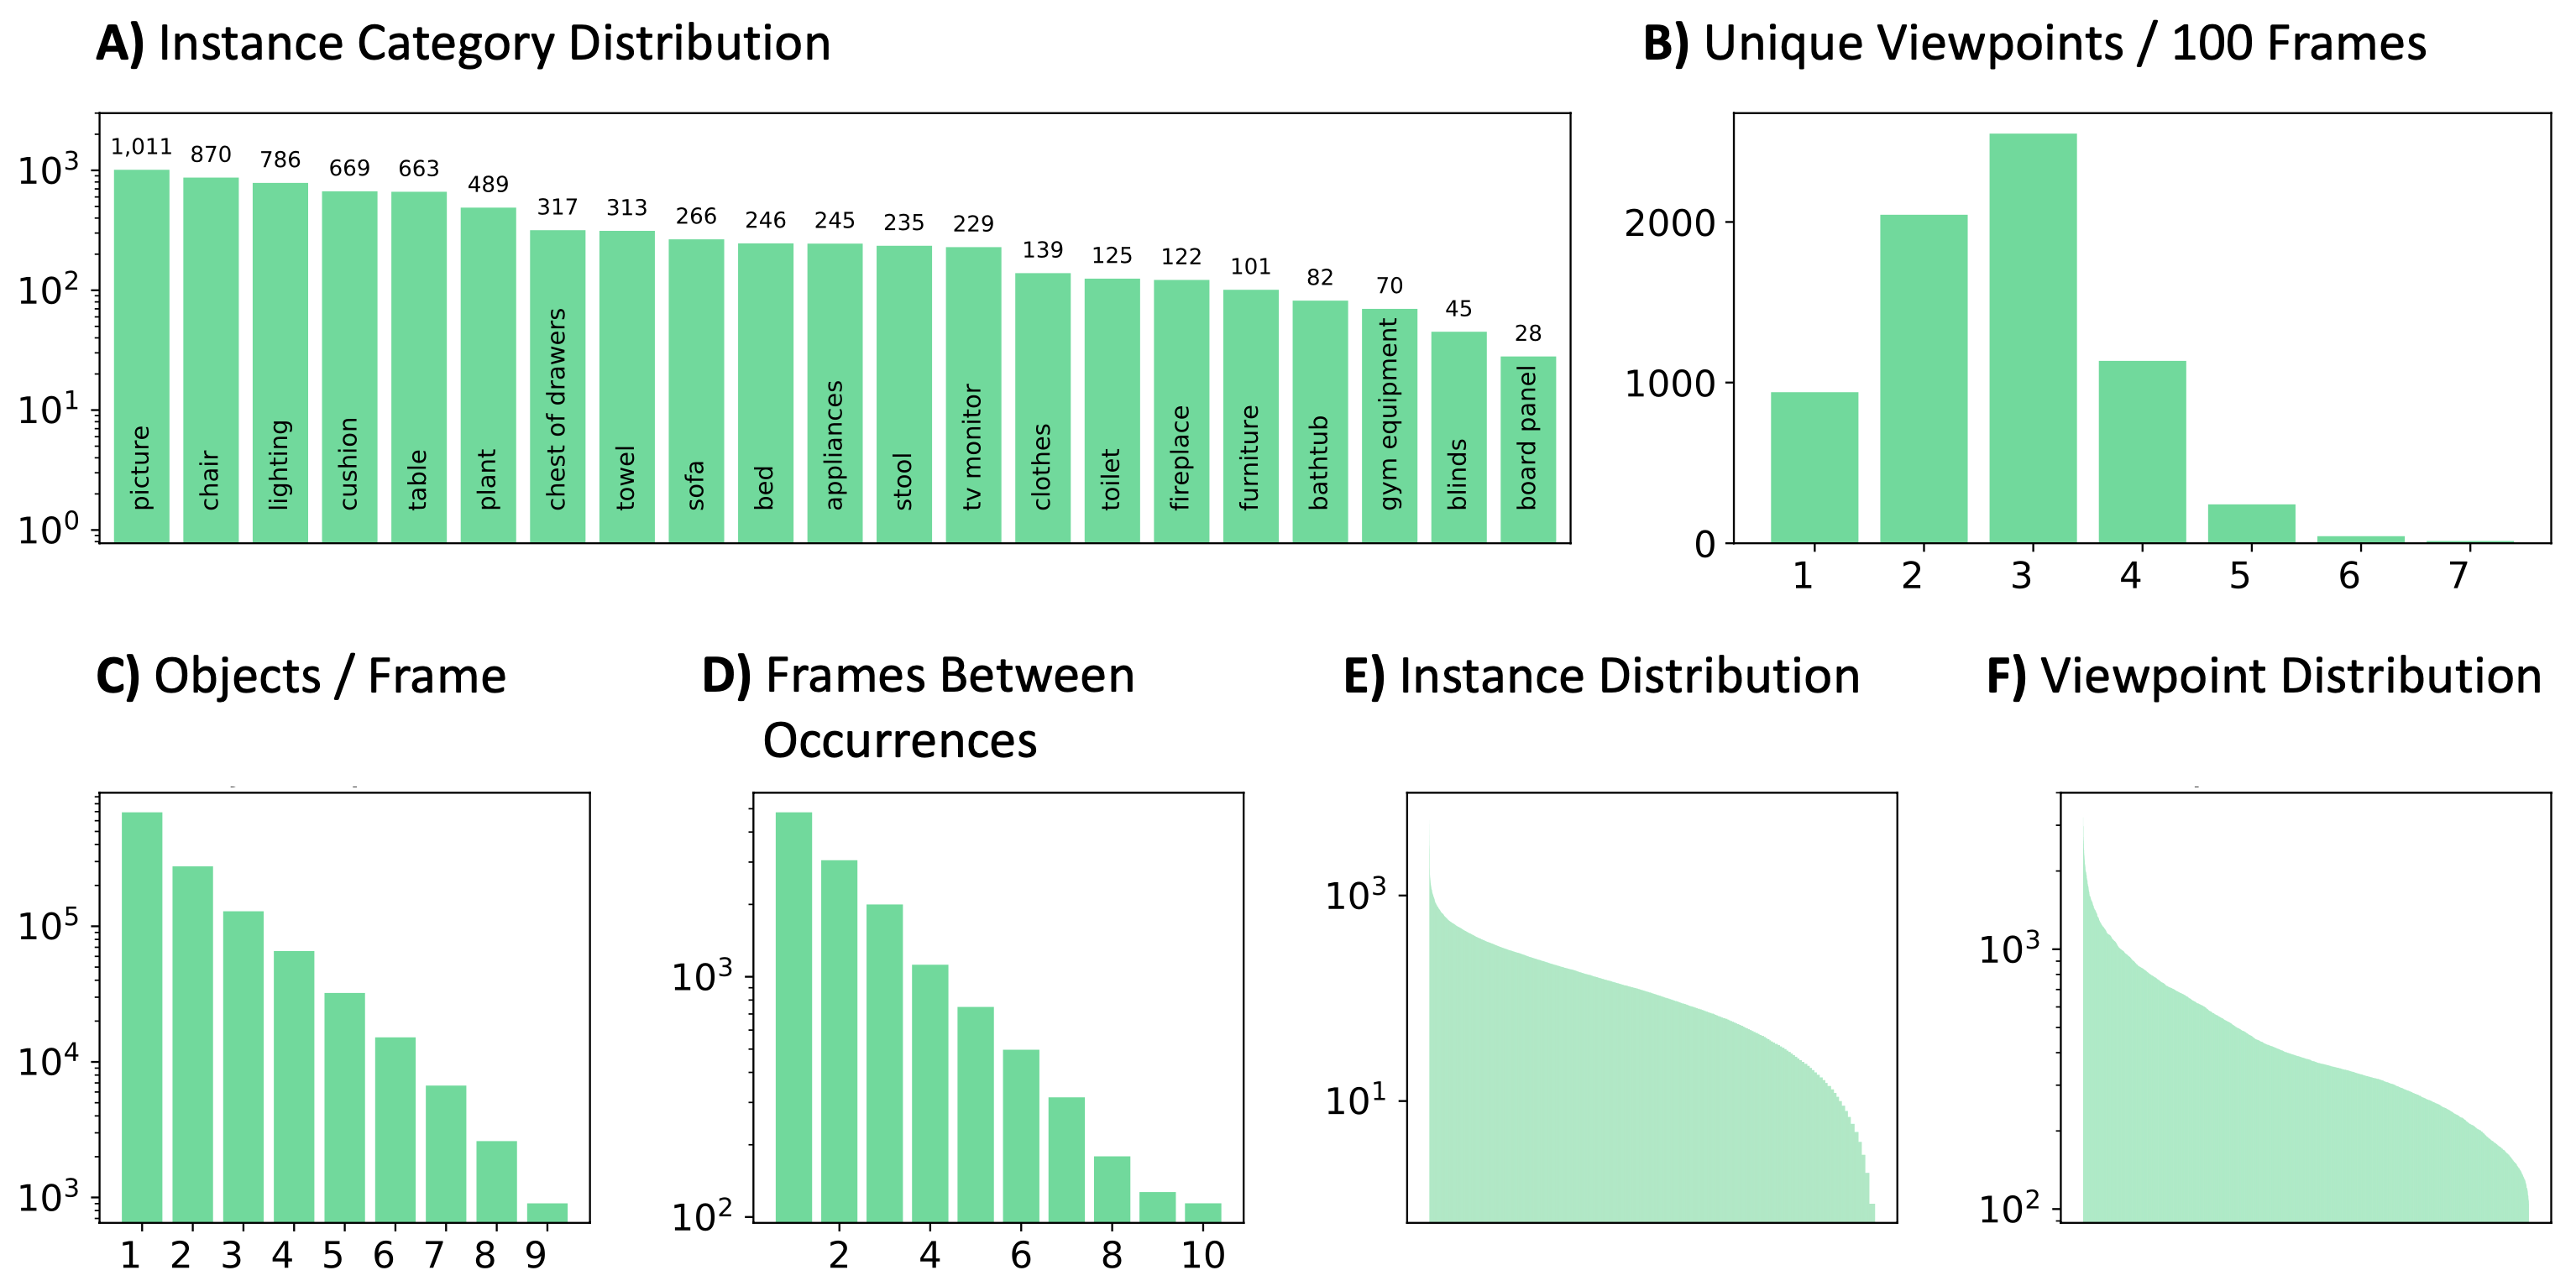
\includegraphics[width=6\textwidth]{figures/statsfull.png}
\else
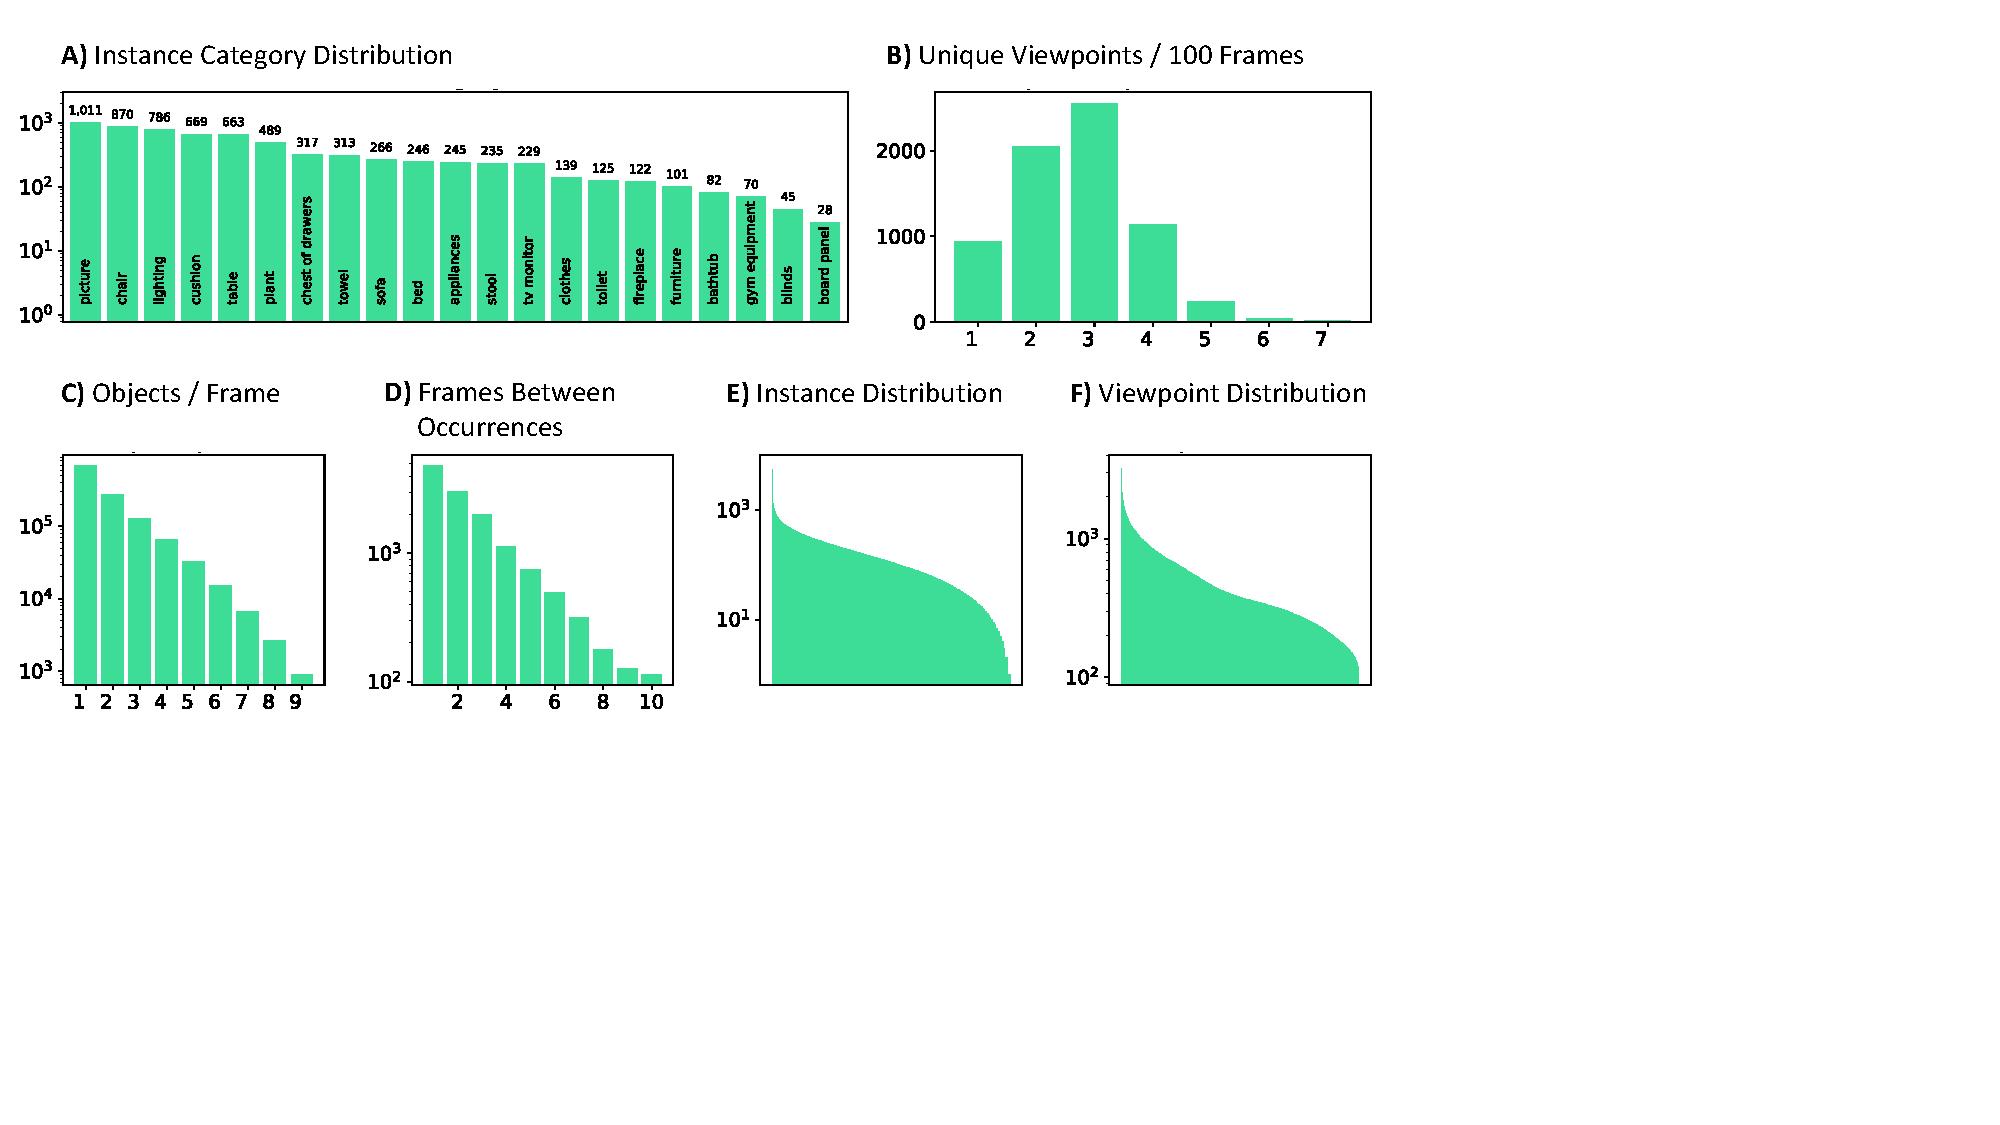
\includegraphics[width=0.9\textwidth,trim={0cm 7cm 10.2cm 0cm},clip]{figures/statsfull.pdf}
\fi
\caption{Additional statistics about our \ourroom{} dataset.}
\label{fig:additionalstats}
\end{figure}


\subsection{Training Procedure}
We use the Adam optimizer~\citep{adam} for all of our experiments, with a gradient cap of 5.0. For
\ourchar{} we train the network for 40k steps with a batch size 32 and maximum sequence length 150
across 2 GPUs and an initial learning rate 2e-3 decayed by 0.1$\times$ at 20k and 30k steps. For
\ourroom{} we train for 20k steps with a batch size 8 and maximum sequence length 100 across 4 GPUs
and an initial learning rate 1e-3 decayed by 0.1$\times$ at 8k and 16k steps. We use the BCE coefficient
$\lambda=1$  for all experiments. In semi-supervised experiments, around 30\% examples are labeled when the number of examples grows large ($\alpha = 0.3$, see Equation~\ref{eq:semisup}). Early stopping is used in \ourroom{} experiments
where the checkpoint with the highest validation AP score is chosen.
For \ourroom{}, we sample Bernoulli sequences on unlabeled inputs to 
gradually allow semi-supervised writing to the prototype memory and we find it helps training stability. The probability starts with 0.0 and increase by 0.2 every 2000 training steps until reaching 1.0.

\subsection{Data Augmentation}
For \ourchar{}, we pad the 28$\times$28 image to 32$\times$32 and then apply random cropping.

For \ourroom{}, we apply random cropping in the time dimension to get a chunk of 100 frames per
input example. We also apply random dropping of 5\% of the frames. We pad the 120$\times$160 images
to 126 $\times$ 168 and apply random cropping in each image frame. We also randomly flip the order
of the sequence (going forward or backward).


\subsection{Spatiotemporal context experiment details}
We use the Kylberg texture dataset~\citep{uppsala} without rotations. Texture classes are split into train, val, and test, defined in Table~\ref{tab:uppsalasplit}. We resize all images first to 256$\times$256. For each Omniglot image, a 28$\times$28 patch is randomly cropped from a texture image to serve as background. Random Gaussian noises with mean zero and standard deviation 0.1 are added to the background images.

For spatial background experiments, we added an additional learnable network of the same size as the main network to take the background image as input, and output the same sized embedding vector. This embedding vector is further concatenated with the main embedding vector to form the final embedding of the input. We also found that using spatially overlayed images with a single CNN can achieve similar performance as well. The final numbers are reported using the concatenation approach since it is less prone to overlay noises and is more similar to the implementation we use in the RoamingRooms experiments.

% !TEX root = ../supp.tex
\iflatexml
    \begin{table}[t]
    \begin{tabular}{clllll}
    \toprule

    \mr{3}{Train} &
    \texttt{blanket2} &
    \texttt{ceiling2} &
    \texttt{floor2} &
    \texttt{grass1} &
    \texttt{linseeds1} \\
    &
    \texttt{pearlsugar1} &
    \texttt{rice2} &
    \texttt{scarf2} &
    \texttt{screen1} &
    \texttt{seat2} \\
    &
    \texttt{sesameseeds1} &
    \texttt{stone1} & 
    \texttt{stoneslab1} & &
    \\
    \midrule

    \mr{2}{Val} &
    \texttt{blanket1} &
    \texttt{canvas1} &
    \texttt{ceiling1} & 
    \texttt{floor1} &
    \texttt{scarf1} \\
    &
    \texttt{rice1} &
    \texttt{stone2} & & & \\
    \midrule
    \mr{2}{Test} & 
    \texttt{wall1} &
    \texttt{lentils1} & 
    \texttt{cushion1} &
    \texttt{rug1} &
    \texttt{sand1} \\
    &
    \texttt{oatmeal1} &
    \texttt{stone3} &
    \texttt{seat1} & & \\
    \bottomrule
    \end{tabular}
    \caption{\textbf{Split information for the Kylberg texture dataset}. Each column is an texture type. Rows are continuation of lines.}
    \label{tab:uppsalasplit}
    \end{table}
\else
    \begin{table}[t]
    \vspace{-0.5in}
    \caption{\textbf{Split information for the Kylberg texture dataset}. Each column is an texture type. Rows are continuation of lines.}
    \label{tab:uppsalasplit}
    \begin{center}
    \begin{small}
    \begin{tabular}{clllll}
    \toprule

    \mr{3}{Train} &
    \texttt{blanket2} &
    \texttt{ceiling2} &
    \texttt{floor2} &
    \texttt{grass1} &
    \texttt{linseeds1} \\
    &
    \texttt{pearlsugar1} &
    \texttt{rice2} &
    \texttt{scarf2} &
    \texttt{screen1} &
    \texttt{seat2} \\
    &
    \texttt{sesameseeds1} &
    \texttt{stone1} & 
    \texttt{stoneslab1} & &
    \\
    \midrule

    \mr{2}{Val} &
    \texttt{blanket1} &
    \texttt{canvas1} &
    \texttt{ceiling1} & 
    \texttt{floor1} &
    \texttt{scarf1} \\
    &
    \texttt{rice1} &
    \texttt{stone2} & & & \\
    \midrule
    \mr{2}{Test} & 
    \texttt{wall1} &
    \texttt{lentils1} & 
    \texttt{cushion1} &
    \texttt{rug1} &
    \texttt{sand1} \\
    &
    \texttt{oatmeal1} &
    \texttt{stone3} &
    \texttt{seat1} & & \\
    \bottomrule
    \end{tabular}
    \end{small}
    \end{center}
    \end{table}
 \fi


\subsection{Baseline implementation details}
\paragraph{Online meta-learning (OML):} The OML  model performs one gradient descent step for each
input. In order for the model to predict unknown, we use the probability output from the softmax
layer summing across the unused units. For example, if the softmax layer has 40 units and we have
only seen 5 classes so far, then we sum the probability from the 6th to the last units. This summed
probability is separately trained with a binary cross entropy, same as in Equation~\ref{eq:loss}.

The inner learning rate is set to 1e-2 and we truncate the number of unrolled gradient descent steps
to 5/20 (\ourchar{}/\ourroom{}), in order to make the computation feasible. For \ourchar{}, the
network is trained with a batch size 32 across 2 GPUs, for a total of 20k steps, with an initial
learning rate 2e-3 decayed by 0.1 at 10k and 16.7k steps. For \ourroom{}, the network is trained
with a batch size 8 across 4 GPUs, for a total of 16k steps, with an initial learning rate 1e-3
decayed by 0.1 at 6.4k and 12.8k steps.

\paragraph{Long short-term memory (LSTM):} We apply a stacked two layer LSTM with 256 hidden
dimensions. Inputs are $\bh_t^{\text{CNN}}$ concatenated with the label one-hot vector. If an
example is unlabeled, then the label vector is all-zero. We directly apply a linear layer on top of
the LSTM to map the LSTM memory output into classification logits, and the last logit is the binary
classification logit reserved for unknown. The training procedure is the same as our CPM model.

\paragraph{Differentiable neural computer (DNC):} In order to make the DNC model work properly, we
found that it is sometimes helpful to pretrain the CNN weights. Simply initializing from scratch and
train CNN+DNC end-to-end sometimes results in poor performance. We hypothesize that the attention
structure in the DNC model is detrimental to representation learning. Therefore, for \ourchar{}
experiments, we use pretrained ProtoNet weights for solving 1-shot 5-way episodes to initialize the
CNN, and we keep finetuning the CNN weights with 10\% of the full learning rate. For \ourroom{}
experiments, we train the full model end-to-end from scratch.

The DNC is also modified so that it is more effective using the label information from the input. In
the original MANN paper~\citep{mann} for one-shot learning, the input features $\bh_t^{\text{CNN}}$
and the label one-hot ID are simply concatenated to feed into the LSTM controller of MANN. We find
that it is beneficial to directly add label one-hot vector as an input to the write head that
generates the write attention and the write content.  Similar to the LSTM model, the memory readout is also sent to a
linear layer in order to get the final classification logits, and the last logit is the binary
classification logit reserved for the unknowns. Finally we remove the linkage prediction part of the DNC
due to training instability.

The controller LSTM has 256 hidden dimensions, and the memory has 64 slots each with 64 dimensions.
There are 4 read heads and 4 write heads. The training procedure is the same as CPM.

\paragraph{Online ProtoNet:} Online ProtoNet is our modification of the original
ProtoNet~\citep{protonet}. It is similar to our CPM model without the contextual RNN. The feature
from the CNN is directly written to the prototype memory. In addition, we do not predict the control
hyperparameters $\beta^{\{r,w\}}_t,\gamma^{\{r,w\}}_t$ from the RNN and they are learned as regular parameters. The training procedure is the same as CPM.

\paragraph{Online MatchingNet:} Online MatchingNet is our modification of the original
MatchingNet~\citep{matchingnet}. We do not consider the context embedding in the MatchingNet paper
since it was originally designed for the entire episode using an attentional RNN encoder. It is
similar to online ProtoNet but instead of doing online averaging, it directly stores each example
and its class. Since it is an example-based storage, we did not extend it to learn from
unlabeled examples, and all unlabeled examples are skipped. We use a similar decision rule to
determine whether an example belongs to a known cluster by looking at the distance to the nearest
exemplar stored in the memory, shifted by $\beta$ and scaled by $1/\gamma$. Note that online
MatchingNet is not efficient at memory storage since it scales with the number of steps in the
sequence. In addition, we use the negative Euclidean distance as the similarity function. The training
procedure is the same as CPM.

\paragraph{Online infinite mixture prototypes (IMP):} Online IMP is proposed as a mix of prototype and example-based storage by allowing a class to have multiple clusters. If an
example is classified as unknown or it is unlabeled, we will assign its cluster based on our
prediction, which either assigns it to one of the existing clusters or creates a new cluster,
depending on its distance to the nearest cluster. If a cluster with an unknown label later is
assigned with an example with a known class, then the cluster label will also be updated. We use the same
decision rule as online ProtoNet to determine whether an example belongs to a known cluster by
looking at the distance to the nearest cluster, shifted by $\beta$ and scaled by $1/\gamma$. As
described above, online IMP has the capability of learning from unlabeled examples, unlike online
MatchingNet. However similar to online MatchingNet, online IMP is also not efficient at memory
storage since in the worst case it also scales with the number of steps in the sequence. Again, the
training procedure is the same as CPM.

\section{Additional Experimental Results}
\label{sec:additionalresults}
\subsection{Effect of Forgetting}
We report the effect of forgetting of \ourroom{} and \ourimg{} in Table~\ref{tab:forgetroom} and \ref{tab:forgetimagenet}.
\iflatexml
\begin{table}[t]
    \centering
    \begin{tabular}{ccccccc|cccccc}
    \toprule
    & \mc{6}{c|}{\textbf{Supervised}} & \mc{6}{c}{\textbf{Semi-Supervised}}\\
                &   1 - 2&      3 - 5&      6 - 10&     11 - 20&    21 - 50&    51 - 100&
                    1 - 2&      3 - 5&      6 - 10&     11 - 20&    21 - 50&    51 - 100\\
    OPN 1-Shot  &   93.5&   	89.3&	    79.4&	    67.2&	    60.3&	    60.1&
                    86.5&	    83.6&	    76.3&	    68.4&	    64.7&	    61.5\\
    CPM 1-Shot  &   \bf{95.7}&	\bf{92.2}&  \bf{85.7}&	\bf{75.2}&	\bf{70.0}&  \bf{66.4}&
                    \bf{91.0}&	\bf{88.7}&	\bf{82.9}&	\bf{77.0}&  \bf{72.2}&	\bf{66.5}\\
    OPN 3-Shot  &   95.1&	    91.8&	    85.6&   	78.2&	    74.6&	    73.8&
                    92.6&       88.0&	    85.1&	    81.1&	    80.6&	    76.7\\
    CPM 3-Shot  &   \bf{96.1}&	\bf{93.8}&	\bf{87.7}&	\bf{81.4}&  \bf{79.1}&	\bf{78.2}&
                    \bf{94.8}&  \bf{91.0}&	\bf{86.9}&	\bf{83.1}&	\bf{82.7}&  \bf{79.2}\\
    \bottomrule
    \end{tabular}
    \caption{\textbf{Effect of forgetting over a time interval on \ourroom{}.} Average accuracy vs. the number of time steps since the model has last seen the label of a particular class.}
    \label{tab:forgetroom}
\end{table}

\begin{table}[t]
    \centering
    \begin{tabular}{ccccccc|cccccc}
    \toprule
    & \mc{6}{c|}{\bf Supervised} & \mc{6}{c}{\bf Semi-Supervised}\\
                &   1 - 2&      3 - 5&      6 - 10&     11 - 20&    21 - 50&    51 - 100&
                    1 - 2&      3 - 5&      6 - 10&     11 - 20&    21 - 50&    51 - 100\\
    OPN 1-Shot  &   40.8&	35.9&	33.0&	\bf{30.7}&	\bf{27.0}&	\bf{21.4}&
                    40.5&	37.7&	35.9&	\bf{33.7}&	\bf{31.5}&	\bf{28.4}\\
    CPM 1-Shot  &   \bf{67.5}&	\bf{52.9}&	\bf{35.5}&	24.2&	18.3&	13.8&
                    \bf{60.4}&	\bf{51.3}&	\bf{39.5}&	26.6&	21.8&	15.4\\
    OPN 3-Shot  &   52.5&	50.3&	\bf{48.8}&	\bf{47.2}&	\bf{44.4}&	\bf{42.3}&
                    57.6&	55.1&	\bf{54.6}&	\bf{52.3}&	\bf{52.1}&	\bf{49.5}\\
    CPM 3-Shot  &   \bf{77.8}&	\bf{64.5}&	46.6&	32.9&	24.7&	17.9&
                    \bf{76.1}&	\bf{61.8}&	48.6&	30.5&	24.1&	15.6\\
    \bottomrule
    \end{tabular}
    \caption{\textbf{Effect of forgetting over a time interval on \ourimg{}.} Average accuracy vs. the number of time steps since the model has last seen the label of a particular class.}
    \label{tab:forgetimagenet}
\end{table}

\else
\begin{table}[t]
\vspace{-0.5in}
    \centering
    \caption{\textbf{Effect of forgetting over a time interval on \ourroom{}.} Average accuracy vs. the number of time steps since the model has last seen the label of a particular class.}
    
    \resizebox{\textwidth}{!}{
    \begin{tabular}{ccccccc|cccccc}
    \toprule
    & \mc{6}{c}{\bf Supervised} & \mc{6}{c}{\bf Semi-Supervised}\\
                &   1 - 2&      3 - 5&      6 - 10&     11 - 20&    21 - 50&    51 - 100&
                    1 - 2&      3 - 5&      6 - 10&     11 - 20&    21 - 50&    51 - 100\\
    \midrule
    OPN 1-Shot  &   93.5&   	89.3&	    79.4&	    67.2&	    60.3&	    60.1&
                    86.5&	    83.6&	    76.3&	    68.4&	    64.7&	    61.5\\
    CPM 1-Shot  &   \bf{95.7}&	\bf{92.2}&  \bf{85.7}&	\bf{75.2}&	\bf{70.0}&  \bf{66.4}&
                    \bf{91.0}&	\bf{88.7}&	\bf{82.9}&	\bf{77.0}&  \bf{72.2}&	\bf{66.5}\\
    \midrule
    OPN 3-Shot  &   95.1&	    91.8&	    85.6&   	78.2&	    74.6&	    73.8&
                    92.6&       88.0&	    85.1&	    81.1&	    80.6&	    76.7\\
    CPM 3-Shot  &   \bf{96.1}&	\bf{93.8}&	\bf{87.7}&	\bf{81.4}&  \bf{79.1}&	\bf{78.2}&
                    \bf{94.8}&  \bf{91.0}&	\bf{86.9}&	\bf{83.1}&	\bf{82.7}&  \bf{79.2}\\
    \bottomrule
    \end{tabular}}
    \label{tab:forgetroom}
\end{table}

\begin{table}[t]
\vspace{-0.2in}
    \centering
    \caption{\textbf{Effect of forgetting over a time interval on \ourimg{}.} Average accuracy vs. the number of time steps since the model has last seen the label of a particular class.}
    
    \resizebox{\textwidth}{!}{
    \begin{tabular}{ccccccc|cccccc}
    \toprule
    & \mc{6}{c}{\bf Supervised} & \mc{6}{c}{\bf Semi-Supervised}\\
                &   1 - 2&      3 - 5&      6 - 10&     11 - 20&    21 - 50&    51 - 100&
                    1 - 2&      3 - 5&      6 - 10&     11 - 20&    21 - 50&    51 - 100\\
    \midrule
    OPN 1-Shot  &   40.8&	35.9&	33.0&	\bf{30.7}&	\bf{27.0}&	\bf{21.4}&
                    40.5&	37.7&	35.9&	\bf{33.7}&	\bf{31.5}&	\bf{28.4}\\
    CPM 1-Shot  &   \bf{67.5}&	\bf{52.9}&	\bf{35.5}&	24.2&	18.3&	13.8&
                    \bf{60.4}&	\bf{51.3}&	\bf{39.5}&	26.6&	21.8&	15.4\\
    \midrule
    OPN 3-Shot  &   52.5&	50.3&	\bf{48.8}&	\bf{47.2}&	\bf{44.4}&	\bf{42.3}&
                    57.6&	55.1&	\bf{54.6}&	\bf{52.3}&	\bf{52.1}&	\bf{49.5}\\
    CPM 3-Shot  &   \bf{77.8}&	\bf{64.5}&	46.6&	32.9&	24.7&	17.9&
                    \bf{76.1}&	\bf{61.8}&	48.6&	30.5&	24.1&	15.6\\
    \bottomrule
    \end{tabular}}
    \label{tab:forgetimagenet}
\end{table}


% \subsection{Video Visualization}
% We include video visualization of \ourroom{} sequences here:
% \footnote{\url{https://drive.google.com/drive/folders/1gBJBFdNb0EOvK6CEYKxIL1Og0_jrqrbK}}. Our CPM
% model prediction can be found here:
% \footnote{\url{https://drive.google.com/drive/folders/1rp9xxAccrZyffngFdtoS9Bl6P9uxJ9xN}}.

\subsection{Embedding Visualization} 
Figure~\ref{fig:tsne} shows the learned embedding of each example in Online ProtoNet vs. our CPM
model in \ourchar{} sequences, where colors indicate environment IDs. In Online ProtoNet, the
example features does not reflect the temporal context, and as a result, colors are scattered across
the space. By contrast, in the CPM embedding visualization, colors are clustered together and we see
a smoother transition of environments in the embedding space.

% !TEX root = ../supp.tex
\begin{figure}[t]
\centering
% \vspace{-0.2in}
\iflatexml
    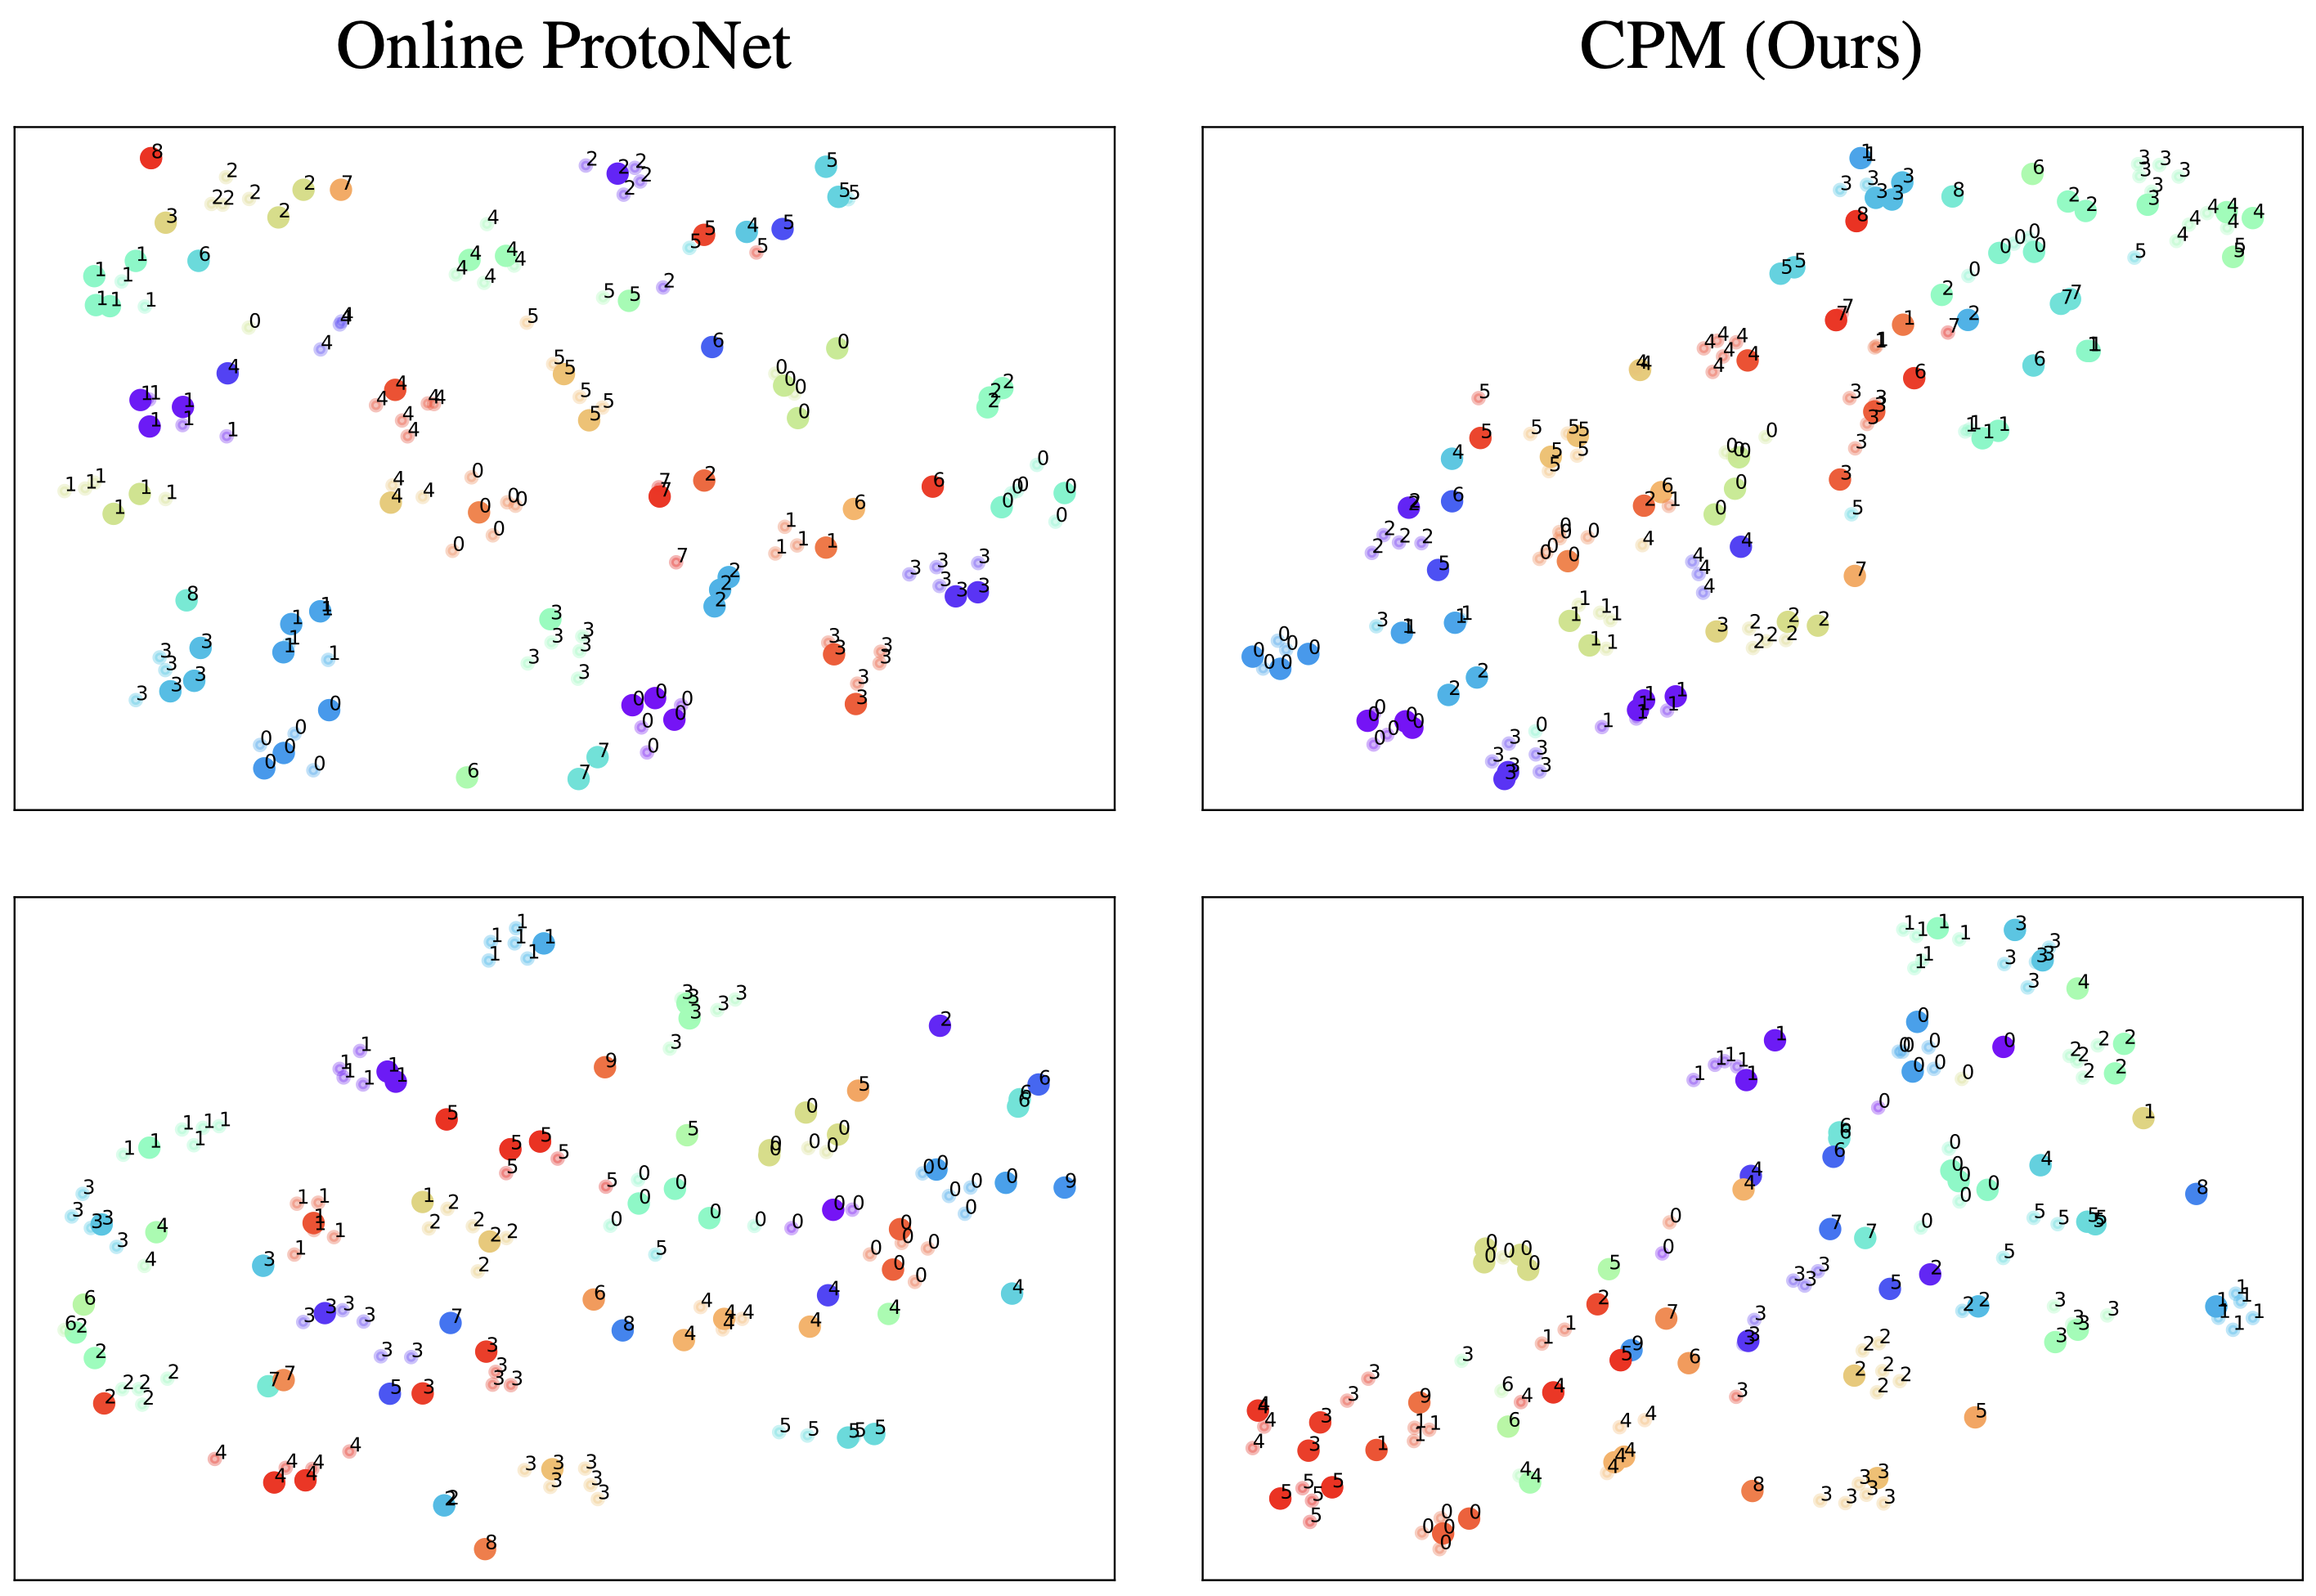
\includegraphics[width=6\linewidth]{figures/omniglot-tsne.png}
\else
    \begin{tabular}{cc}
    Online ProtoNet & CPM (Ours) \\
    \includegraphics[height=3.8cm, trim={2.5cm 1cm 2cm 1cm}, clip]{figures/omniglot-protonet-tsne/tsne-003.pdf}
    &
    \includegraphics[height=3.8cm, trim={2.5cm 1cm 2cm 1cm}, clip]{figures/omniglot-cpm-tsne/tsne-003.pdf}
    \\
    \includegraphics[height=3.8cm, trim={2.5cm 1cm 2cm 1cm}, clip]{figures/omniglot-protonet-tsne/tsne-008.pdf}
    &
    \includegraphics[height=3.8cm, trim={2.5cm 1cm 2cm 1cm}, clip]{figures/omniglot-cpm-tsne/tsne-008.pdf}
    \end{tabular}
\fi
\caption{\textbf{Embedding space visualization of \ourchar{} sequences using t-SNE~\citep{tsne}}. Different color
denotes different environments. Text labels (relative to each environment) are annotated beside the
scatter points. Unlabeled examples shown in smaller circles with lighter colors. \textbf{Left:}
Online ProtoNet; \textbf{Right:} CPM. The embeddings learned CPM model shows a smoother transition
of classes based on their temporal environments.}
\label{fig:tsne}
\end{figure}


\subsection{Control Parameters vs. Time}
Finally we visualize the control parameter values predicted by the RNN in
Figure~\ref{fig:betagamma}. We verify that we indeed need two sets of $\beta$ and $\gamma$ for read
and write operations separately as they learn different values. $\beta^w$ is smaller than $\beta^r$
which means that the network is more conservative when writing to prototypes. $\gamma^w$ grows
larger over time, which means that the network prefers a softer slope when writing to prototypes
since in the later stage the prototype memory has already stored enough content and it can grow
faster, whereas in the earlier stage, the prototype memory is more conservative to avoid embedding
vectors to be assigned to wrong clusters.

% !TEX root = ../supp.tex
\begin{figure}
\centering
% \vspace{-0.1in}
\iflatexml
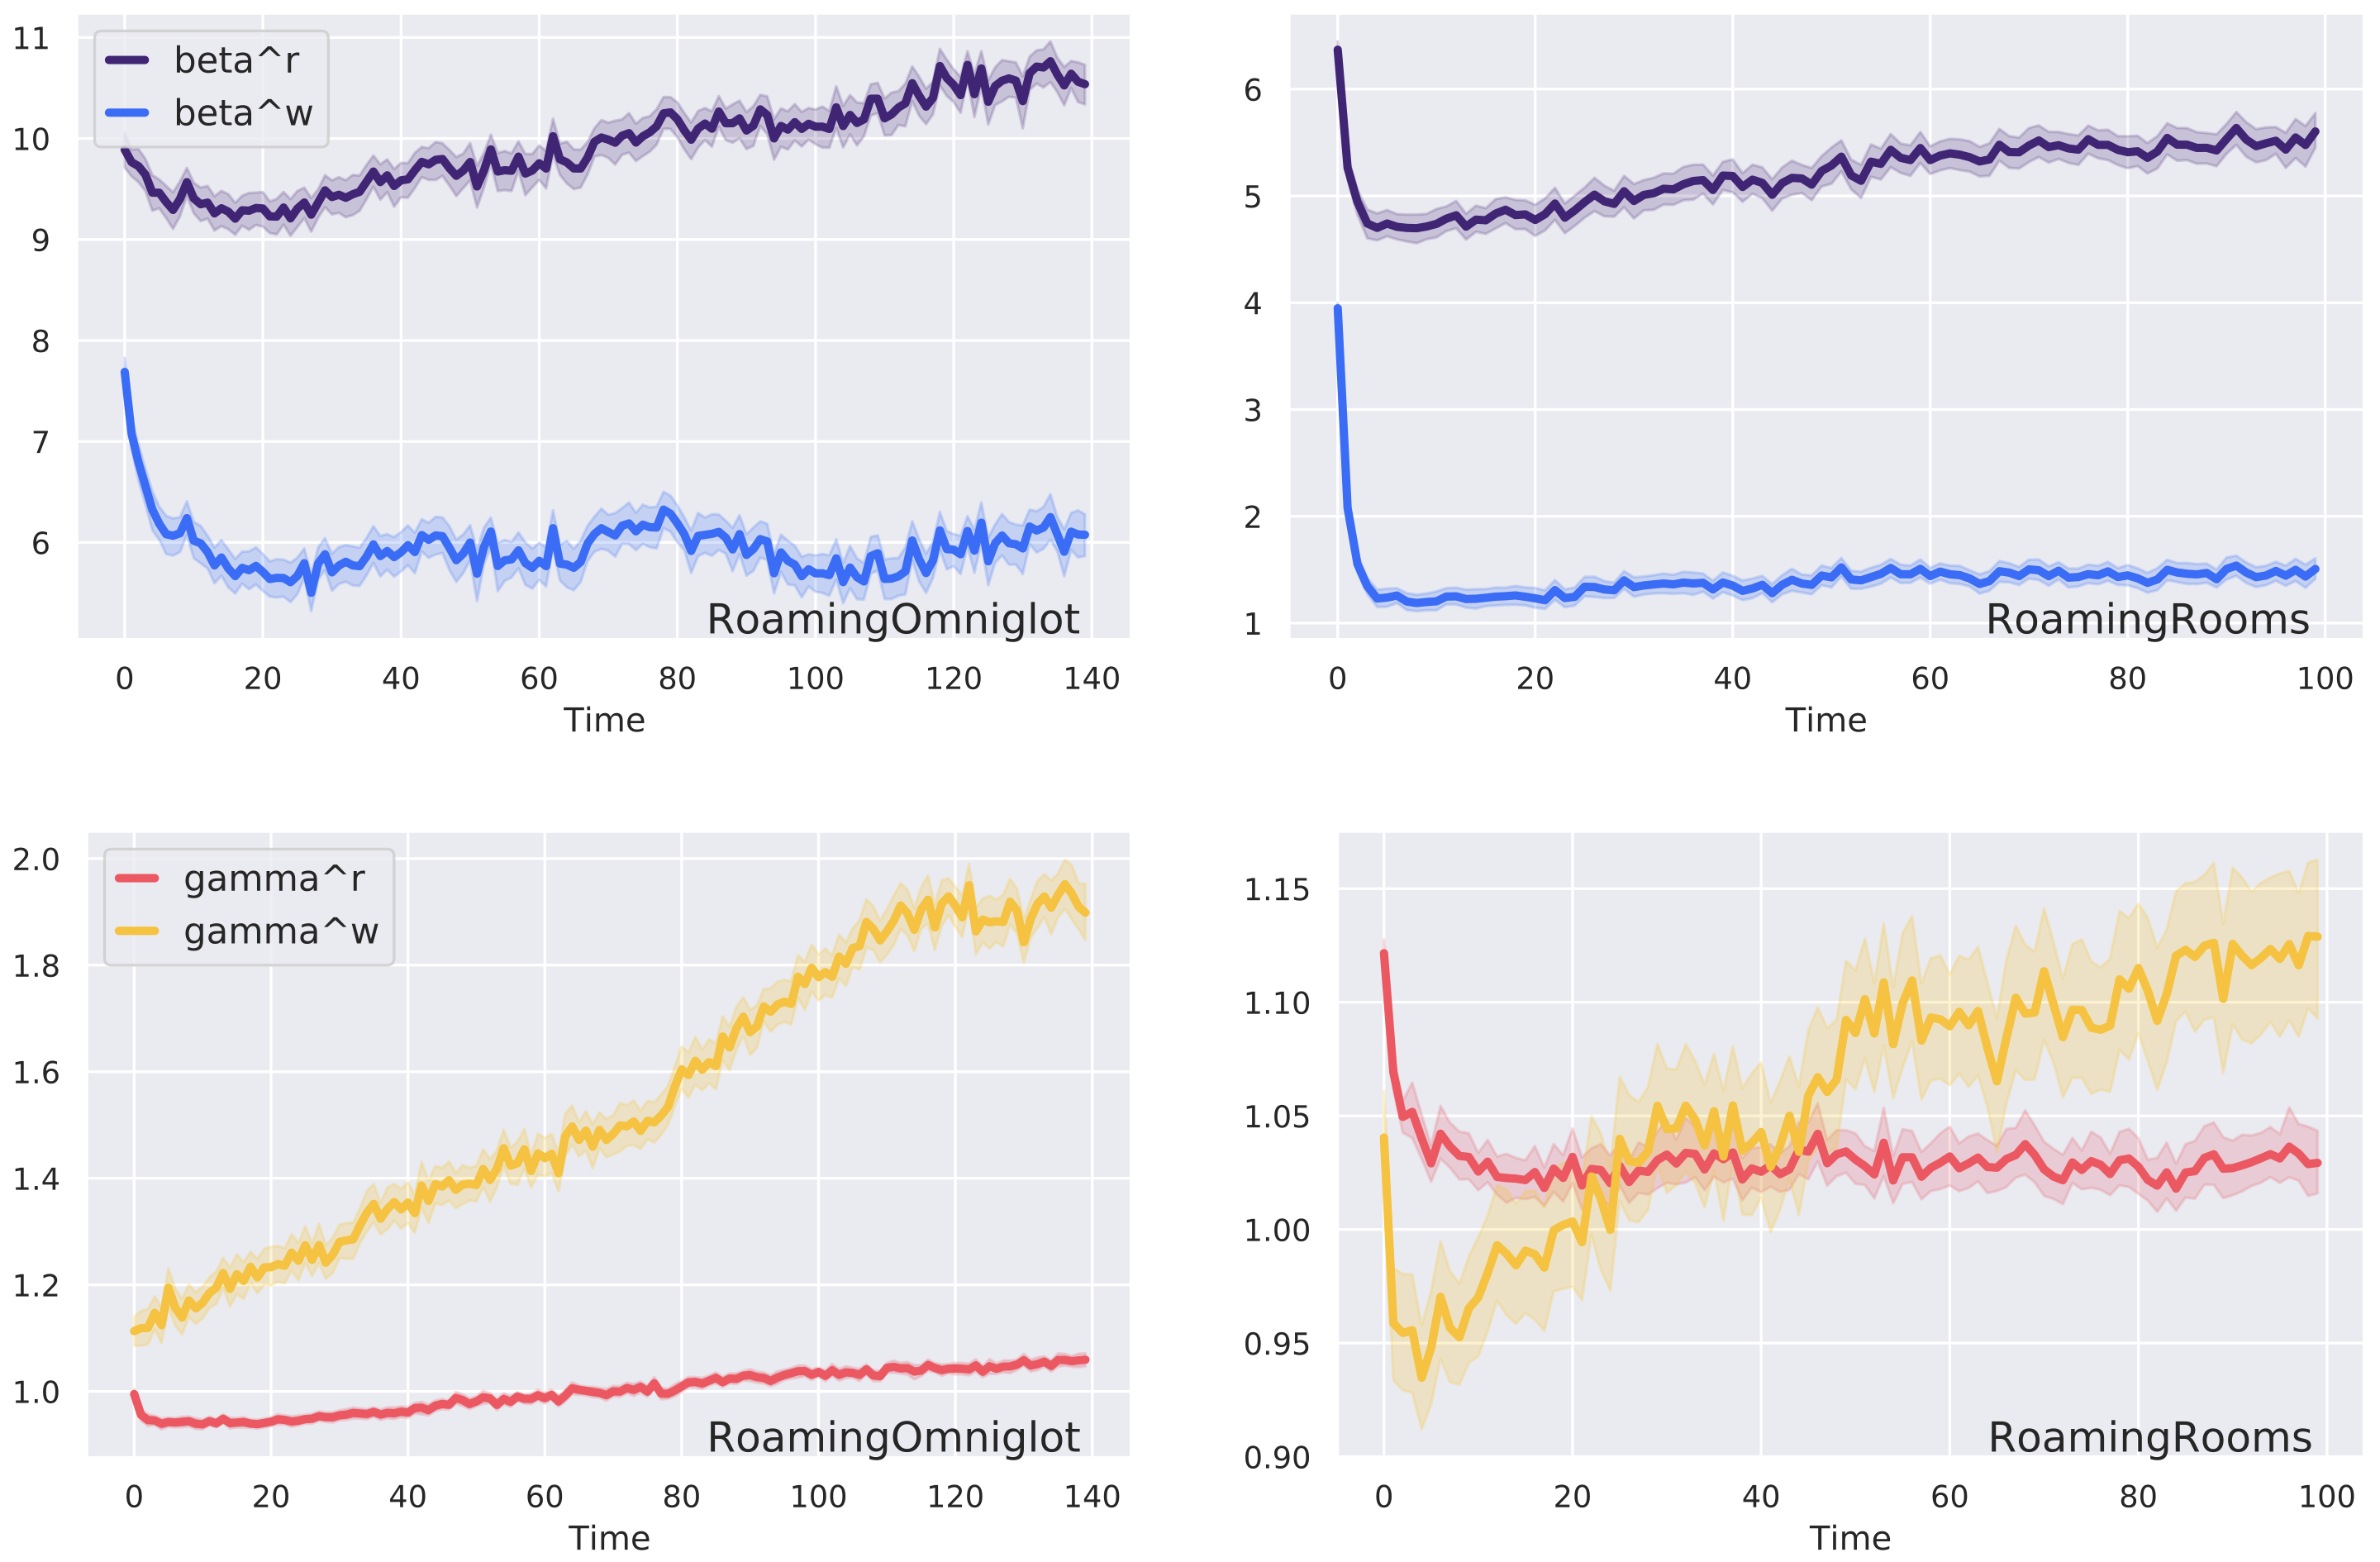
\includegraphics[width=6\linewidth]{figures/beta-gamma.png}
\else
\begin{tabular}{cc}
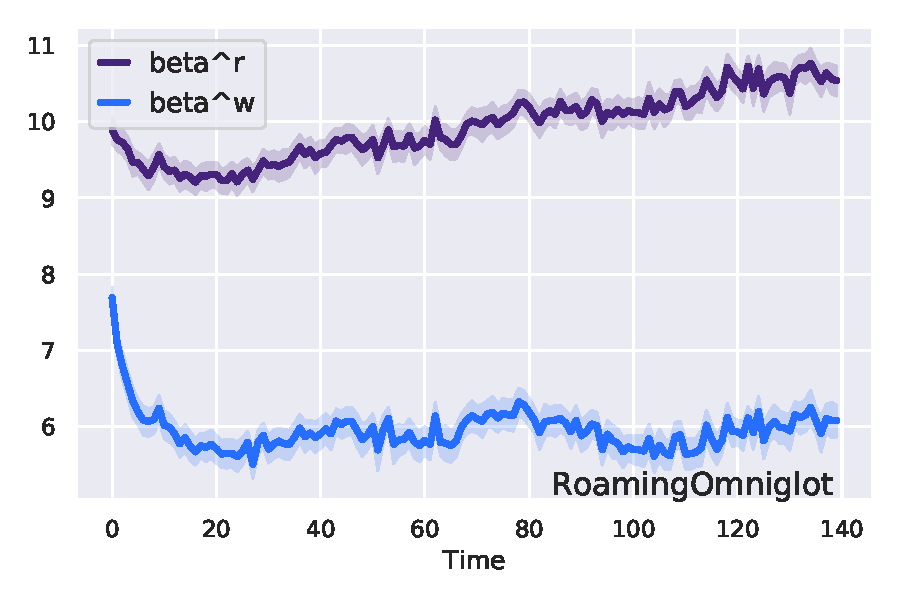
\includegraphics[height=4.0cm,trim={0.3cm 0cm 0.5cm 0},clip]{figures/omniglot-beta.pdf}
\quad
&
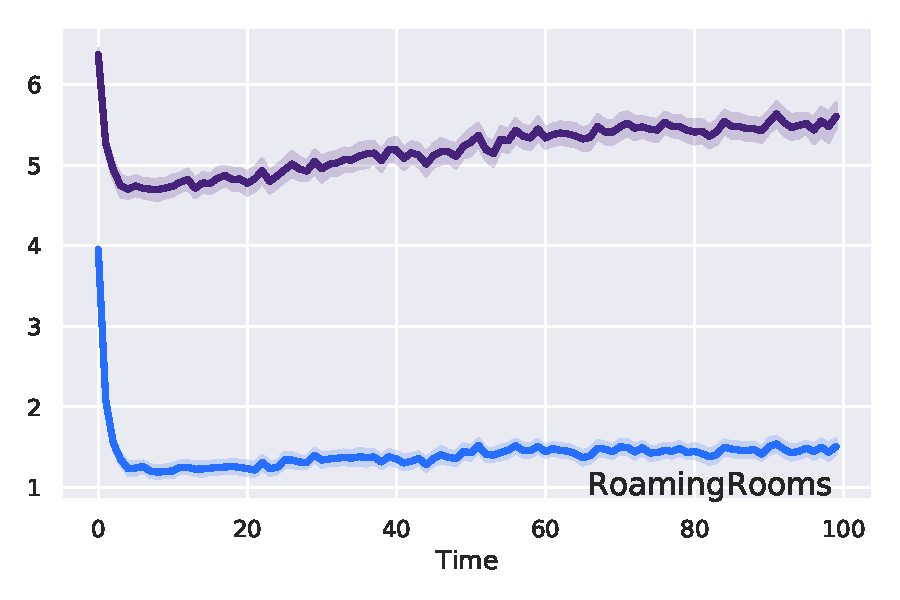
\includegraphics[height=4.0cm,trim={0.3cm 0cm 0cm 0},clip]{figures/matterport-beta.pdf}
\\
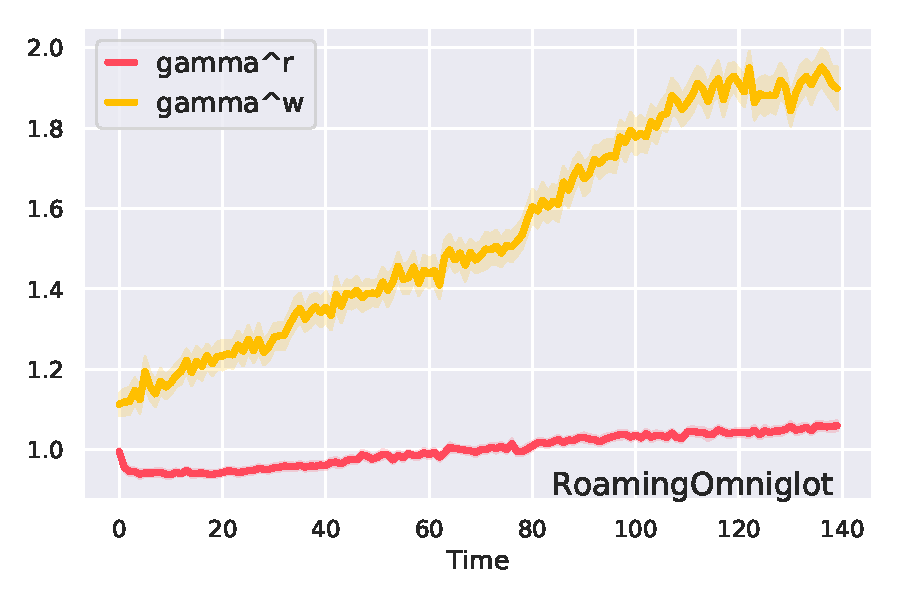
\includegraphics[height=4.0cm,trim={0.3cm 0cm 0.5cm 0},clip]{figures/omniglot-gamma.pdf}
\quad
&
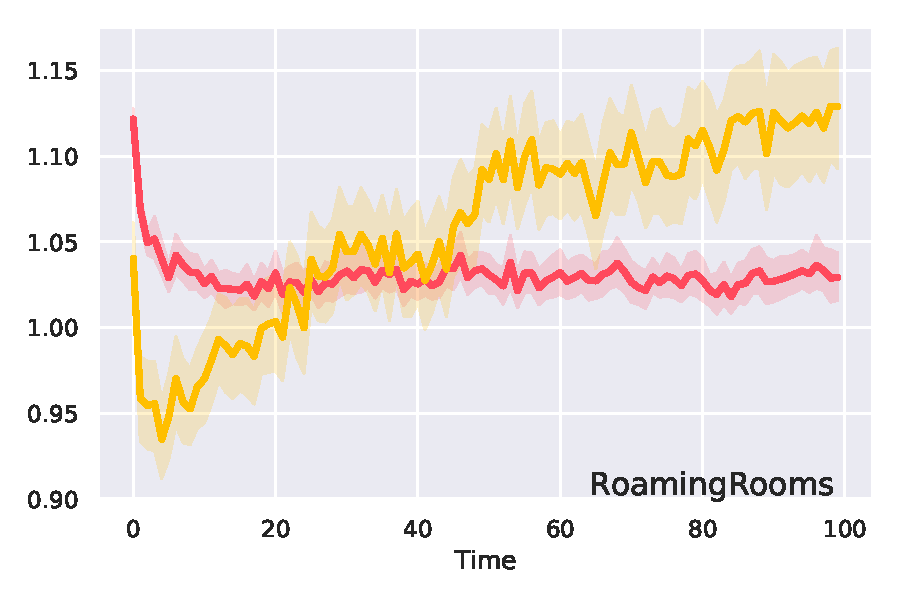
\includegraphics[height=4.0cm,trim={0.3cm 0cm 0cm 0},clip]{figures/matterport-gamma.pdf}
\\
\end{tabular}
\vspace{-0.1in}
\fi
\caption{\textbf{CPM control parameters ($\beta^{r,w}, \gamma^{r,w}$) vs. time.}
\textbf{Left:} \ourchar{} sequences; \textbf{Right:} \ourroom{} sequences; \textbf{Top:}
$\beta^{r,w}$ the threshold parameter; \textbf{Bottom:} $\gamma^{r,w}$ the temperature parameter.}
\label{fig:betagamma}
\end{figure}


\fi

\end{document}
